\documentclass[11pt,a4paper,twoside,slovene]{book}
% Za latex matrike: http://en.wikibooks.org/wiki/LaTeX/Mathematics
%%% Uvoženi paketi in uporaba pravil.
\usepackage[slovene]{babel}
\usepackage[utf8]{inputenc}
\usepackage{graphicx}
\usepackage{subfigure}
\usepackage{url}
\usepackage{fancyhdr}
\usepackage{amsmath,amssymb,amsfonts}
\usepackage{mathtools}
\usepackage{theorem}
\usepackage[unicode]{hyperref}
\usepackage{calrsfs}
\usepackage{gensymb}
\usepackage{tikz}
\overfullrule=15pt % oznaci predolgo vrstico
\DeclareMathAlphabet{\pazocal}{OMS}{zplm}{m}{n}

%%% Makroji
\newcommand{\set}[1]{\left\{#1\right\}}
\newcommand{\R}{\mathbb R}
\newcommand{\N}{\mathbb N}
\newcommand{\Z}{\mathbb Z}
\renewcommand{\C}{\mathbb C}
\newcommand{\Q}{\mathbb Q}
\newcommand{\NN}{\pazocal{N}}
\newcommand{\F}{\pazocal{F}}
\renewcommand{\O}{\pazocal{O}}
\renewcommand{\l}{\ell}
\renewcommand{\L}{\mathfrak L}
\newcommand{\CC}{\pazocal C}
\newcommand{\LL}{\pazocal{L}}
\newcommand{\I}{\pazocal{I}}
\newcommand{\J}{\pazocal{J}}
\newcommand{\fun}[3]{#1 : #2 \to #3}
\newcommand{\norm}[1]{\left\|#1\right\|}
\newcommand{\abs}[1]{\left|#1\right|}
\newcommand{\argmax}{\textup{argmax}}
\newcommand{\argmin}{\textup{argmin}}
\newcommand{\getvalue}[2]{#1 \gets #2}
\newcommand{\iu}{{i\mkern1mu}}
\renewcommand{\i}{\imath}

%%% Definicije okolij za izreke ipd.
{
   \theorembodyfont{\itshape}
   \newtheorem{trditev}{Trditev}[section]
   \newtheorem{izrek}[trditev]{Izrek}
   \newtheorem{lema}[trditev]{Lema}
   \newtheorem{izjava}[trditev]{Izjava}
   \newtheorem{posledica}[trditev]{Posledica}
   \newtheorem{hipoteza}[trditev]{Hipoteza}
 }

 {
   \theorembodyfont{\rmfamily}
   \newtheorem{definicija}[trditev]{Definicija}
   \newtheorem{primer}[trditev]{Primer}
   \newtheorem{opomba}[trditev]{Opomba}
 }

%%% Okolje za dokaze.
\newenvironment{dokaz}{
  \goodbreak\par
  \textit{Dokaz.}%
}{%
  \nopagebreak
  \hfill{\vrule width 1ex height 1ex depth 0ex}
  \medskip
  \goodbreak
}

%%% Okolje za algoritme
\usepackage{algpseudocode, algorithm}
\floatname{algorithm}{Algoritem}
\renewcommand{\algorithmicrequire}{\textbf{Vhodni podatki:}}
\renewcommand{\algorithmicensure}{\textbf{Izhodni podatki:}}

%%% Stil strani & margine

%% A4 stran = 210mm x 297mm
%% sirino besedila nastavimo na 170mm, visino na 247mm

\setlength{\textwidth}{15cm}
\setlength{\textheight}{224mm}

\setlength{\topmargin}{0cm}
\setlength{\evensidemargin}{0cm}
\setlength{\oddsidemargin}{\paperwidth}
\addtolength{\oddsidemargin}{-\textwidth}
\addtolength{\oddsidemargin}{-2in}

%TODO Ne dela pri meni ... čemu je to namenjeno???
%\addtolength{\headwidth}{\marginparsep}
%\addtolength{\headwidth}{\marginparwidth}

\pagestyle{fancyplain}

\renewcommand{\headrulewidth}{0.2pt}
\addtolength{\headheight}{2pt}

\renewcommand{\chaptermark}[1]{\markboth{#1}{}}
\renewcommand{\sectionmark}[1]{\markright{\thesection\ #1}}

\lhead[\fancyplain{}{{\thepage}}]%
      {\fancyplain{}{{\rightmark}}}
\rhead[\fancyplain{}{{\leftmark}}]%
      {\fancyplain{}{\thepage}}
\cfoot{}
\lfoot[]{}
\rfoot[]{}

%% Define a new 'leo' style for the package that will use a smaller font.
\makeatletter
\def\url@leostyle{%
  \@ifundefined{selectfont}{\def\UrlFont{\sf}}{%
    \def\UrlFont{\small\sffamily}}\Url@do
}
\makeatother

%% Now actually use the newly defined style.
\urlstyle{leostyle}
\newcommand{\myurl}[1]{\url{#1}}

%--------------------------------------------------------------------
%--------------------------------------------------------------------

\author{Katarina Zadražnik}
\title{Likovno upodabljanje slik}

%--------------------------------------------------------------------
%--------------------------------------------------------------------

\begin{document}
\frontmatter
\pagestyle{empty}

%--------------------------------------------------------------------
%--------------------------------------------------------------------
% NASLOVNA STRAN
\begin{flushleft}
\noindent
\textsc{\Large UNIVERZA V LJUBLJANI}\\
\textsc{\Large FAKULTETA ZA MATEMATIKO IN FIZIKO}\\
\medskip
\Large Matematika -- 2.\ stopnja
\end{flushleft}

\vfill

\begin{center}
 {\LARGE Katarina Zadražnik}

  \bigskip
  \medskip
  {\bfseries {\Huge Likovno upodabljanje slik}}

  \bigskip
  \medskip

  {\LARGE Magistrsko delo}
  
  \bigskip
  \medskip
  
  {\Large Mentor: prof.\ dr.\ Andrej Bauer}
\end{center}

\vfill
\vfill
\noindent
{\Large Ljubljana, 2016}

\cleardoublepage

%--------------------------------------------------------------------
%--------------------------------------------------------------------
% IZJAVA
\null
\vfill
\noindent Podpisana {Katarina Zadražnik} izjavljam: % FIXME Avtor
\begin{itemize}
 \item[--] da sem magistrsko delo z naslovom Likovno upodabljanje slik izdelala samostojno pod mentorstvom {prof.\ dr.\ Andreja Bauerja}, ter % FIXME Naslov, mentor in somentor, če je
 \item[--] da Fakulteti za matematiko in fiziko Univerze v Ljubljani dovoljujem objavo elektronske oblike svojega dela na spletnih straneh.
\end{itemize}
Ljubljana, \today \hfill Podpis:\hspace{5cm} % Datum se nastavi na ``danes''

\cleardoublepage

%--------------------------------------------------------------------
%--------------------------------------------------------------------
% ZAHVALA
% TODO napiši zahvalo
\chapter*{Zahvala}

% nope

\cleardoublepage

%--------------------------------------------------------------------
%--------------------------------------------------------------------
% KAZALO
\pagestyle{fancyplain}

{
\renewcommand{\markboth}[2]{}
\tableofcontents
}

\cleardoublepage

%--------------------------------------------------------------------
%--------------------------------------------------------------------
% KAZALO SLIK (Če je potrebno)

{
\renewcommand{\markboth}[2]{}
\listoffigures
}
%
\cleardoublepage

%--------------------------------------------------------------------
%--------------------------------------------------------------------
% PROGRAM

\chapter*{Program dela}
\addcontentsline{toc}{chapter}{\numberline{}Program dela}

% FIXME Program dela

\bigskip

\begin{flushleft}
  Kraj, datum % FIXME Kraj in datum programa dela
\end{flushleft}

\bigskip

\begin{flushright}
  prof.\ dr.\ Mentor Mentorski % FIXME Mentor
  \quad 
\end{flushright}

\vspace{1cm}
\begin{flushright}
  prof.\ dr.\ Somentor Somentorski % FIXME Somentor, če je (če ga ni se zbriše vse od konca mentorja)
  \quad
\end{flushright}

%--------------------------------------------------------------------
%--------------------------------------------------------------------
% POVZETEK
\cleardoublepage
\phantomsection
\addcontentsline{toc}{chapter}{\numberline{}Povzetek}

\thispagestyle{empty}
\begin{center}
{\Large \sc Povzetek}
\end{center}
% FIXME Povzetek

\vfill
\begin{center}
{\Large \sc Abstract}
\end{center}
% FIXME Abstract

\vfill
\noindent
\textbf{Math.\ Subj.\ Class.\ (MSC 2010):} \texttt{XXXXXX}, \texttt{YYYYYY} % FIXME MSC, www.ams.org/msc/

\noindent
\textbf{Ključne besede:} foo, bar, baz % FIXME Ključne besede

\noindent
\textbf{Keywords:} foo, bar, baz % FIXME Keywords

%--------------------------------------------------------------------
%--------------------------------------------------------------------
% POGLAVJA
\mainmatter
\chapter{Uvod}

\section{Pravzaprav uvod}
\emph{Matematika} je veda, ki govori o vzorcih, simetrijah, oblikah in lepoti medsebojnega prepletanja vsega tega. Je čudovit abstrakten svet, ki ne dopušča vsakomur, da bi vstopil vanj. Obiskovalci morajo namreč pri vstopu v ta svet sprejeti pravila, ki so zapisana v obliki definicij, izrekov, lem, trditev, posledic \ldots, in ravno ta pravila preplašijo grupe posameznikov, ki v prihodnje morda včasih zatavajo le še v $\varepsilon$-okolico matematičnega sveta (pri čemer $\varepsilon$ ni nujno poljubno majhno število). Pa vendarle obstaja množica ljudi, ki živi v tem svetu, vztraja v njem, ga nenehno raziskuje in pri tem odkriva vedno nove in nove zaklade (bolj kot sam zaklad na koncu, je pravzaprav pomembna pot, ki jo je moral posameznik prehoditi, da je prišel do njega\footnote{Zakladi so matematične trditve, izreki, trditve, nove resnice \ldots\ Njihovi dokazi in postopki, ki nas pripeljejo do končnih rezultatov, pa so poti, ki jih moramo prehoditi. Kljub temu, da vemo, da na zemljevidu sveta Matematike obstaja polno zakladov, pa do vseh trenutno še nismo uspeli priti, do nekaterih zakladov pa poti sploh ne obstajajo.}).

Prav posebna lepota tega sveta pa se izraža v sodelovanju z ostalimi svetovi. Naokrog ponuja zaključene teorije, recepte, napotke, algoritme, postopke, račune, navodila \ldots, ponuja jim svoje znanje. Pa vendarle je ta velikodušnost prevečkrat spregledana. Verjetno zaradi matematičnih skrivnosti, ki se bojijo izstopiti iz svojega in oditi v druge svetove, kjer postanejo neuporabne in jih nihče ne razume. Toda zakaj bi bilo narobe, če nekatere stvari ostanejo skrite pred ostalimi---postanejo same sebi namen---saj so ravno te skrivnosti tiste, ki dajejo matematičnemu svetu dušo in ga ohranjajo pri življenju. Ravno prejle je odšel paket znanja iz dežele Dinamičnih sistemov, naslovljen na svet Biologije. Iz dežele Grafov so poslali paket z nekaj koristnimi informacijami o heksagonalnih grafih v svet Kemije. Pošiljali smo tudi v svetove Medicine, Ekonomije \ldots

Ne smemo pozabiti seveda na svet \emph{Računalništva in programiranja}. In ko ga že omenjamo, povejmo, da je ravno matematika sredstvo, ki v njihovem svetu omogoča sporazumevanje. Če srečaš koga iz njihovega sveta, te bo ta prav lepo pozdravil: ``01000100 01001111 01000010 01000101 01010010 00100000 01000100 01000001 01001110''.\footnote{V nekaterih narečjih ta pozdrav zveni kot ``68 79 66 69 82 32 68 65 78''.} Prava posebnost tega sveta so drevesa, ki pa so nekolika neobičajna, saj so namreč obrnjena na glavo.\footnote{Morda bolje rečeno, da so ``obrnjena na krošnjo''.} V nekaterih deželah sestavljajo računalnike, v drugih se ukvarjajo z osnovami računalništva in teorijo, ki je skrita zadaj za vsem tem (ta ima nekatere tesne sodelavce v svetu Matematike). V programerskih deželah se zdi, da je vse le množica ukazov za računalnike, pa vendarle je programiranje veliko več kot le to--je umetnost kreativnega pisanja programov za reševanje problemov.

Ob omembi besede umetnost, se spomnim, da nismo še ničesar povedali o svetu Umetnosti, kamor redno pošiljamo pakete znanja.  Namreč \emph{umetnost} je kreativno izražanje, ki se izraža v matematičnih strukturiranih formah. Pa naj gre tu za glasbo, za likovno umetnost, ples \ldots povsod je na nekem nivoju posredno prisotna matematika. Umetniki jo uporabljajo popolnoma podzavestno, ko ustvarjajo simetrične vzorce, plešejo v ponavljajočih se korakih in ustvarjajo harmonične zvoke na glasbilih. Posamezniki med umetniki matematiko uporabljajo kot sredstvo izražanja svoje kreativnosti in si pri tem pomagajo tudi z računalnikom.

Kot matematiki se sprašujemo o presekih množic. In če se vprašamo kaj leži v preseku svetov Matematike, Računalništva in programiranja ter Umetnosti, je odgovor naslednji: ``Nekaj lepega, nekaj kar navdihuje ustvarjanje in nekaj kar je vredno raziskovati.''

\section{Kažipot}
V magistrskemu delu se bomo posvetili likovnemu upodabljanju slik. Vhodno sliko (fotografijo) bomo s pomočjo algoritmov pretvorili v mozaik, risbo narisano s svinčnikom ali voščenkami in sliko narisano s čopičem. V ta namen bomo tekom magistrskega dela predstavili različne algoritme. Za predstavo, kaj bodo naši algoritmi zmogli, si poglejmo primer na sliki \ref{fig:teaser}.
%TODO
%
\begin{figure}[htbp]
  \centering
  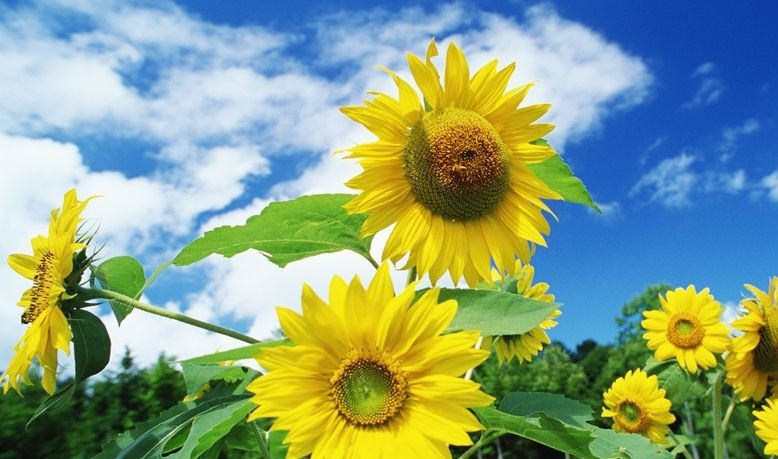
\includegraphics[width=1\textwidth]{./umetnine/soncnice.jpg}
  \caption{Tu bo neka slikica, ki bo lepa.}
  \label{fig:teaser}
\end{figure}
%

\section{Programerski del}
% TODO
% 4 STRANI SI LAHKO PRIVOŠČIMO
\chapter{Obdelava slik}\label{sec:ObdelavaSlik}
%%% Uvodni sestavek
Pri obdelavi signalov in v teoriji filtrov je Fourierova transformacija še vedno zelo močno orodje, ki se ga med drugim lahko uporablja za odstranjevanje šuma, pohitritev računanja konvolucije dveh matrik in izboljšavo kakovosti signala.

V prvem razdelku tega poglavja si bomo zato najprej pogledali teoretično ozadje za Fourierovo transformacijo in njeno izboljšano različico (hitro Fourierovo transformacijo). V našem delu se bomo ukvarjali le z obdelavo slik, zato bomo v pretežni meri vso teorijo in izpeljane postopke aplicirali na slike, čeprav bo vse skupaj v prilagojenih različicah veljalo tudi za ostale vrste signalov.

V drugem razdelku bomo nato spoznali nekaj osnovnih pojmov in postopkov iz teorije filtrov. Našteli bomo osnovne vrste transformacij slike, se naučili postopkov za njihov izračun in nato predstavili osnovne filtrirne postopke (zaznava robov na sliki, zameglitev slike, glajenje robov na sliki \ldots), ki jih bomo uporabljali v algoritmih za likovno upodabljanje slik.

V tretjem razdelku se bomo posvetili barvnim prostorom RGB, CMY, HSV in YUV. Spoznali bomo tudi Kubelka-Monk barvni model, ki ga bomo uporabili v algoritmu za likovno upodabljanje slik z voščenkami.

% TODO: Ta odstavek ni nujno resničen.
Pri obdelavi slik je postopek odstranjevanja šuma zelo pomemben, zato si bomo v zadnjem razdelku tega poglavja pogledali različne algoritme za odstranjevanje šuma. Gaussovo filtriranje je postopek za odstranjevanje šuma, ki je sicer hiter, vendar pa nam večkrat vrne nezadovoljive rezultate. Na drugi strani pa bomo spoznali še nelokalno odstranjevanje šuma s slike, ki da zelo dobre rezultate, vendar pa ima kljub temu, da lahko nekatere izračune v algoritmu pohitrimo, še vedno kvadratno časovno zahtevnost. V algoritmih za likovno upodabljanje slik bomo odvisno od naših trenutnih prioritet (hitrost ali kakovost) izbrali ustrezni postopek za odstranjevanje šuma.
%
%%%  Razdelek Fourierova transformacija.
\section{Fourierova transformacija}\label{sec:FourierT}
%
V tem razdelku bomo predstavili teorijo, ki nas bo vodila do algoritma za izračun dvodimenzionalne hitre (diskretne) Fourierove transformacije. Teorijo bomo povzeli po~\cite[2.~poglavje]{Frazier:AnIntro} in njene rezultate skupaj z dokazi zapisali za dvodimenzionalno različico ter jih opremili z lastnimi primeri. % TODO: Citiraj knjigo.
%
%% Fourierova baza.
\subsection{Fourierova baza}
%
Najprej bomo definirali $N$-dimenzionalni vektorski prostor $\l^2(\Z_N)$ nad kompleksnimi šte\-vi\-li:
$$\l^2(\Z_N) \coloneqq \set{z = (z(0), z(1), \ldots, z(N-1)) \mid z(j) \in \C, 0 \leq j \leq N-1}.$$
Prostor bomo opremili s standardno evklidsko bazo $E = \set{e_0, e_1, \ldots, e_{N-1}}$, kjer za bazni element $e_j$ velja: $e_j(n) = 1$ za $j=n$ in $e_j(n) = 0$ sicer. V nadaljevanju bomo definirali prostor $\l^2(\Z_{N_1} \times \Z_{N_2})$, ga opremili s standardno bazo in nato spoznali Fourierovo bazo.
%
\begin{definicija}
  Za naravni števili $N_1$ in $N_2$ definiramo
  $$\l^2(\Z_{N_1} \times \Z_{N_2}) \coloneqq \set{\fun{z}{\Z_{N_1} \times \Z_{N_2}}{\C}}.$$
\end{definicija}
%
Elemente $z \in \l^2(\Z_{N_1} \times \Z_{N_2})$ lahko zapišemo tudi z matriko
%
\begin{equation*}
  z =
    \begin{bmatrix}
      z(0, 0) & z(0, 1) & \hdots & z(0, N_2-1)\\
      z(1, 0) & z(1, 1) & \hdots & z(1, N_2-1)\\
      \vdots & \vdots & \ddots & \vdots\\
      z(N_1-1, 0) & z(N_1-1, 1) & \hdots & z(N_1-1, N_2-1)
    \end{bmatrix},
\end{equation*}
%
kjer so za $0 \leq n_1 \leq N_1-1, 0 \leq n_2 \leq N_2-1$ vrednosti $z(n_1, n_2) \in \C$.

Z običajnim seštevanjem in množenjem s skalarjem po komponentah postane množica $\l^2(\Z_{N_1} \times \Z_{N_2})$ vektorski prostor nad $\C$. Za elementa $z, w \in \l^2(\Z_{N_1} \times \Z_{N_2})$ definiramo kompleksni skalarni produkt
%
\begin{equation}\label{eq:defSP}
  \langle z, w\rangle \coloneqq \sum_{n_1 = 0}^{N_1 - 1} \sum_{n_2 = 0}^{N_2 - 1} z(n_1, n_2) \cdot \overline{w(n_1, n_2)} \;.
\end{equation}
%
\begin{trditev}
Prostor $\l^2(\Z_{N_1} \times \Z_{N_2})$ je $N_1 N_2$-dimenzionalen.
\end{trditev}
%
\begin{dokaz}
Dimenzija prostora je enaka razsežnosti njegove baze. Definiramo množico
$$E \coloneqq \set{e_{i,j} \mid 0 \leq i \leq N_1-1, 0 \leq j \leq N_2-1},$$
kjer je $e_{i,j}(n_1, n_2) = 1$ za $(i,j) = (n_1, n_2)$ in $e_{i,j}(n_1, n_2) = 0$ sicer. Zanjo enostavno preverimo, da je linearno neodvisna in razpenja celoten prostor $\l^2(\Z_{N_1} \times \Z_{N_2})$, torej je $N_1N_2$-razsežna baza prostora $\l^2(\Z_{N_1} \times \Z_{N_2})$.
\end{dokaz}
%
\begin{izrek}
Naj bosta $\set{B_0, B_1, \ldots, B_{N_1 - 1}}$ in $\set{C_0, C_1, \ldots, C_{N_2 - 1}}$ ortonormirani bazi za $\l^2(\Z_{N_1})$ in $\l^2(\Z_{N_2})$. Za $0 \leq m_1 \leq N_1 - 1$ in $0 \leq m_2 \leq N_2 - 1$ naj bo
$$D_{m_1, m_2}(n_1, n_2) \coloneqq B_{m_1}(n_1)C_{m_2}(n_2) \;.$$
Tedaj je $\set{D_{m_1, m_2}}_{0 \leq m_1 \leq N_1 - 1, 0 \leq m_2 \leq N_2 - 1}$ ortonormirana baza prostora $\l^2(\Z_{N_1} \times \Z_{N_2})$.
\end{izrek}
%
\begin{dokaz}
Najprej preverimo, da velja enakost $\langle D_{m_1, m_2}, D_{k_1, k_2}\rangle = \langle B_{m_1}, B_{k_1} \rangle \langle C_{m_2}, C_{k_2}\rangle$. Z uporabo definicije skalarnega produkta \eqref{eq:defSP} in s preureditvijo členov v dvojni vsoti dobimo:
%
\begin{align*}
\langle D_{m_1, m_2}, D_{k_1, k_2}\rangle & = \sum_{n_1 = 0}^{N_1 - 1} \sum_{n_2 = 0}^{N_2 - 1} D_{m_1, m_2}(n_1, n_2)\overline{D_{k_1, k_2}(n_1, n_2)} \\
& = \sum_{n_1 = 0}^{N_1 - 1} \sum_{n_2 = 0}^{N_2 - 1} B_{m_1}(n_1)C_{m_2}(n_2) \overline{B_{k_1}(n_1)C_{k_2}(n_2)} \\
& = \sum_{n_1 = 0}^{N_1 - 1} \sum_{n_2 = 0}^{N_2 - 1} B_{m_1}(n_1)\overline{B_{k_1}(n_1)}C_{m_2}(n_2) \overline{C_{k_2}(n_2)} \\
& = \sum_{n_1 = 0}^{N_1 - 1} B_{m_1}(n_1)\overline{B_{k_1}(n_1)} \sum_{n_2 = 0}^{N_2 - 1} C_{m_2}(n_2) \overline{C_{k_2}(n_2)} \\
& = \langle B_{m_1}, B_{k_1} \rangle \langle C_{m_2}, C_{k_2}\rangle.
\end{align*}
%
Z računom
$$\langle D_{m_1, m_2}, D_{k_1, k_2}\rangle = \langle B_{m_1}, B_{k_1} \rangle \langle C_{m_2}, C_{k_2}\rangle =
\begin{cases}
1 & \mbox{če } (m_1, m_2) = (k_1, k_2); \\
0 & \mbox{sicer}
\end{cases}
$$
pokažemo, da je baza $\set{D_{m_1, m_2}}_{0 \leq m_1 \leq N_1 - 1, 0 \leq m_2 \leq N_2 - 1}$ res ortonormirana (v računu uporabimo dejstvo, da sta bazi $\set{B_{m_1}}_{0 \leq m_1 \leq N_1-1}$ in $\set{C_{m_2}}_{0 \leq m_2 \leq N_2-1}$ ortonormirani).
%
\end{dokaz}
%
V vektorskem prostoru $\l^2(\Z_N)$ so ortonormirani bazni elementi za $m,n \in \set{0, \ldots, N-1}$ definirani kot
$E_m(n) \coloneqq \frac{1}{\sqrt{N}} e^{\frac{2\pi \imath mn}{N}}$.
Za $m_1 \in \set{0, \ldots, N_1-1}$ in $m_2 \in \set{0, \ldots, N_2-1}$ definiramo elemente $E_{m_1, m_2} \in \l^2(\Z_{N_1} \times \Z_{N_2})$ s formulo
$$E_{m_1, m_2}(n_1, n_2) \coloneqq \frac{1}{\sqrt{N_1N_2}} e^{\frac{2\pi \imath m_1n_1}{N_1}} e^{\frac{2\pi \imath m_2n_2}{N_2}} \;.$$
Spodnja trditev je direktna posledica zgornjega izreka.
%
\begin{trditev}
Množica $\set{E_{m_1, m_2}}_{0 \leq m_1 \leq N_1-1, 0 \leq m_2 \leq N_2-1}$ je ortonormirana baza vek\-tor\-ske\-ga prostora $\l^2(\Z_{N_1} \times \Z_{N_2})$.
\end{trditev}
%
Bazne elemente $E_{m_1, m_2}$ pomnožimo z $\frac{1}{\sqrt{N_1N_2}}$ in dobimo nove bazne elemente
$$F_{m_1, m_2}(n_1, n_2) \coloneqq \frac{1}{N_1N_2} e^{\frac{2\pi \imath m_1n_1}{N_1}} e^{\frac{2\pi \imath m_2n_2}{N_2}},$$
ki pa posledično niso več normirani.
%
\begin{definicija}
Množica $F \coloneqq \set{F_{m_1, m_2}}_{0 \leq m_1 \leq N_1 - 1, 0 \leq m_2 \leq N_2 - 1}$ je \emph{Fourierova baza} prostora $\l^2(\Z_{N_1} \times \Z_{N_2})$.
\end{definicija}
%
Z uporabo zveze $e^{\imath \varphi} = \cos \varphi + \imath \cdot \sin \varphi$ lahko Fourierove bazne elemente zapišemo še na drug način s formulo
$$F_{m_1, m_2}(n_1, n_2) = \frac{1}{N_1N_2} \left(\cos\left[2\pi \left(\frac{m_1 n_1}{N_1} + \frac{m_2 n_2}{N_2}\right)\right] + \imath \sin\left[2\pi \left(\frac{m_1 n_1}{N_1} + \frac{m_2 n_2}{N_2}\right)\right] \right) \;.$$
%
\begin{primer}
Fourierova baza prostora $\l^2(\Z_2 \times \Z_3)$ je množica
$$F = \{F_{0,0}, F_{0,1}, F_{0,2}, F_{1,0}, F_{1,1}, F_{1,2}\},$$
kjer so bazni elementi enaki:\\[0.2cm]
%
\begin{tabular}{ll}
  $
  F_{0,0} = \frac{1}{6}\cdot
    \begin{bmatrix}
      1 & 1 & 1\\
      1 & 1 & 1
    \end{bmatrix},
  $ &
  $
  F_{1,0} = \frac{1}{6}\cdot
    \begin{bmatrix}
      1 & 1 & 1\\
      -1 & -1 & -1
    \end{bmatrix},
  $ \\[0.3cm]
  $
  F_{0,1} = \frac{1}{6}\cdot
    \begin{bmatrix}
      1 & -\frac{1}{2}+\frac{\imath \sqrt{3}}{2} & -\frac{1}{2}-\frac{\imath \sqrt{3}}{2} \\[0.1cm]
      1 & -\frac{1}{2}+\frac{\imath \sqrt{3}}{2} & -\frac{1}{2}-\frac{\imath \sqrt{3}}{2}
    \end{bmatrix},
  $ &
  $
  F_{1,1} = \frac{1}{6}\cdot
    \begin{bmatrix}
      1 & -\frac{1}{2}+\frac{\imath \sqrt{3}}{2} & -\frac{1}{2}-\frac{\imath \sqrt{3}}{2} \\[0.1cm]
      -1 & \frac{1}{2}-\frac{\imath \sqrt{3}}{2} & \frac{1}{2}+\frac{\imath \sqrt{3}}{2}
    \end{bmatrix},
  $ \\[0.3cm]
  $
  F_{0,2} = \frac{1}{6}\cdot
    \begin{bmatrix}
      1 & -\frac{1}{2}-\frac{\imath \sqrt{3}}{2} & -\frac{1}{2}+\frac{\imath \sqrt{3}}{2} \\[0.1cm]
      1 & -\frac{1}{2}-\frac{\imath \sqrt{3}}{2} & -\frac{1}{2}+\frac{\imath \sqrt{3}}{2}
    \end{bmatrix},
  $ &
  $
  F_{1,2} = \frac{1}{6}\cdot
    \begin{bmatrix}
      1 & -\frac{1}{2}-\frac{\imath \sqrt{3}}{2} & -\frac{1}{2}+\frac{\imath \sqrt{3}}{2} \\[0.1cm]
      -1 & \frac{1}{2}+\frac{\imath \sqrt{3}}{2} & \frac{1}{2}-\frac{\imath \sqrt{3}}{2}
    \end{bmatrix}.
  $
\end{tabular}

  \hfill $\lozenge$
%
\end{primer}
%
%%
\subsection{Dvodimenzionalna diskretna Fourierova transformacija}
\emph{Dvodimenzionalna diskretna Fourierova transformacija} (kratica 2DFT) je preslikava
$$\fun{\F}{\l^2(\Z_{N_1} \times \Z_{N_2})}{\l^2(\Z_{N_1} \times \Z_{N_2})},$$
ki je za $z \in \l^2(\Z_{N_1} \times \Z_{N_2})$ definirana s formulo
$$\F(z)(m_1, m_2) \coloneqq \sum_{n_1 = 0}^{N_1 - 1} \sum_{n_2 = 0}^{N_2 - 1} z(n_1, n_2) e^{\frac{-2\pi \imath m_1n_1}{N_1}} e^{\frac{-2\pi \imath m_2n_2}{N_2}} \;.$$
\emph{Dvodimenzionalna diskretna inverzna Fourierova transformacija} (kratica 2IFT) je preslikava
$$\fun{\F^{-1}}{\l^2(\Z_{N_1} \times \Z_{N_2})}{\l^2(\Z_{N_1} \times \Z_{N_2})},$$
ki je za $w \in \l^2(\Z_{N_1} \times \Z_{N_2})$ definirana s formulo
$$\F^{-1}(w)(n_1, n_2) \coloneqq \frac{1}{N_1 N_2} \sum_{m_1 = 0}^{N_1 - 1} \sum_{m_2 = 0}^{N_2 - 1} w(m_1, m_2) e^{\frac{2\pi \imath m_1n_1}{N_1}} e^{\frac{2\pi \imath m_2n_2}{N_2}} \;.$$
%
Enostavno lahko preverimo, da sta zgornji preslikavi dobro definirani in res slikata nazaj v isti prostor.

Ker je $\set{E_{m_1, m_2}}_{0 \leq m_1 \leq N_1 - 1, 0 \leq m_2 \leq N_2 - 1}$ ortonormirana baza, lahko $z \in \l^2(\Z_{N_1} \times \Z_{N_2})$ razvijemo po tej bazi kot
\begin{equation}\label{eq:razvojE}
z = \sum_{m_1 = 0}^{N_1 - 1} \sum_{m_2 = 0}^{N_2 - 1} \langle z, E_{m_1, m_2} \rangle E_{m_1, m_2} \;.
\end{equation}
Pri tem je
\begin{equation}\label{eq:skalarE}
\langle z, E_{m_1, m_2}\rangle = \sum_{n_1 = 0}^{N_1 - 1} \sum_{n_2 = 0}^{N_2 - 1} z(n_1, n_2) \overline{\frac{1}{\sqrt{N_1N_2}} e^{\frac{2\pi \imath m_1n_1}{N_1}} e^{\frac{2\pi \imath m_2n_2}{N_2}}} \;.
\end{equation}
%
S pomočjo tega razvoja bomo preprosto pokazali, da velja naslednja trditev.
%
%TODO Tu ni v redu. Povej kaj v kerem enačaju uporabiš.
\begin{trditev}\label{trd:obratnoLevo}
Za vsak $z \in \l^2(\Z_{N_1} \times \Z_{N_2})$ velja:
$$z = (\F^{-1}\F)(z).$$
\end{trditev}
%
\begin{dokaz}
Z upoštevanjem formul \eqref{eq:razvojE} in \eqref{eq:skalarE} naredimo naslednji izračun:
%
\begin{align*}
 & (\F^{-1} \F)(z)(k_1, k_2) = \\
 & = \frac{1}{N_1N_2} \sum_{m_1 = 0}^{N_1 - 1} \sum_{m_2 = 0}^{N_2 - 1} \left(\sum_{n_1 = 0}^{N_1 - 1} \sum_{n_2 = 0}^{N_2 - 1} z(n_1, n_2) e^{\frac{-2\pi \imath m_1n_1}{N_1}} e^{\frac{-2\pi \imath m_2n_2}{N_2}}\right) e^{\frac{2\pi \imath k_1m_1}{N_1}} e^{\frac{2\pi \imath k_2m_2}{N_2}} \\
 & = \sum_{m_1 = 0}^{N_1 - 1} \sum_{m_2 = 0}^{N_2 - 1} \left(\sum_{n_1 = 0}^{N_1 - 1} \sum_{n_2 = 0}^{N_2 - 1} z(n_1, n_2) \frac{1}{\sqrt{N_1N_2}} e^{\frac{-2\pi \imath m_1n_1}{N_1}} e^{\frac{-2\pi \imath m_2n_2}{N_2}}\right) \frac{1}{\sqrt{N_1N_2}} e^{\frac{2\pi \imath k_1m_1}{N_1}} e^{\frac{2\pi \imath k_2m_2}{N_2}} \\
 & = \sum_{m_1 = 0}^{N_1 - 1} \sum_{m_2 = 0}^{N_2 - 1} \langle z, E_{m_1, m_2} \rangle E_{m_1, m_2}(k_1, k_2) = z(k_1, k_2) \;.
\end{align*}
%
Ker ta izračun velja za vsak par $(k_1, k_2) \in \l^2(\Z_{N_1} \times \Z_{N_2})$, je trditev s tem dokazana.
\end{dokaz}
%
\begin{primer}\label{pri:obrat}
Naj bo $z \in \l^2(\Z_{2} \times \Z_{3})$, npr.
%
$$z = \begin{bmatrix}
      3\imath & 10 & 10 - \imath\\
      2 & 0 & -\imath
    \end{bmatrix}.$$
%
Na tem primeru bomo sedaj preverili, da velja trditev \ref{trd:obratnoLevo}. Za vsak par $(m_1, m_2) \in \Z_{2} \times \Z_{3}$ izračunamo vrednost $\F(z)(m_1, m_2)$ in dobimo matriko
%
$$  \F(z) = w = 
    \begin{bmatrix}
      22+\imath & -8 + \sqrt{3} +4\imath & -8 - \sqrt{3} +4\imath \\[0.1cm]
      18+3\imath & -12 + 3\imath & -12+3\imath
    \end{bmatrix}\;.$$
%
Če na matriki $w$ sedaj uporabimo 2IFT, dobimo nazaj matriko $z$. Torej res velja $z = (\F^{-1}\F)(z)$. \hfill $\lozenge$
\end{primer}
%
Bolj kot razvoj po standardni bazi bo za nas zanimiv razvoj po Fourierovi bazi. Iz izračuna v zadnjem dokazu je razvidno, da je
\begin{align}\label{eq:primerjava}
z = \sum_{m_1 = 0}^{N_1 - 1} \sum_{m_2 = 0}^{N_2 - 1} \left(\sum_{n_1 = 0}^{N_1 - 1} \sum_{n_2 = 0}^{N_2 - 1} z(n_1, n_2) \frac{1}{\sqrt{N_1N_2}} e^{\frac{-2\pi \imath m_1n_1}{N_1}} e^{\frac{-2\pi \imath m_2n_2}{N_2}}\right) E_{m_1, m_2}.
\end{align}
%
S preureditvijo členov in uporabo definicije Fourierove baze dobimo, da je
\begin{align*}
z & = \sum_{m_1 = 0}^{N_1 - 1} \sum_{m_2 = 0}^{N_2 - 1} \left(\sum_{n_1 = 0}^{N_1 - 1} \sum_{n_2 = 0}^{N_2 - 1} z(n_1, n_2) e^{\frac{-2\pi \imath m_1n_1}{N_1}} e^{\frac{-2\pi \imath m_2n_2}{N_2}}\right) F_{m_1,m_2} \\
& = \sum_{m_1 = 0}^{N_1 - 1} \sum_{m_2 = 0}^{N_2 - 1} \F(z)(m_1, m_2) F_{m_1, m_2}.
\end{align*}
%
Kadar $z$ razvijemo po Fourierovi bazi, pravimo, da smo ga zapisali v \emph{frekvenčni domeni}.\footnote{V razdelku \ref{sec:globT} bomo videli fizikalno interpretacijo zapisa v Fourierovi bazi in naredili njihovo vizualno predstavitev.} %TODO Opombo popravi.
%
\begin{primer}
Element $z$ iz primera~\ref{pri:obrat},
%
$$z = \begin{bmatrix}
      3\imath & 10 & 10 - \imath\\
      2 & 0 & -\imath
    \end{bmatrix},$$
%
bomo zapisali v Fourierovi bazi:
\begin{multline*}
z = (22+\imath) \cdot F_{0,0} + (-8 + \sqrt{3} +4\imath) \cdot F_{0,1} + (-8 - \sqrt{3} +4\imath) \cdot F_{0,2} + \\
+ (18+3\imath) \cdot F_{1,0} + (-12 + 3\imath) \cdot F_{1,1}+ (-12+3\imath) \cdot F_{1,2},
\end{multline*}
kjer so $F_{n_1, n_2}$ Fourierovi bazni elementi prostora $\l^2(\Z_2 \times \Z_3)$.
\hfill $\lozenge$
\end{primer}
%
\begin{izrek}
Za $z, w \in \l^2(\Z_{N_1} \times \Z_{N_2})$ veljata naslednji dve formuli:
\begin{enumerate}
\item Parsevalova formula:
$$\langle z, w \rangle = \frac{1}{N_1 N_2} \langle \F(z), \F(w) \rangle;$$
\item Plancherelova formula:
$$\norm{z}^2 = \frac{1}{N_1 N_2} \norm{\F(z)}^2.$$
\end{enumerate}
\end{izrek}
%
\begin{dokaz} Najprej bomo dokazali Parsevalovo formulo. S primerjavo formul \eqref{eq:razvojE} in \eqref{eq:primerjava} opazimo, da velja $\F(z(m_1, m_2)) = \sqrt{N_1N_2} \cdot \langle z, E_{m_1, m_2}\rangle$. Z uporabo te ugotovitve in formule \eqref{eq:defSP} za izračun skalarnega produkta dobimo, da je
%
\begin{align*}
\langle z, w \rangle & = \sum_{n_1 = 0}^{N_1 - 1} \sum_{n_2 = 0}^{N_2 - 1} z(n_1, n_2) \cdot \overline{w(n_1, n_2)} \\
& = \sum_{n_1 = 0}^{N_1 - 1} \sum_{n_2 = 0}^{N_2 - 1} \frac{1}{\sqrt{N_1N_2}} \F(z(n_1, n_2)) \frac{1}{\sqrt{N_1N_2}} \F(w(n_1,n_2)) \;.
\end{align*}
% 
S tem smo pokazali veljavnost Parsevalove formule. Plancherelovo formulo enostavno dokažemo tako, da ponovimo postopek za $w = z$ in uporabimo definicijo norme.
\end{dokaz}
%
\subsection{Translacijsko invariantne linearne transformacije}
\emph{Transformacija} je matematični zapis sistema, ki poskrbi za pretvorbo vhodnega signala v izhodnega. Sistemi, ki jih modeliramo s transformacijo, so običajno linearni (pripadajoča transformacija je linearna) in invariantni (v primeru časovno ali prostorsko zamaknjenega vhodnega signala, ima te lastnosti tudi izhodni signal). V našem delu bomo modelirali sivinske slike, zato se bomo sedaj osredotočili na dvodimenzionalne transformacije.
 
Naj bo sedaj $z$ zaporedje, ki ga definiramo na množici $\Z \times \Z$ (elementi zaporedja so $z(n_1,n_2) \in \C$ za $(n_1,n_2) \in \Z \times \Z$). Za zaporedje $z$ pravimo, da je \emph{periodično} v prvi spremenljivki s periodo $N_1$ in v drugi spremenljivki s periodo $N_2$, če za vse $n_1, n_2, j_1, j_2 \in \Z$ velja
$$z(n_1 + j_1 N_1, n_2 + j_2 N_2) = z(n_1, n_2) \;.$$
%
\begin{definicija}
Za $k_1, k_2 \in \Z$ je \emph{translacijsko invariantna linearna transformacija}
$$\fun{R_{k_1, k_2}}{\l^2(\Z_{N_1} \times \Z_{N_2})}{\l^2(\Z_{N_1} \times \Z_{N_2})}$$
definirana s formulo
$$(R_{k_1, k_2}z)(n_1, n_2) \coloneqq z(n_1 - k_1, n_2 - k_2) \;.$$
\end{definicija}
%
Pravimo, da je transformacija $\fun{T}{\l^2(\Z_{N_1} \times \Z_{N_2})}{\l^2(\Z_{N_1} \times \Z_{N_2})}$ \emph{translacijsko invariantna}, če za vse $k_1, k_2 \in \Z$ in $z \in \l^2(\Z_{N_1} \times \Z_{N_2})$ velja:
$$T(R_{k_1, k_2} z) = R_{k_1, k_2} T(z).$$
%
\begin{trditev}
Če je transformacija $\fun{T}{\l^2(Z_{N_1} \times Z_{N_2})}{\l^2(Z_{N_1} \times Z_{N_2})}$ translacijsko invariantna, tedaj za vsak Fourierov bazni element $F_{m_1, m_2}$ velja, da je lastni vektor transformacije $T$.
\end{trditev}
%
\begin{dokaz}
Naj bo $F_{m_1, m_2}$ Fourierov bazni element v prostoru $\l^2(Z_{N_1} \times Z_{N_2})$. Ker je $F$ baza prostora $\l^2(Z_{N_1} \times Z_{N_2})$, obstajajo taka kompleksna števila $\{a_{i, j}\}_{i, j = 0}^{i = N_1 - 1, j = N_2 - 1}$, da za vsak par $(n_1, n_2) \in \N \times \N$ velja:
%
\begin{align}\label{eq:transformacija} %TODO označitev - vsaka vrstica posebaj ??
  T(F_{m_1, m_2})(n_1, n_2) & = \sum_{k_1=0}^{N_1-1} \sum_{k_2=0}^{N_2-1} a_{k_1, k_2} F_{k_1, k_2}(n_1, n_2) \\
 & = \frac{1}{N_1N_2} \sum_{k_1=0}^{N_1-1} \sum_{k_2=0}^{N_2-1} a_{k_1, k_2} e^{\frac{2\pi \imath k_1n_1}{N_1}} e^{\frac{2\pi \imath k_2n_2}{N_2}}.
\end{align}
%
Po definiciji preslikave $R_{k_1, k_2}$ velja:
%
\begin{align*}
(R_{1, 0} F_{m_1, m_2})(n_1, n_2) & = F_{m_1, m_2}(n_1-1, n_2) = \frac{1}{N_1N_2} e^{\frac{2\pi \imath m_1(n_1-1)}{N_1}} e^{\frac{2\pi \imath m_2n_2}{N_2}} \\
& = \frac{1}{N_1N_2} e^{-\frac{2\pi \imath m_1}{N_1}} e^{\frac{2\pi \imath m_1n_1}{N_1}} e^{\frac{2\pi \imath m_2n_2}{N_2}} \\
& =  e^{-\frac{2\pi \imath m_1}{N_1}} F_{m_1, m_2}(n_1, n_2) \;.
\end{align*}
%
Ker je $T$ linearna preslikava in je člen $e^{-\frac{2\pi \imath m_1}{N_1}}$ neodvisen od spremenljivk $n_1$ in $n_2$, z nadaljno uporabo enačbe \eqref{eq:transformacija}, velja:
%
\begin{align*}
T(R_{1, 0} F_{m_1, m_2})(n_1, n_2) & = e^{-\frac{2\pi \imath m_1}{N_1}} T(F_{m_1, m_2})(n_1, n_2) \\
& = e^{-\frac{2\pi \imath m_1}{N_1}} \frac{1}{N_1N_2} \sum_{k_1=0}^{N_1-1} \sum_{k_2=0}^{N_2-1} a_{k_1, k_2} e^{\frac{2\pi \imath k_1n_1}{N_1}} e^{\frac{2\pi \imath k_2n_2}{N_2}} \\
& =  \sum_{k_1=0}^{N_1-1} \sum_{k_2=0}^{N_2-1} e^{-\frac{2\pi \imath m_1}{N_1}} a_{k_1, k_2} F_{k_1, k_2}(n_1, n_2) \;.
\end{align*}
%
Dobili smo razvoj $T(R_{1, 0} F_{m_1, m_2})(n_1, n_2)$ po Fourierovi bazi. Sedaj bomo s pomočjo \eqref{eq:transformacija} razvili po Fourierovi bazi še $(R_{1, 0} T(F_{m_1, m_2}))(n_1, n_2)$:
%
\begin{align*}
R_{1, 0} (T(F_{m_1, m_2}))(n_1, n_2) & = T(F_{m_1, m_2})(n_1-1, n_2) \\
& = \frac{1}{N_1N_2} \sum_{k_1=0}^{N_1-1} \sum_{k_2=0}^{N_2-1} a_{k_1, k_2} e^{\frac{2\pi \imath k_1(n_1-1)}{N_1}} e^{\frac{2\pi \imath k_2n_2}{N_2}} \\
& = \sum_{k_1=0}^{N_1-1} \sum_{k_2=0}^{N_2-1} a_{k_1, k_2} e^{-\frac{2\pi \imath k_1}{N_1}} F_{k_1, k_2}(n_1, n_2) \;.
\end{align*}
%
Ker smo predpostavili, da je $T$ translacijsko invariantna transformacija, za vsak par $(n_1, n_2) \in \Z \times \Z$ velja, da je $T(R_{1, 0} (F_{m_1, m_2}))(n_1, n_2) = R_{1, 0}(T(F_{m_1, m_2}))(n_1, n_2)$. Zaradi enoličnosti razvoja po bazi sledi, da morajo biti koeficienti v zgornjih dveh razvojih enaki. Za vsak par $(k_1, k_2) \in \Z_{N_1} \times \Z_{N_2}$ velja:
%
\begin{equation*}
a_{k_1, k_2} e^{-\frac{2\pi im_1}{N_1}} = a_{k_1, k_2} e^{-\frac{2\pi \imath k_1}{N_1}}.
\end{equation*} 
%
Za $k_1 \neq m_1$, velja $e^{-\frac{2\pi \imath m_1}{N_1}} \neq e^{-\frac{2\pi \imath k_1}{N_1}}$, ker je $0 \leq k_1, m_1 \leq N_1-1$. Če želimo, da velja enakost v zgornji enačbi, mora biti za $k_1 \neq m_1$ koeficient $a_{k_1, k_2} = 0$.

Podobno bi dobili, da mora biti za $k_2 \neq m_2$ koeficient $a_{k_1, k_2} = 0$, če bi v zgornjih izračunih namesto $R_{1, 0}$ vzeli $R_{0, 1}$. Dobili smo, da mora biti za $(k_1, k_2) \neq (m_1, m_2)$ koeficient $a_{k_1, k_2} = 0$. V enačbi \eqref{eq:transformacija} zato odpadejo vsi členi, razen tistega pri $(k_1, k_2) = (m_1, m_2)$. Dobimo, da je $T(F_{m_1, m_2})(n_1, n_2) = a_{m_1, m_2}F_{m_1, m_2}(n_1, n_2)$ oz.\ 
$$T(F_{m_1, m_2}) = a_{m_1, m_2}F_{m_1, m_2},$$
kar dokazuje, da je $F_{m_1, m_2}$ lastni vektor transformacije $T$ z lastno vrednostjo $a_{m_1, m_2}$. S tem je dokazana celotna trditev, saj smo to dokazali za splošen $F_{m_1, m_2}$.
\end{dokaz}
%
\begin{posledica}
Translacijsko invariantne linearne transformacije $T$ so dia\-go\-na\-li\-za\-bil\-ne v Fourierovi bazi.
\end{posledica}
%
Zgornja posledica enostavno sledi iz ravnokar dokazane trditve. V nadaljevanju bomo definirali operator $\ast$, na podlagi katerega bomo znali hitro izračunati FFT kasneje ob uporabi te posledice. % TODO nujno popravi tole
%
\begin{definicija}
Za vse $z, w \in \l^2(\Z_{N_1} \times \Z_{N_2})$ in $(m_1, m_2) \in \Z_{N_1} \times \Z_{N_2}$ definiramo operator $z \ast w \in \l^2(\Z_{N_1} \times \Z_{N_2})$ s formulo
$$z \ast w(m_1, m_2) \coloneqq \sum_{n_1 = 0}^{N_1 - 1} \sum_{n_2 = 0}^{N_2 - 1} z(m_1 - n_1, m_2 - n_2)w(n_1, n_2) \;.$$
\end{definicija}
%
\begin{primer}
Naj bosta
$z = \left(\begin{smallmatrix}
  1 & 1\\
  0 & \imath
\end{smallmatrix} \right)$
in
$w = \left(\begin{smallmatrix}
  \imath & 0\\
  1 & \imath
\end{smallmatrix} \right)$
elementa prostora $\l^2(\Z_2 \times \Z_2)$. Z upoštevanjem periodičnosti izračunamo
%
\begin{align*}
z \ast w(0, 0) & = \sum_{n_1 = 0}^1 \sum_{n_2 = 0}^1 z(- n_1, - n_2) w(n_1, n_2) \\
& = z(0, 0) w(0, 0) + z(0, -1) w(0, 1) + z(-1, 0) w(1, 0)+ z(-1, -1) w(1, 1) \\
& = z(0, 0) w(0, 0) + z(0, 1) w(0, 1) + z(1, 0) w(1, 0)+ z(1, 1) w(1, 1) \\
& = 1 \cdot \imath + 1 \cdot 0 + 0 \cdot 1 + \imath \cdot \imath = -1 + \imath.
\end{align*}
%
Podobno izračunamo preostale tri vrednosti:
%
\begin{align*}
z \ast w(0, 1) & = \sum_{n_1 = 0}^1 \sum_{n_2 = 0}^1 z(- n_1, 1 - n_2) w(n_1, n_2) = 1 \cdot \i + 1 \cdot 0 + \i \cdot 1 + 1 \cdot \i = 3\i, \\
z \ast w(1, 0) & = \sum_{n_1 = 0}^1 \sum_{n_2 = 0}^1 z(1 - n_1, - n_2) w(n_1, n_2) = 0 \cdot \i + \i \cdot 0 + 1 \cdot 1 + 1 \cdot \i = 1 + \i, \\
z \ast w(1, 1) & = \sum_{n_1 = 0}^1 \sum_{n_2 = 0}^1 z(1 - n_1, 1 - n_2) w(n_1, n_2) = \i \cdot \i + 0 \cdot 0 + 1 \cdot 1 + 1 \cdot \i = \i.
\end{align*}
%
Torej je
$z \ast w = \left(\begin{smallmatrix}
  -1 + \i & 3\i\\
  1 + \i & \i
\end{smallmatrix} \right)$. \hfill $\lozenge$
\end{primer}
%
\begin{izrek}
Veljajo naslednje trditve:
\begin{enumerate}
\item Za vse $(m_1, m_2) \in \Z \times \Z$ velja
$$\F(z \ast w)(m_1, m_2) = \F(z)(m_1, m_2) \F(w)(m_1, m_2).$$
\item Za $b \in \l^2(\Z_{N_1} \times \Z_{N_2})$ definiramo $\fun{T_b}{\l^2(\Z_{N_1} \times \Z_{N_2})}{\l^2(\Z_{N_1} \times \Z_{N_2})}$ z
$$T_b(z) = b \ast z.$$
Vsaki linearni transformaciji te oblike pravimo, da je \emph{konvolucijski operator}. Velja, da je $T_b$ translacijsko invariantna preslikava.
\item Za $m \in \l^2(\Z_{N_1} \times \Z_{N_2})$ definiramo $\fun{T_{(m)}}{\l^2(\Z_{N_1} \times \Z_{N_2})}{\l^2(\Z_{N_1} \times \Z_{N_2})}$ kot
$$T_{(m)}(z) = \F^{-1}(m\F(z)),$$
kjer je za vsak $(n_1, n_2)$ $(m\F(z))(n_1, n_2) = m(n_1, n_2) \cdot \F(z)(n_1, n_2)$. Vsaki linearni transformaciji takega tipa pravimo, da je \emph{Fourierov multiplikativni operator}. Velja, da je vsak konvolucijski operator $T_b$, pri izbiri $m = \F(b)$, enak Fourierovemu multiplikativnemu operatorju $T_{(m)}$.
\end{enumerate}
\end{izrek}
%
\begin{dokaz} (1) Z uporabo definicij Fourierove transformacije in konvolucije naredimo naslednji izračun:
%
\begin{align*}
&\F(z \ast w)(m_1, m_2) = \\
& = \sum_{n_1 = 0}^{N_1 - 1} \sum_{n_2 = 0}^{N_2 - 1} z \ast w(n_1, n_2) e^{\frac{-2\pi \imath m_1n_1}{N_1}} e^{\frac{-2\pi \imath m_2n_2}{N_2}} \\
& = \sum_{n_1 = 0}^{N_1 - 1} \sum_{n_2 = 0}^{N_2 - 1} \sum_{k_1 = 0}^{N_1 - 1} \sum_{k_2 = 0}^{N_2 - 1} z(n_1 - k_1, n_2 - k_2) w(k_1, k_2) e^{\frac{-2\pi \imath m_1n_1}{N_1}} e^{\frac{-2\pi \imath m_2n_2}{N_2}} \\
& = \sum_{n_1 = 0}^{N_1 - 1} \sum_{n_2 = 0}^{N_2 - 1} \sum_{k_1 = 0}^{N_1 - 1} \sum_{k_2 = 0}^{N_2 - 1} z(n_1 - k_1, n_2 - k_2) w(k_1, k_2) e^{\frac{-2\pi \imath m_1(n_1-k_1)}{N_1}} e^{\frac{-2\pi \imath m_2(n_2-k_2)}{N_2}} e^{\frac{-2\pi \imath m_1k_1}{N_1}} e^{\frac{-2\pi \imath m_2k_2}{N_2}} \\
& = \sum_{k_1 = 0}^{N_1 - 1} \sum_{k_2 = 0}^{N_2 - 1} w(k_1, k_2) e^{\frac{-2\pi \imath m_1k_1}{N_1}} e^{\frac{-2\pi \imath m_2k_2}{N_2}} \sum_{n_1 = 0}^{N_1 - 1} \sum_{n_2 = 0}^{N_2 - 1} z(n_1 - k_1, n_2 - k_2) e^{\frac{-2\pi \imath m_1(n_1-k_1)}{N_1}} e^{\frac{-2\pi \imath m_2(n_2-k_2)}{N_2}}.
\end{align*}
%
Zadnjo dvojno vsoto z uvedbo novih spremenljivk $l_1 = n_1 - k_1$ in $l_2 = n_2 - k_2$ prevedemo v:
%
\begin{align*}
\sum_{n_1 = 0}^{N_1 - 1} \sum_{n_2 = 0}^{N_2 - 1} & z(n_1 - k_1, n_2 - k_2) e^{\frac{-2\pi \imath m_1(n_1-k_1)}{N_1}} e^{\frac{-2\pi \imath m_2(n_2-k_2)}{N_2}} = \\
& = \sum_{l_1 = -k_1}^{N_1 - 1 - k_1} \sum_{l_2 = -k_2}^{N_2 - 1 - l_2} z(l_1, l_2) e^{\frac{-2\pi \imath m_1l_1}{N_1}} e^{\frac{-2\pi \imath m_2l_2}{N_2}} \\
& = \sum_{l_1 = 0}^{N_1 - 1} \sum_{l_2 = 0}^{N_2 - 1} z(n_1 - k_1, n_2 - k_2) e^{\frac{-2\pi \imath m_1l_1}{N_1}} e^{\frac{-2\pi \imath m_2l_2}{N_2}} \;.
\end{align*}
%
V zadnjem enačaju smo uporabili, da sta izraza v vsoti periodična s periodo $N_1$ oz.\ $N_2$. Z uvedbo novih spremenljivk dobimo:
%
\begin{align*}
\F(z \ast w)& (m_1, m_2) = \\
& = \sum_{k_1 = 0}^{N_1 - 1} \sum_{k_2 = 0}^{N_2 - 1} w(k_1, k_2) e^{\frac{-2\pi \imath m_1k_1}{N_1}} e^{\frac{-2\pi \imath m_2k_2}{N_2}} \sum_{l_1 = 0}^{N_1 - 1} \sum_{l_2 = 0}^{N_2 - 1} z(l_1, l_2) e^{\frac{-2\pi \imath m_1l_1}{N_1}} e^{\frac{-2\pi \imath m_2l_2}{N_2}} \\
& = \F(z)(m_1, m_2) \F(w)(m_1, m_2),
\end{align*}
%
kar dokazuje prvo točko izreka, saj zgornje velja za poljubna $m_1$ in $m_2$.

(2) Naj bo $z \in \l^2(\Z_{N_1} \times \Z_{N_2})$ in $(k_1, k_2) \in \Z \times \Z$. Tedaj za vsak par $(k_1, k_2) \in \Z_{N_1} \times \Z_{N_2}$ velja naslednji izračun:
%
\begin{align*}
T_b(R_{k_1, k_2}z)(m_1, m_2) & = b \ast (R_{k_1, k_2}z)(m_1, m_2) \\
& =  \sum_{n_1 = 0}^{N_1 - 1} \sum_{n_2 = 0}^{N_2 - 1} b(m_1 - n_1, m_2 - n_2) (R_{k_1, k_2}z)(n_1, n_2) \\
& =  \sum_{n_1 = 0}^{N_1 - 1} \sum_{n_2 = 0}^{N_2 - 1} b(m_1 - n_1, m_2 - n_2) z(n_1 - k_1, n_2 - k_2) \;.
\end{align*}
%
Z uvedbo novih spremenljivk $l_1 = n_1 - k_1$ in $l_2 = n_2 - k_2$ v zadnji vsoti in upoštevanjem periodičnosti, za vsak par $(m_1, m_2) \in \Z \times \Z$ velja
%
\begin{align*}
T_b(R_{k_1, k_2}z)(m_1, m_2) & = \\
& = \sum_{l_1 = -k_1}^{N_1 - 1 - k_1} \sum_{l_2 = -k_2}^{N_2 - 1 - k_2} b(m_1 - k_1 - l_1, m_2 - k_2 - l_2) z(l_1, l_2) \\
& = \sum_{l_1 = 0}^{N_1 - 1} \sum_{l_2 = 0}^{N_2 - 1} b(m_1 - k_1 - l_1, m_2 - k_2 - l_2) z(l_1, l_2) \\
& = (b \ast z)(m_1 - k_1, m_2 - k_2) \\
& = R_{k_1, k_2}(b \ast z)(m_1, m_2) \\
& = R_{k_1, k_2}T_b(z)(m_1, m_2).
\end{align*}
%
S tem smo pokazali, da je $T_b(R_{k_1, k_2}z) = R_{k_1, k_2}T_b(z)$, tj.\ $T_b$ je res translacijski operator.

(3) Z uporabo prve točke tega izreka in definicije inverzne Fourierove transformacije za vsak $z \in \l^2(\Z_{N_1} \times \Z_{N_2})$ izračunamo:
%
\begin{equation*}
T_b(z) = b \ast z = \F^{-1}(b \ast z) = \F^{-1}(\F(b) \F(z)) = \F^{-1}(m \F(z)) = T_{(m)}(z),
\end{equation*}
%
kar dokazuje tretjo točko izreka.
\end{dokaz}
%
Od tod sledi naslednji izrek, v katerem smo dokazali, ostale implikacije pa sledijo enostavno. %TODO popravi to pa premisli
%
\begin{izrek}
Naj bo $\fun{T}{\l^2(\Z_{N_1} \times \Z_{N_2})}{\l^2(\Z_{N_1} \times \Z_{N_2})}$ linearna transformacija. Naslednje trditve so ekvivalentne:
%
\begin{enumerate}
  \item $T$ je translacijsko invariantni operator;
  \item $T$ je Fourierov multiplikativni operator;
  \item $T$ je konvolucijski operator.
\end{enumerate}
%
\end{izrek}
%%
\subsection{Hitra Fourierova transformacija}
V tem podrazdelku bomo razvili algoritem za dvodimenzionalno hitro diskretno Fouriero\-vo transformacijo.
Naj bo $z \in \l^2(\Z_{N_1} \times \Z_{N_2})$. Za izračun $\F(z)(m_1, m_2)$ potrebujemo $N_1 N_2$ kompleksnih množenj.\footnote{Šteli bomo le kompleksna množenja. Operacij seštevanja ne bomo šteli. Število realnih množenj je potem trikrat večje, saj za množenje dveh kompleksnih števil potrebujemo tri realna množenja: $(a + b \imath)(c + d\imath) = (a - b)d + (c - d)a + [(a - b)d + (c + d)b]\imath$.} Za celotni izračun $\F(z)$ torej potrebujemo $N_1^2 N_2^2$ kompleksnih množenj.

Če razpišemo izračun za $\F(z)$, opazimo, da se nekateri členi v njej večkrat ponovijo. V naslednji trditvi bomo izkoristili to ugotovitev in s tem zmanjšali potrebno število kompleksnih množenj za izračun rezultata.
%
\begin{trditev} \label{trd:2dft}
Naj bo
$$y(n_1, m_2) \coloneqq \sum_{n_2 = 0}^{N_2 - 1} z(n_1, n_2) e^{-\frac{2\pi \imath m_2n_2}{N_2}}.$$
Tedaj lahko Fourierovo transformacijo zapišemo kot
$$\F(z)(m_1, m_2) = \sum_{n_1 = 0}^{N_1 - 1} y(n_1, m_2) e^{-\frac{2\pi \imath m_1n_1}{N_1}}.$$
Za izračun 2DFT potrebujemo $N_1 N_2 (N_1 + N_2)$ kompleksnih množenj.
\end{trditev}
%
\begin{dokaz}
Za izračun $y(n_1, m_2)$ potrebujemo $N_2$ kompleksnih množenj. Skupno, za vse možne pare $(n_1, m_2)$, torej potrebujemo $(N_1 N_2)\cdot N_2$ kompleksnih množenj. Pri izračunu $\F(z)(m_1, m_2)$ upoštevamo, da je vrednost $y(n_1, m_2)$ že znana. Torej za njen izračun potrebujemo $N_1$ komplesknih množenj. Za vse možne kombinacije $(m_1, m_2)$ skupaj potrebujemo $(N_1 N_2) \cdot N_1$ kompleksnih množenj.

Celotni izračun 2DFT torej zahteva $N_1 N_2 (N_1 + N_2)$ kompleksnih množenj. 
\end{dokaz}
%
Zgornje število kompleksnih množenj lahko še zmanjšamo. V zgornji trditvi smo izračun 2DFT prevedli na zaporedni izračun dveh enodimenzionalnih DFT. Za vsakega izmed teh izračunov torej potrebujemo največ toliko kompleksnih množenj kot jih zahteva izračun 1DFT. Izkaže se, da lahko v nekaterih primerih izračun 1DFT zelo pohitrimo, o tem se bomo prepričali v naslednjem podrazdelku. 
%
\subsubsection{Enodimenzionalna hitra diskretna Fourierova transformacija}
%
Enodimenzionalno hitro diskretno Fourierovo transformacijo $\F$ na vektorju $z \in \l^2(\Z_N)$ izračunamo po formuli:
%
$$
\F(z)(m) = \sum_{n=0}^{N-1} z(n) e^{-\frac{2\pi\imath mn}{N}}.
$$
%
S pomočjo indukcije bomo pokazali, da lahko časovno zahtevnost izračuna 1DFT iz\-bolj\-ša\-mo, če izkoristimo lastnosti Fourierove transformacije. Kasneje bomo pokazali kako lahko pohitrimo izračun za splošen $N$, zaenkrat si poglejmo to na primeru, ko je $N$ sodo število, torej $N = 2M$ za $M \in \N$.
%
\begin{lema}
Naj bo $M \in \N$, $N = 2M$ in $z \in \l^2(\Z_N)$. Definirajmo $u, v \in \l^2(\Z_M)$ s formulama $u(k) = z(2k)$ in $v(k) = z(2k + 1)$ za $k \in \set{0, 1, \ldots, M-1}$. Za $m \in \set{0, 1, \ldots, M-1}$ je
\begin{equation}\label{eq:prviD}
  \F(z)(m) = \F(u)(m) + e^{-\frac{2\pi\imath m}{N}}\F(v)(m) \;.
\end{equation}
Za $m \in \set{M, M+1, \ldots, N-1}$ definiramo $l = m - M$, $l \in \set{0, 1, \ldots, M-1}$. Velja
\begin{equation}\label{eq:drugiD}
  \F(z)(m) = \F(z)(l + M) = \F(u)(l) + e^{-\frac{2\pi\imath l}{N}}\F(v)(l) \;.
\end{equation}
\end{lema}
%
\begin{dokaz}
Za $m \in \set{0, 1, \ldots, N-1}$ po definiciji velja
\begin{equation*}
  \F(z)(m) = \sum_{n=0}^{N-1} z(n) e^{-\frac{2\pi\imath mn}{N}} \;.
\end{equation*}
To vsoto lahko razbijemo na dve vsoti, pri čemer v prvi delni vsoti vzamemo sode indekse $n=2k$ in v drugi delni vsoti lihe indekse $n=2k+1$ za $k\in \set{0, 1, \ldots, M-1}$:
\begin{align*}
  \F(z)(m) & = \sum_{k=0}^{M-1} z(2k)e^{-\frac{2\pi\imath 2km}{N}} + \sum_{k=0}^{M-1} z(2k+1)e^{-\frac{2\pi\imath(2k+1)m}{N}} \\
  & = \sum_{k=0}^{M-1} u(k)e^{-\frac{2\pi\imath km}{N/2}} + e^{-\frac{2\pi \imath m}{N}}\sum_{k=0}^{M-1} v(k)e^{-\frac{2\pi\imath km}{N/2}} \\
  & = \sum_{k=0}^{M-1} u(k)e^{-\frac{2\pi\imath km}{M}} + e^{-\frac{2\pi \imath m}{N}}\sum_{k=0}^{M-1} v(k)e^{-\frac{2\pi\imath km}{M}}.
\end{align*}
Za $m \in \set{0, 1, \ldots, M-1}$ je zadnji izraz enak $\F(u)(m) + e^{-\frac{2\pi\imath m}{N}} \F(v)(m)$, torej dobimo enakost \eqref{eq:prviD}. Za $m \in \set{M, M+1, \ldots, N-1}$ pišemo $m = l + M$ in vstavimo to v zadnji izraz. Z upoštevanjem dejstva, da je $e^{-\frac{2\pi\imath kl}{M}}$ periodična funkcija s periodo $M$, dobimo
\begin{align*}
  \F(z)(m) & = \sum_{k=0}^{M-1} u(k)e^{-\frac{2\pi\imath k(l + M)}{M}} + e^{-\frac{2\pi \imath (l + M)}{N}}\sum_{k=0}^{M-1} v(k)e^{-\frac{2\pi\imath k(l + M)}{M}} \\
  & = \sum_{k=0}^{M-1} u(k)e^{-\frac{2\pi\imath kl}{M}} + e^{-\frac{2\pi \imath l}{N}}\sum_{k=0}^{M-1} v(k)e^{-\frac{2\pi\imath kl}{M}} \;.
\end{align*}
S tem smo pokazali še veljavnost enakosti \eqref{eq:drugiD}.
\end{dokaz}
%
Za izračun \eqref{eq:prviD} in \eqref{eq:drugiD} potrebujemo iste vrednosti, kar pomeni, da lahko te vrednosti predhodno izračunamo in jih nato uporabimo v omenjenih izračunih. Najprej moramo torej izračunati vrednosti $\F(u)(l)$ in $\F(v)(l)$ za $l \in \set{0, 1, \ldots, M-1}$. Za vsakega izmed izračunov potrebujemo $M^2$ kompleksnih množenj, saj sta $u$ in $v$ vektorja dolžine $M = \frac{N}{2}$. Za izračun $e^{-\frac{2\pi\imath l}{N}} \F(v)(l)$ potrebujemo nato še dodatnih $M$ kompleksnih množenj. Skupno število za izračun \eqref{eq:prviD} in \eqref{eq:drugiD} je zato enako
$$M^2 + (M^2 + M) = 2M^2 + M = 2 \left(\frac{N}{2}\right)^2 + \frac{N}{2} = \frac{N^2 + N}{2} \;.$$
Če uporabimo postopek iz zgornje leme, za izračun DFT potrebujemo polovico manj kompleksnih množenj kot bi jih v primeru, ko bi računali DFT direktno po formuli. Postopek iz leme je najbolj osnovni primer hitre Fourierove transformacije. Zanimiv je grafični prikaz postopka izračuna iz leme, saj ima diagram (glej sliko~\ref{fig:metulj}), ki prikazuje postopek, obliko \emph{metulja}.

%
\begin{figure}[htbp] \label{fig:metulj}
  \centering
  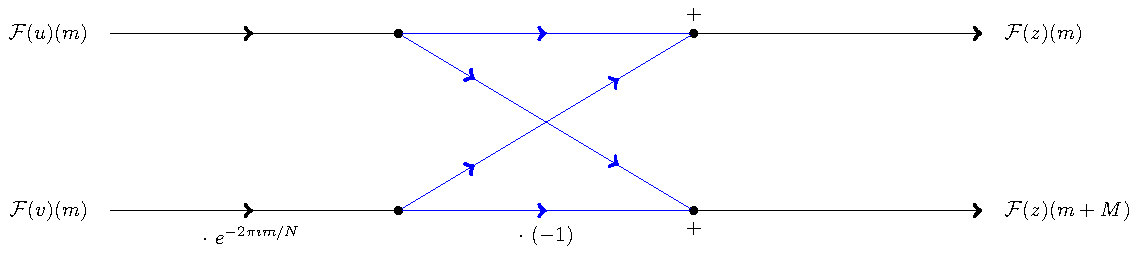
\includegraphics[width=1\textwidth]{./slike-latex/metulj}
\caption{Metulj - osnovni primer izračuna DFT. Pri štetju operacij, ki jih potrebujemo pri programski opremi (hardware), velkokrat štejejo število operacij v enotah metulja.}
\end{figure}
%

Originalni problem izračuna Fourierove transformacije na vektorju dolžine $N$ znamo z nkeja računske manipulacije torej prevesti na podproblema velikosti $N/2$. Za podprobleme sode velikosti bi lahko zgornji postopek ponovili. V primeru, ko je $N$ potenca števila 2, tj.\ $N = 2^n$ za $n \in \N$, bomo lahko problem razdelili vse do podproblemov velikosti 1. Zaradi lažjega zapisa, bomo za število potrebnih kompleksnih množenj pri izračunu DFT na vektorju dolžine $N$, uvedli oznako $E(N)$.
%
\begin{lema}
Naj bo $N = 2^n$ za $n \in \N$. Tedaj velja
\begin{equation*}
  E(N) \leq \frac{1}{2} N \log_2N.
\end{equation*}
\end{lema}
%
\begin{dokaz}
Dokaz naredimo z indukcijo na $n \in \N$. Baza indukcije je v primeru $n = 1$, ko je vektor $z$ dolžine 2, $z = (a, b)$. Z direktno uporabo enodimenzionalne Fourierove transformacije lahko izračunamo $\F(z) = (a + b, a - b)$, za kar ne potrebujemo kompleksnih množenj. Dobimo, da je $E(2) \leq \frac{1}{2} 2 \log_2 2 = 1$, kar pomeni, da v primeru $n = 1$ lema velja. Predpostavimo sedaj, da lema velja za $n - 1$ in dokažimo, da velja za $n$. Iz postopka v dokazu prejšnje leme je razvidno, da je za izračun vektorja $z$ dolžine $N = 2M$ potrebnih največ $2E(M) + M$ kompleksnih množenj. Z uporabo te opazke in indukcijske predpostavke sledi izračun
\begin{equation*}
  E(2^n) \leq 2 E(2^{n-1}) + 2^{n-1} \leq 2\frac{1}{2} 2^{n-1} \log_{2} 2^{n-1} + 2^{n-1} = n 2^{n-1} = \frac{1}{2} n 2^n = \frac{1}{2} N \log_2N,
\end{equation*}
ki pokaže, da lema velja za vsak $n \in \N$.
\end{dokaz}
%
Sedaj pa si oglejmo primer, ko $N$ ni sodo število, ampak gre za sestavljeno število $N = pq$. V tem primeru lahko namreč nekoliko posplošimo zgornjo lemo.
%
\begin{lema}
Naj bosta $p, q \in \N$, $N = pq$ in $z \in \l^2(\Z_N)$. Za $k \in \set{0, 1, \ldots, q-1}$ definiramo zaporedje vektorjev $w_0, w_1, \ldots, w_{p-1} \in \l^2(\Z_q)$ s formulo
$$w_l(k) = z(kp + l).$$
Zaporedje vektorjev $v_0, v_1, \ldots, v_{q-1} \in \l^2(\Z_p)$ definiramo za $l \in \set{0, 1, \ldots, p-1}$ s formulo
$$v_b(l) = e^{-\frac{2\pi\imath bl}{N}} \F(w)(b).$$
Tedaj za $a \in \set{0, 1, \ldots, p-1}$ in $b \in \set{0, 1, \ldots, q-1}$ velja
\begin{equation}\label{eq:aqb}
\F(z)(aq + b) = \F(v_b)(a).
\end{equation}
\end{lema}
%
\begin{dokaz}
%
Osnovni izrek o deljenju naravnih števil nam pove, da lahko vsako število $m \in \set{0, 1, \ldots, N-1}$ zapišemo v obliki $m = aq + b$ za $a \in \set{0, 1, \ldots, p-1}$ in $b \in \set{0, 1, \ldots, q-1}$. Torej znamo po lemi s formulo \eqref{eq:aqb} izračunati $\F(z)(m)$ za vsak $m \in \set{0, 1, \ldots, q-1}$.

Po osnovnem izreku o deljenju lahko zapišemo vsak $n \in \set{0, 1, \ldots, N-1}$ kot $n = kp + l$ za $k \in \set{0, 1, \ldots, p-1}$ in $l \in \set{0, 1, \ldots, q-1}$. Z uporabo tega zapisa števila $n$ in novo definiranimi zaporedji iz predpostavk leme izračunamo:
\begin{align*}
  \F(z)(aq + b) & = \sum_{n=0}^{N-1} z(n) e^{-\frac{2\pi\imath(aq + b)n}{N}} = \sum_{l=0}^{p-1} \sum_{k=0}^{q-1} z(kp + l)e^{-\frac{2\pi\imath(aq + b)(kp + l)}{pq}} \\
  & = \sum_{l=0}^{p-1} e^{-2\pi\imath al}{p} e^{-\frac{2\pi\imath bl}{N}} \sum_{k=0}^{q-1} w_l(k) e^{-\frac{2\pi\imath bk}{q}} = \sum_{l=0}^{p-1} e^{-\frac{2\pi\imath al}{p} e^{-\frac{2\pi\imath bl}{N}}} \F(w_l)(b) \\
  & = \sum_{l=0}^{p-1} e^{-\frac{2\pi\imath al}{p}} v_b(l) = \F(v_b)(a).
\end{align*}
\end{dokaz}
%
Sedaj pa si poglejmo koliko kompleksnih množenj je potrebno v primeru, ko je $N = pq$ sestavljeno število. Ideja je podobna kot v zgornjem dokazu. Najprej moramo izračunati vektorje $\F(w_l)$ za $l \in \set{0, 1, \ldots, p-1}$. Za vsak posamezen $\F(w_l)$ potrebujemo $E(q)$ kompleksnih množenj, skupno torej $p E(q)$. Dobljene vektorje $\F(w_l)(b)$ dolžine $q$ moramo nato pomnožiti z $e^{-\frac{2\pi\imath bl}{N}}$, kar zahteva dodatnih $pq$ kompleksnih množenj. Ko tako dobimo vektorje $v_b(a)$, moramo izračunati $\F(v_b)(a)$ za $b \in \set{0, 1, \ldots, q-1}$, kar zahteva dodatnih $qE(p)$ kompleksnih množenj. Skupno je torej za izračun FFT vektorja dolžine $pq$ potrebnih
\begin{equation}
  E(pq) \leq pE(q) + qE(p) + pq
\end{equation}
kompleksnih množenj. Kaj pa se zgodi v primeru, ko je $N$ praštevilo? Tedaj na vektorju ne moremo uporabiti FFT. Vendar pa še ni vse izgubljeno, vektor lahko namreč na koncu podaljšamo z ničlami do željene velikosti, ki omogoča izvedbo FFT. Zaradi dodanih ničel namreč ne povzročimo velike škode, izračun pa postane opazno hitrejši.

Od tu dalje bomo sedaj predpostavili, da je $N$ potenca števila 2, tj.\ $N = 2^n$. Tedaj lahko $m \in \set{0,1 \ldots N-1}$ zapišemo v obliki polinoma $m = m_0 + m_1 \cdot 2 + m_2 \cdot 2^2 + \ldots + m_{n-1} \cdot 2^{n-1}$, kjer so $m_0, m_1, \ldots, m_{n-1} \in \set{0, 1}$. Za $z \in \l^2(\Z_N)$ bomo pisali $z(m) = z(m_{n-1}, m_n, \ldots, m_1, m_0)$. Za $k = k_0 + k_1 \cdot 2 + k_2 \cdot 2^2 + \ldots + k_{n-1} \cdot 2^{n-1}$, $k_0, k_1, \ldots, k_{n-1} \in \set{0, 1}$ izračunamo
%
\begin{align*}
 & \F(z)(k) = \sum_{m=0}^{N-1} z(m) e^{-\frac{2\pi\imath km}{N}} \\
 & = \sum_{m_0 = 0}^1 \sum_{m_1 = 0}^1 \cdots \sum_{m_{n-1} = 0}^1 z(m_{n-1}, m_{n-2}, \ldots, m_1, m_0) \cdot \\
 & \cdot \exp\left(\frac{-2\pi\imath(k_0 + k_1 2 + k_2 2^2 + \ldots + k_{n-1} 2^{n-1})(m_0 + m_1 2 + m_2 2^2 + \ldots + m_{n-1} 2^{n-1})}{2^n}\right). 
\end{align*}
%
Eksponent razbijemo na produkte glede na vsoto $m_0 + m_1 2 + m_2 2^2 + \ldots + m_{n-1} 2^{n-1}$, poenostavimo dobljeni izraz in ga vstavimo v formulo za $\F(z)(k)$. Dobimo:
%
\begin{align*}
\F & (z)(k) = \sum_{m_0 = 0}^1 \sum_{m_1 = 0}^1 \cdots \sum_{m_{n-1} = 0}^1 z(m_{n-1}, m_{n-2}, \ldots, m_1, m_0) \cdot \exp\left(\frac{-2\pi\imath k_02^{n-1}m_{n-1}}{2^n}\right) \\
& \cdot \exp\left(\frac{-2\pi\imath (k_0 + k_1 2)2^{n-2}m_{n-2}}{2^n}\right) \cdots \exp\left(\frac{-2\pi\imath (k_0 + k_1 2 + \cdots +  k_{n-1} 2^{n-1}) m_0}{2^n}\right).
\end{align*}
%
Notranja vsota je odvisna od spremenljivk $m_0, m_1, \ldots, m_{n-2}$ in $k_0$, nič pa ni odvisna od $k_1, k_2, \ldots, k_{n-1}$. Lahko definiramo
\begin{align*}
  y_1(k_0, m_{n-2}, & m_{n-3},  \ldots, m_0) = \\
  & = \sum_{m_{n-1}=0}^{1} z(m_{n-1},m_{n-2},\ldots,m_1,m_0) \cdot \exp\left(-\frac{2\pi\imath k_0 2^{n-1}m_{n-1}}{2^n}\right)\\
  & = z(0,m_{n-2},\ldots,m_1,m_0) \cdot 1 + z(1,m_{n-2},\ldots,m_1,m_0)\cdot \exp\left(-\frac{2\pi\imath k_0 2^{n-1}}{2^n}\right).
\end{align*}
%
Izračun $y_1$ zahteva le eno kompleksno množenje za vsako izmed $2^n$ možnih vrednosti parametrov $k_0, m_{n-2}, m_{n-1}, \ldots, m_1, m_0$. Za izračun vseh možnih vrednosti izraza $y_1$ potrebujemo torej $2^n$ kompleksnih množenj.

Na naslednjem koraku lahko sedaj izračunamo $y_2$ s formulo
\begin{align*}
  y_2(k_0, k_1, & m_{n-3},  \ldots, m_0) = \\
  & = \sum_{m_{n-1}=0}^{1} y_1(k_0, m_{n-2},\ldots,m_1,m_0) \cdot \exp\left(-\frac{2\pi\imath (k_0 + k_1 2) 2^{n-2}m_{n-2}}{2^n}\right).
\end{align*}
%
Ta izračun prav tako potrebuje $2^n$ kompleksnih množenj. Naprej nadaljujemo podobno. Poglejmo si shemo, ki prikazuje kako izračunamo $z$:
%
\begin{align*}
 z(m_{n-1}, m_{n-2}, \ldots, m_1, m_0) & \to y_1(k_0, m_{n-2}, \ldots, m_1, m_0) \\
 y_1(k_0, m_{n-2}, m_{n-3},\ldots, m_0) & \to y_2(k_0, k_1, m_{n-3}, \ldots, m_0) \\
 & \vdots \\
 y_{n-1}(k_0, k_1, k_2, \ldots, k_{n-2}, m_0) & \to y_n(k_0, k_1, k_2, \ldots, k_{n-2}, k_{n-1}) \;.
\end{align*}
%
Kot smo rekli, na vsakem koraku potrebujemo $2^n$ kompleksnih množenj, imamo $n$ korakov, skupno torej $n\cdot 2^n = N \log_2N$ kompleksnih množenj. Poleg tega opazimo tudi, da po izračunu $y_{j}$ vektorja $y_{j-1}$ ne potrebujemo več. Izračune vektorjev lahko torej delamo na mestu, kar pomeni, da lahko na vsakem koraku prejšnje podatke zamenjamo z novimi trenutnimi podatki.

Prav tako lahko z $\frac{N}{2} \log_2N$ kompleksnimi množenji izračunamo IDFT po formuli $\F^{-1}(w)(n) = \frac{1}{N} \F(w)(N-n)$.

S pomočjo DFT in IDFT lahko sedaj pospešimo tudi računanje konvolucije. Vemo namreč, da velja
$$z \ast w = \F^{-1}(\F(z)\F(w)).$$
Skupno porabimo za izračun konvolucije $N + \frac{3N}{2}\log_2N$ kompleksnih množenj.
%
\subsubsection{Dvodimenzionalna hitra diskretna Fourierova transformacija}
V trditvi~\ref{trd:2dft} smo definirali $y(n_1, m_2)$. Direkten izračun vseh vrednosti $y(n_1, m_2)$ zahteva $N_1 N_2^2$ kompleksnih množenj, za tem pa direkten izračun vseh vrednosti za $\F(z)(m_1, m_2)$ zahteva $N_1^2 N_2$ kompleksnih množenj. Skupaj torej potrebujemo $N_1 N_2 (N_1 + N_2)$ množenj.
%
\begin{trditev}
Naj bosta $N_1$ in $N_2$ števili potence 2. Z uporabo računanja od zgoraj namesto direktnega računanja, se da $\F(z)$ izračunati z uporabo največ $\frac{1}{2} N_1 N_2 \log_2(N_1 N_2)$ kompleksnih množenj.  
\end{trditev}
%
%%
%% Signal
\section{Transformacije slik}\label{sec:TransformacijeSlik}
%
%TODO Poveš kako bo predstavljena naša slika.
\subsection{Signali}\label{sec:Signali}
%
\emph{Signali} so funkcije ene ali več spremenljivk, ki nam posredujejo določene informacije o nekem fizikalnem pojavu, npr.\ podatke o zvočni frekvenci glasbila. Podatke, ki bi jih želeli dobiti iz vhodnega signala, največkrat ne dobimo direktno, temveč moramo vhodni signal pred njegovo analizo pretvoriti v nek drug sistem oz.\ zapis. Matematično povedano, na funkciji (matematični predstavitvi signala) moramo izvesti neko transformacijo. Predstavitev signala s funkcijo in transformacije, ki jih izvedemo na tej funkciji, so odvisne od lastnosti, ki jim preučevani signal ustreza (periodičnost, končnost, zveznost \ldots).
%
% TODO iz [0, 255], ker je digitalna slika
Slika je signal, ki ga uvrščamo v skupini diskretnih in digitalnih signalov. Če imamo sivinsko sliko, potem je osnovna predstavitev signala $n \times m$ matrika, ki ima vrednosti elementov z intervala $[0, 1]$. Pri tem sta $n$ višina in $m$ širina slike, vrednosti elementov pa nastavimo na vrednosti pripadajočih slikovnih točk. Sliko bomo označili z $I$, njene slikovne točke pa z $I(x, y)$.

\emph{Transformacijo slike} $I$ bomo označili s $T$ in jo definirali kot:
%
$$T: I(x, y) \to J(u, v).$$
%
Obravnavali bomo tri skupine transformacij:
%
\begin{enumerate}
\item točkovne transformacije (izhodna vrednost transformacije je odvisna le od ene vrednosti; ni nujno, da uporabimo pri izračunu vrednosti; 
\item lokalne transformacije (izhodna vrednost transformacije $T$ je odvisna od vseh vrednosti v soseski pripadajoče slikovne točke vhodne slike);
\item globalne transformacije (izhodna vrednost transformacije $T$ v točki $(x, y)$ je odvisna od vseh vrednosti vhodne slike).
\end{enumerate}
%
V nadaljevanju bomo spoznali posamezne skupine teh transformacij in njihovo praktično vrednost.
%
\subsection{Točkovne transformacije}
%
Točkovne transformacije pri izračunu vrednosti $T(x, y)$ uporabijo le podatek o vrednosti slikovne točke $(x, y)$ (glej sliko \ref{fig:tockovnaT}). Za izračun točkovne transformacije $T$ na $n \times m$ veliki sliki $I$ porabimo $\O(k\cdot nm)$ časa, pri čemer je $O(k)$ časovna zahtevnost izračuna vrednosti $T(x, y)$ za eno slikovno točko. Ker za izračun potrebujemo le vrednost dotične slikovne točke, lahko izvedemo računanje na mestu, torej pri računanju ne potrebujemo dodatnega pomnilnika.

%
\begin{figure}[htbp]
  \centering
  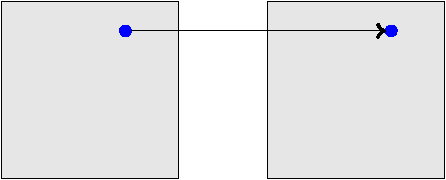
\includegraphics[width=0.6\textwidth]{./slike-latex/tockovnaT}
  \caption{Točkovna transformacija vhodne slike.}
  \label{fig:tockovnaT}
\end{figure}
%

Enostavni primeri točkovnih transformacij so: rotacija slike, zrcaljenje, skrčitev, \ldots % TODO une weird k swirl itd. dodaj
Za nas pomembne točkovne transformacije so tiste, ki spreminjajo barve itd. %TODO lepo napiši to
%% Lokalne transformacije
\subsection{Lokalne transformacije}\label{sec:LokalneTransformacije}
%
Pri lokalnih transformacijah za izračun $T(x, y)$ v slikovni točki $(x, y)$ uporabimo vrednosti slikovnih točk v njeni soseki (glej sliko \ref{fig:lokalnaT}).

%
\begin{figure}[htbp]
  \centering
  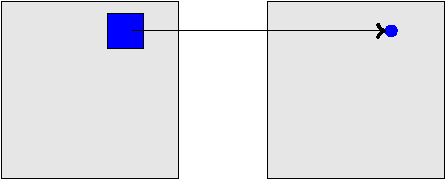
\includegraphics[width=0.6\textwidth]{./slike-latex/lokalnaT}
  \caption{Lokalna transformacija na sliki.}
  \label{fig:lokalnaT}
\end{figure}
%

Na področju obdelave slik so tovrstne transformacije uveljavljen postopek, ki mu pravimo \emph{filtriranje}. V tem kontekstu je $T(x, y)$ utežena vsota vrednosti slikovnih točk iz pravokotne okolice slikovne točke $(x, y)$. Uteži shranimo v \emph{filtrirno masko} $h$, ki je $(2b + 1)\times(2a + 1)$ matrika z realnimi vrednostmi. Običajno so filtrirne maske kvadratne in manjših velikosti. Vrednosti $T(x, y)$, ki jih dobimo pri filtriranju slike $I$ s filtrom $h$, izračunamo s pomočjo konvolucije:
%
\begin{equation}\label{eq:filtriranje}
T(x, y) = \frac{(I \ast h)(x,y)}{\sum_{s=-a}^{a} \sum_{t=-b}^{b} h(s, t)} = \frac{\sum_{s=-a}^{a} \sum_{t=-b}^{b} h(s, t) I(x-s, y-t)}{\sum_{s=-a}^{a} \sum_{t=-b}^{b} h(s, t)} \;.
\end{equation}
%
\begin{opomba}
V literaturi velikokrat poudarijo, da gre za filtriranje v slikovni domeni, saj poznamo tudi filtriranje v Fourierovi domeni, ki pa ga bomo mi spoznali malce kasneje.
\end{opomba}
%
\begin{opomba}
Kot vidimo v enačbi \eqref{eq:filtriranje}, smo rezultat, ki ga dobimo pri konvoluciji slike in filtrirne maske, normirali. Namesto tega bi lahko za filtrirno masko zahtevali, da je normirana (tj.\ ima vsoto vrednosti 1). Filtrirne maske, ki jih bomo predstavili v našem delu, bomo zapisali v normirani obliki. 
\end{opomba}
%
Postopek filtriranja obsega večji del področja pri obdelavi slik. Z uporabo filtrirnih mask lahko poiščemo, zgladimo ali izostrimo robove na sliki, zameglimo celotno sliko \ldots V nadaljevanju bomo predstavili primere filtrirnih mask, ki jih bomo kasneje tudi uporabljali v algoritmih za likovno upodabljanje slik.
%%% Tehnični pogled na filtriranje
\subsubsection{Tehnični pogled na filtriranje}\label{sec:TehnicniPogledNaFiltriranje}
%
Za boljšo predstavo bomo sedaj filtriranje predstavili še grafično. Filtrirno masko $h$ (glej \ref{fig:maskah}) najprej rotiramo za $180 \degree$, da dobimo filtrrino masko $h'$. Slednjo nato postavimo na vhodno sliko $I$ tako, da center maske sovpada s slikovno točko na sliki $I$, v kateri želimo izračunati vrednost $T(x, y)$. Vrednost $T(x, y)$ sedaj izračunamo tako, da pomnožimo istoležne vrednosti v matriki $h'$ in na sliki $I$ (glej sliko \ref{fig:pomnoziI}). Za razliko od točkovne transformacije, pri kateri smo novo vrednost lahko kar shranili na mesto $(x, y)$ v matriki $I$, moramo naračunane vrednosti shraniti v novo matriko $J$.

V primeru, ko želimo izračunati npr.\ vrednost $T(x, y)$ za slikovno točko v kotu slike, del filtrirne maske ne pokriva slike $I$. Da se izognemu temu problemu, sliko $I$, pred filtriranjem s filtrirno masko velikosti $(2a + 1) \times (2a + 1)$, obrobimo naokoli z $a$ celicami. Njihove vrednosti lahko nastavimo na več načinov (za primer glej sliko \ref{fig:obrobaI}). Pri tem opazimo, da lahko sedaj (ob privzetku, da filtrirane vrednosti računamo po vrsti) namesto, da za novo naračunane vrednosti ustvarimo novo matriko $J$, pri računanju vrednosti $T(x, y)$ novo vrednost shranimo na mesto $(x-a, y-1)$, saj te vrednosti ne bomo več potrebovali pri izračunu ostalih vrednosti. S tem v primeru velikih slik naredimo velik prihranek pri pomnilniku.
%
\begin{primer}
%TODO Zakaj ne poravna slikic ????

\begin{figure}[htbp]
  \centering
  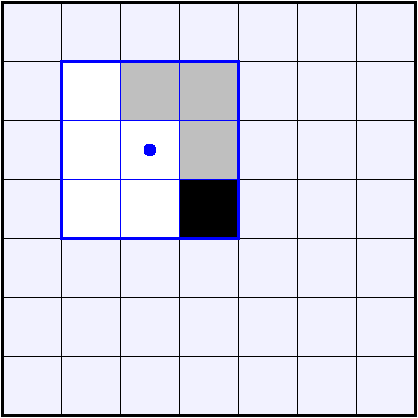
\includegraphics[width=0.2\textwidth]{./slike-latex/filter1}\ \ \ \ \ \ 
  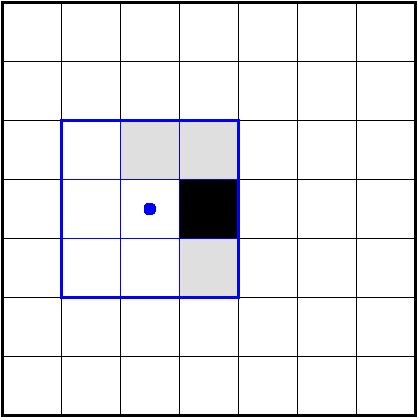
\includegraphics[width=0.2\textwidth]{./slike-latex/filter2}\ \ \ \ \ \ 
  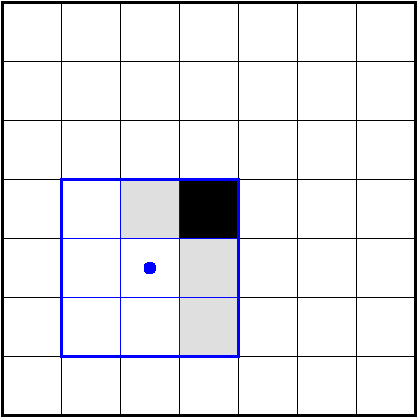
\includegraphics[width=0.2\textwidth]{./slike-latex/filter3}\ \ \ \ \ \ 
  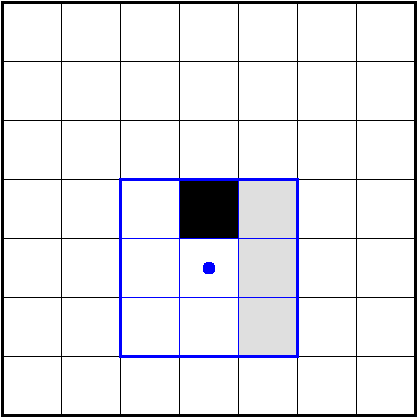
\includegraphics[width=0.2\textwidth]{./slike-latex/filter4}\\[0.6cm]

  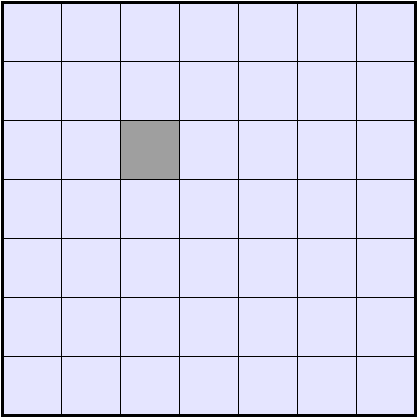
\includegraphics[width=0.2\textwidth]{./slike-latex/filter1s}\ \ \ \ \ \ 
  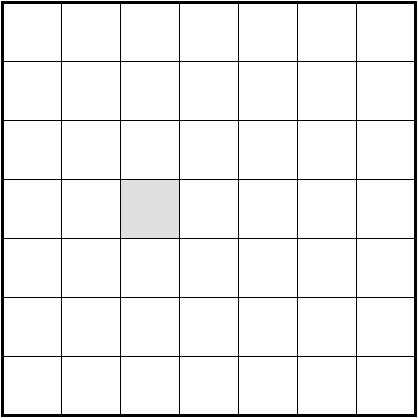
\includegraphics[width=0.2\textwidth]{./slike-latex/filter2s}\ \ \ \ \ \ 
  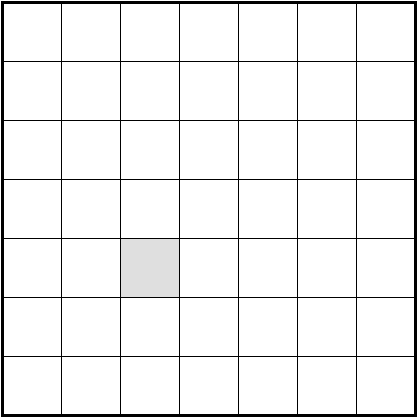
\includegraphics[width=0.2\textwidth]{./slike-latex/filter3s}\ \ \ \ \ \ 
  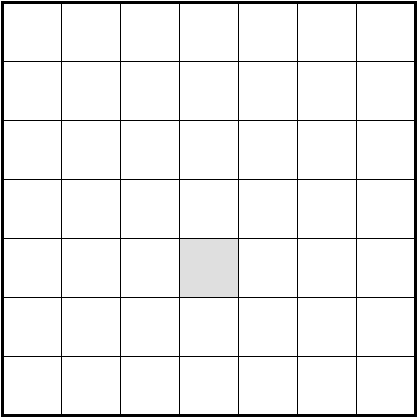
\includegraphics[width=0.2\textwidth]{./slike-latex/filter4s}
  \caption{Filtriranje v slikovni domeni.}
  \label{fig:filtriranje}
\end{figure}

\end{primer}
%
Omenimo naj še, da so filtrirne maske, za razliko od maske v zgornjem primeru, običajno simetrične. Pri računanju filtriranih vrednosti lahko zato preskočimo rotacijo filtrirne maske, saj dobimo nazaj isto filtrirno masko.

Zgoraj predstavljeni postopek je osnovni način filtriranja. V naslednjem podrazdelku, kjer bomo izpeljali filter za zameglitev slike, pa bomo spoznali še drug pristop k filtriranju.
%
\subsubsection{Zamegljenje slike}\label{sec:ZamegljenjeSlike}
%
\emph{Impulzna slika} $\Delta_{p,q}$ je slika, ki ima vrednosti vseh slikovnih točk, razen ene z vrednostjo 1, enake 0. Definirana je kot:
$$
\Delta_{p,q}(x - p, y - q)=
\begin{cases}
  1 & \mbox{če } (x, y) = (p,q), \\ 
  0 & \mbox{sicer}.
\end{cases}
$$
%
Konvolucijo slike $I$ z $w$ uteženo impulzno sliko $\Delta_{p,q}$ izračunamo kot:
\begin{equation*}
[I \ast w\Delta_{p,q}](x,y) = w \cdot I(x - p, y - q) \;.
\end{equation*}
%
Postopek za izračun filtrirane slike:
%
\begin{enumerate}
  \item Za vsako celico filtrirne maske $h$ naredimo eno prazno matriko velikosti $(h+2a)\times(w+2a)$.
  \item V vsako izmed teh praznih matrik kopiramo vhodno sliko $I$ tako, da
\end{enumerate}
%
Na sliki \ref{fig:premakniSlike}
%
\begin{primer}
%TODO Zakaj ne poravna slikic ????

\begin{figure}[htbp]
  \centering
  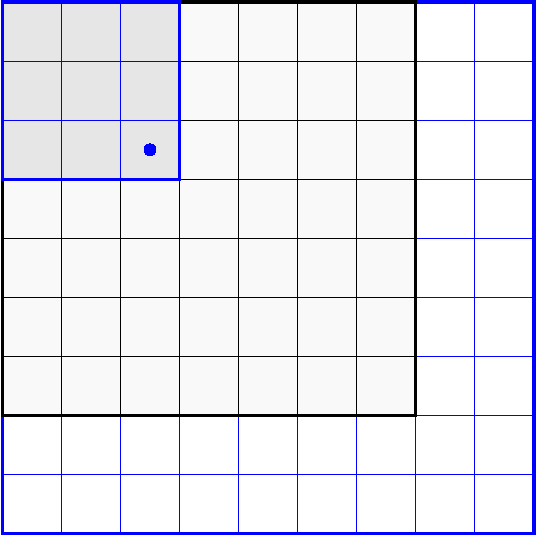
\includegraphics[width=0.2\textwidth]{./slike-latex/filterMSI1}\ \ \ \ \ \ 
  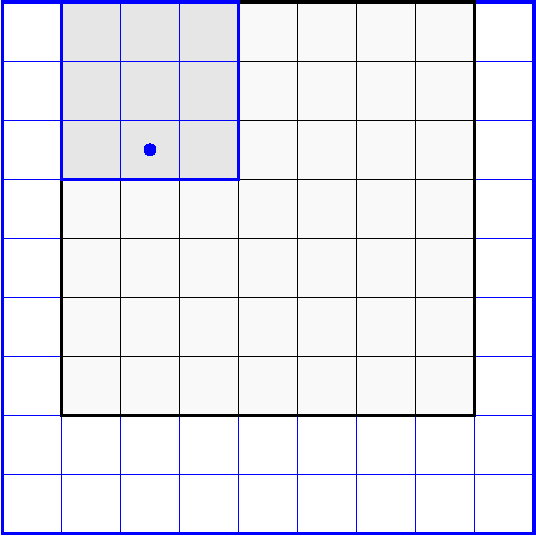
\includegraphics[width=0.2\textwidth]{./slike-latex/filterMSI2}\ \ \ \ \ \ 
  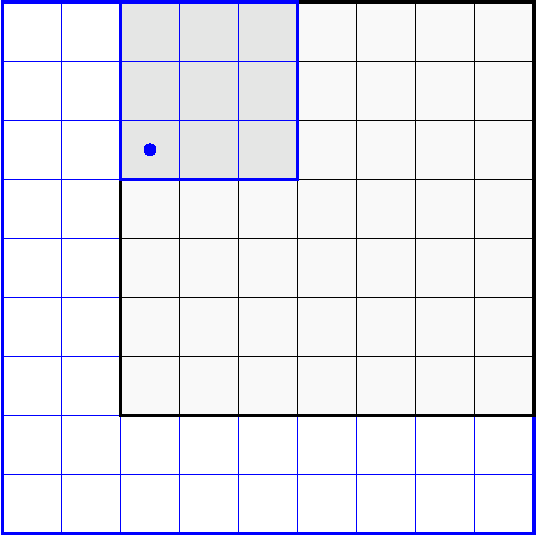
\includegraphics[width=0.2\textwidth]{./slike-latex/filterMSI3}\\[0.6cm]
  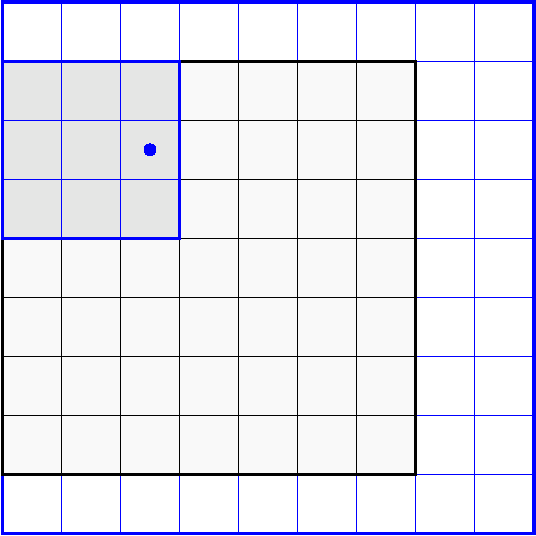
\includegraphics[width=0.2\textwidth]{./slike-latex/filterMSI4}\ \ \ \ \ \ 
  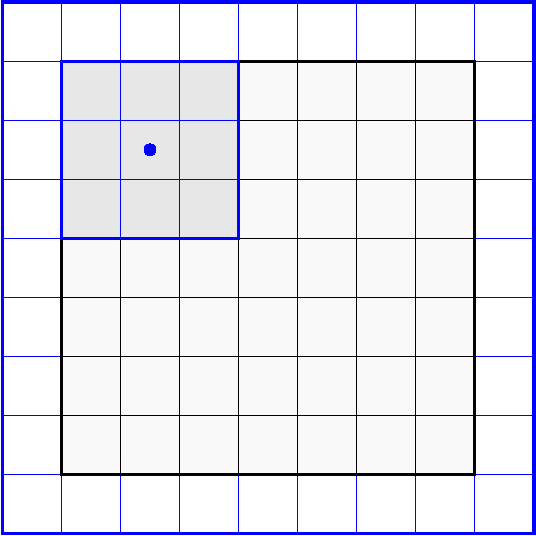
\includegraphics[width=0.2\textwidth]{./slike-latex/filterMSI5}\ \ \ \ \ \ 
  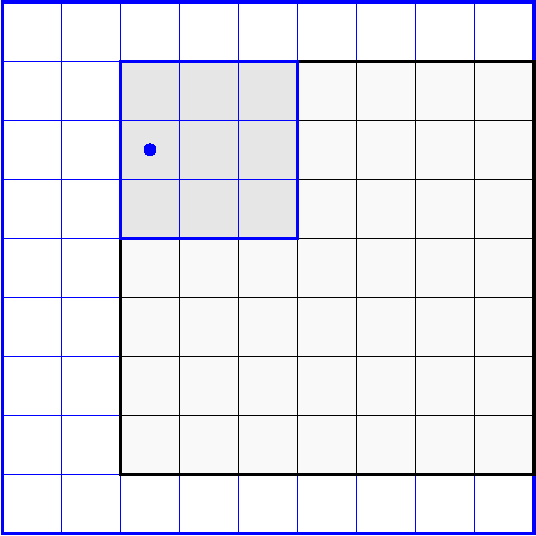
\includegraphics[width=0.2\textwidth]{./slike-latex/filterMSI6}\\[0.6cm]
  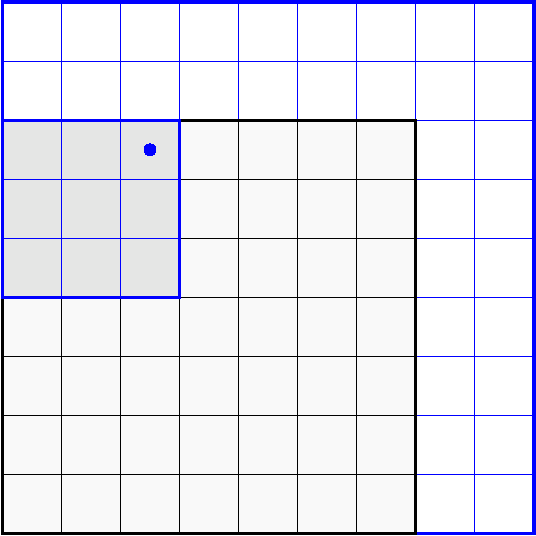
\includegraphics[width=0.2\textwidth]{./slike-latex/filterMSI7}\ \ \ \ \ \ 
  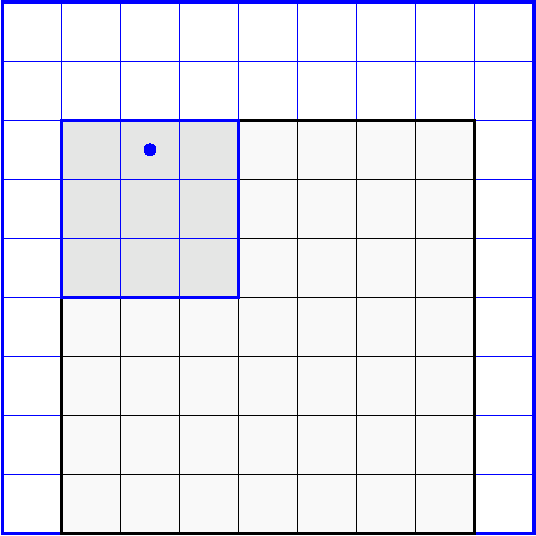
\includegraphics[width=0.2\textwidth]{./slike-latex/filterMSI8}\ \ \ \ \ \ 
  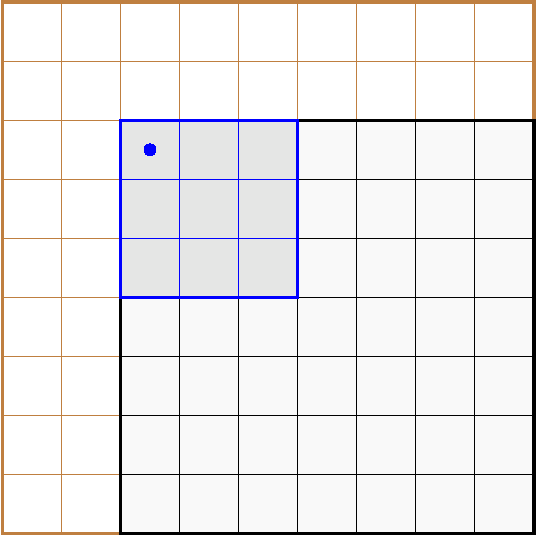
\includegraphics[width=0.2\textwidth]{./slike-latex/filterMSI9}
  \caption{Filtriranje v slikovni domeni.}
  \label{fig:filtriranje}
\end{figure}

\end{primer}
%
\subsubsection{Filter za zaznavo robov na sliki}
Kaj je rob ?

%
\begin{figure}[htbp]
  \centering
  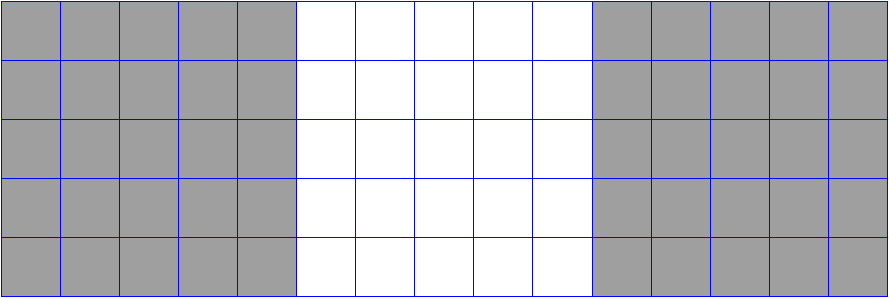
\includegraphics[width=0.45\textwidth]{./slike-latex/rob-slika}\ \ \ 
  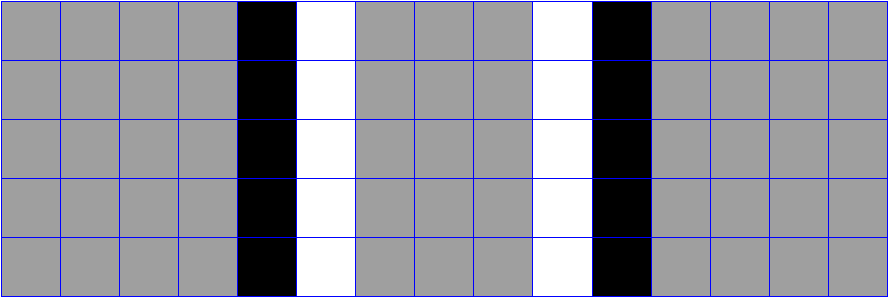
\includegraphics[width=0.45\textwidth]{./slike-latex/rob-center}\\[0.5cm]
  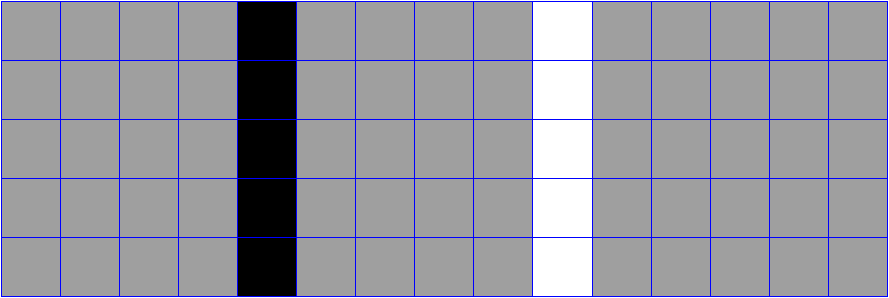
\includegraphics[width=0.45\textwidth]{./slike-latex/rob-naprej}\ \ \ 
  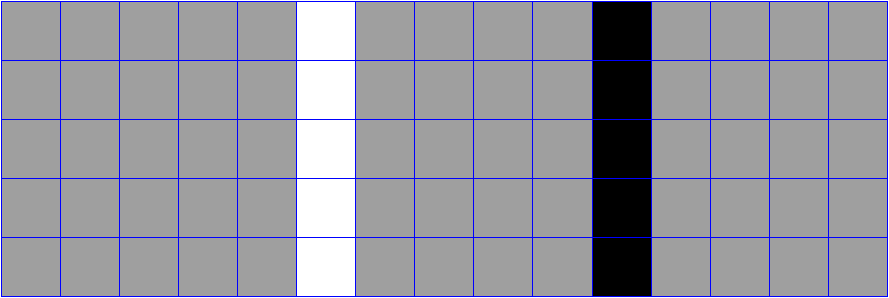
\includegraphics[width=0.45\textwidth]{./slike-latex/rob-nazaj}
  \caption{Robovi.}
  \label{fig:robovi}
\end{figure}
%

Ne maram ljudi.

%
\begin{figure}[htbp]
  \centering
  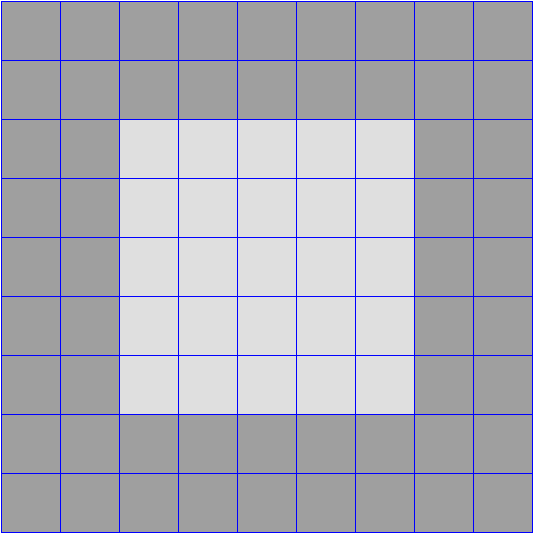
\includegraphics[width=0.23\textwidth]{./slike-latex/rob-kvadrat}\ \ \ 
  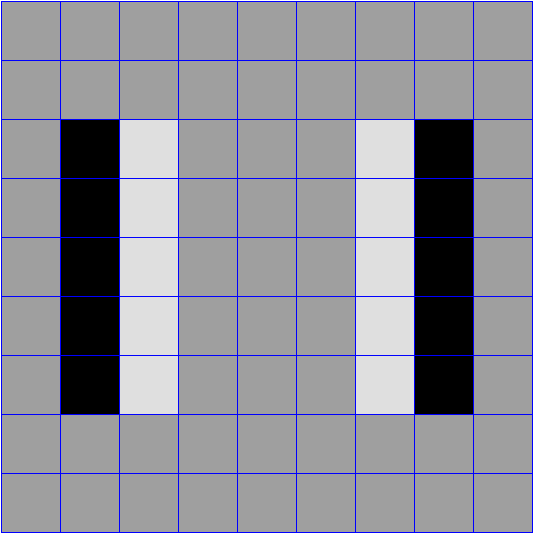
\includegraphics[width=0.23\textwidth]{./slike-latex/rob-kvadrat-vodoravno}\ \ \  
  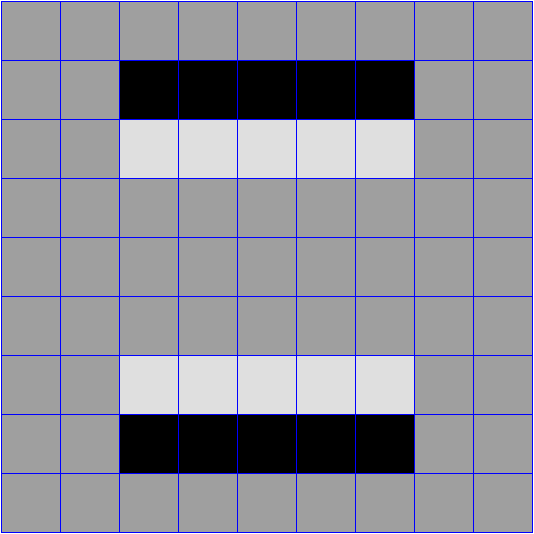
\includegraphics[width=0.23\textwidth]{./slike-latex/rob-kvadrat-navpicno}\ \ \ 
  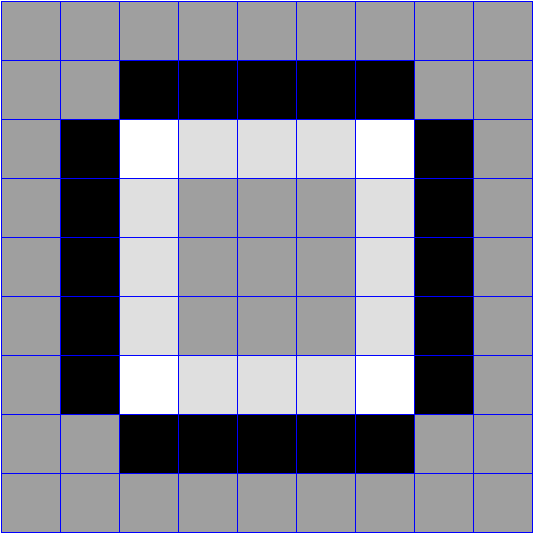
\includegraphics[width=0.23\textwidth]{./slike-latex/rob-kvadrat-vod-nav}
  \caption{Robovi v kvadratu.}
  \label{fig:roboviKvadrat}
\end{figure}
%
\subsection{Globalne transformacije}
Pri globalnih transformacijah za izračun vrednosti $T(x, y)$ upoštevamo vrednosti vseh slikovnih točk na sliki (glej sliko \ref{fig:globalnaT}). Najbolj pomembna transformacija te vrste je za nas Fourierova transformacija. V tem podrazdelku si bomo pogledali kakšna je praktična vrednost Fourierove transformacije pri obdelavi slik. 

%
\begin{figure}[htbp]
  \centering
  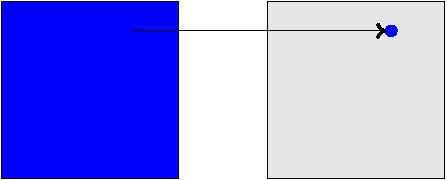
\includegraphics[width=0.6\textwidth]{./slike-latex/globalnaT}
  \caption{Globalna transformacija.}
  \label{fig:globalnaT}
\end{figure}
%

Kot smo videli v prvem razdelku tega poglavja lahko sliko $I$, namesto v običajni evklidski bazi, zapišemo v Fourierovi bazi:
%
\begin{equation*}
I(x, y) = \sum_{v = 0}^{N_1 - 1} \sum_{u = 0}^{N_2 - 1} \F(I)(u, v) F_{u, v}(x, y)\;.
\end{equation*}
%
Za vizualno predstavitev slike bomo na Fourierovo transformacijo pogledali z nekoliko bolj fizikalnega vidika. Za začetek si poglejmo dvodimenzionalne sinusoide.
%
\subsubsection{Dvodimenzionalne sinusoide}
 Zaradi poenostavitve zapisa naj velja $N_1 = N_2 = N$. Tedaj bomo zapisali $F_{u,v}(x,y)$ v polarni obliki:
%
$$F_{u, v}(x, y) = e^{\pm \imath \frac{2\pi \omega}{N}\cdot (u \sin \theta + v \cos \theta)},$$
%
kjer je $y = \omega \sin \theta$, $x = \omega \cos \theta$ in $\omega = \sqrt{x^2 + y^2}$.
%
Če pišemo še $\lambda = \frac{N}{\omega}$, dobimo
$$F_{u, v}(x, y) = \cos[\frac{2\pi}{\lambda} (u \sin \theta + v \cos \theta)] \pm \imath \sin[\frac{2\pi}{\lambda}(u \sin \theta + v \cos \theta)].$$
%
Tako realni del $F_{u, v}(x, y)$
$$\cos[\frac{2\pi}{\lambda} (u \sin \theta + v \cos \theta)]$$
kot imaginarni del
$$\pm \sin\left[\frac{2\pi}{\lambda}(u \sin \theta + v \cos \theta)\right]$$
sta sinusoidi z amplitudo $1$, periodo $\lambda$ in smerjo $\theta$.
%
Tedaj je $\frac{2\pi \omega}{N}$ radialna frekvenca, $\frac{\omega}{N}$ je frekvenca in $\lambda = \frac{N}{\omega}$ je dolžina vala sinusoide, merjena v slikovnih točkah.

Dvodimenzionalno sinusoido bomo zapisali s formulo
$$\frac{A}{2} \cdot \left(\cos\left[\frac{2\pi}{\lambda} \cdot (u \cdot \sin \Phi + v \cdot \cos \Phi) + \phi\right] + 1\right),$$
kjer je $A$ amplituda sinusoide in $\phi$ je fazni zamik.
%
\begin{definicija}
Naj bosta $Re$ in $Im$ realni in kompleksni del vrednosti $\F(I)(u, v)$. Definiramo pojme: 
%
\begin{enumerate}
\item \emph{Fourierov spekter}:
$$\abs{\F(I)(u, v)} = \sqrt{Re^2(u, v) + Im^2(u, v)};$$
\item \emph{fazni zamik}:
$$\varPhi(u, v) = \arctan\frac{Im(u, v)}{Re(u, v)};$$
\item \emph{močnostni spekter}:
$$P(u, v) = Re^2(u, v) + Im^2(u, v).$$
\end{enumerate}
\end{definicija}
%
Fourierovo transformacijo lahko z novo definiranimi pojmi zapišemo v polarni obliki:
$$\F(z)(u, v) = \abs{\F(z)(u, v)} e^{-\imath \cdot \varPhi(u, v)}.$$
%
Poveš, da če je pikica v frekvenčni domeni je to sinus v navadni evklidski ravnini.
%
\begin{primer}
Primer slike in njenega Fouirerovega spektra. In primer ene slike, ki bo neka vsota, nekaj nekaj baznih elemntov.
\end{primer}
%
\begin{primer}
Poglejmo si primer, ko imamo isti spekter in različni fazni zamik; ter isti fazni zamik, a različni spekter. Fazni zamik spreminjamo tako, da množimo z matriko $R$. Dobimo razne slike, ena izmed je lepa, ostale so kar nekaj ...		
\end{primer}
%
O spektru in faznem zamiku bomo govorili v nadaljevanju, saj sta to informaciji, ki nam povesta ogromno o sliki. Sedaj pa si najprej poglejmo še o translacijah in rotacijah Fourierove transformacije \ldots

%
\begin{figure}[htbp]
  \centering
  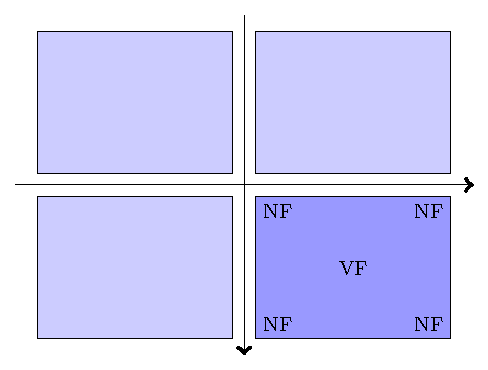
\includegraphics[width=0.49\textwidth]{./slike-latex/DFToriginal}
  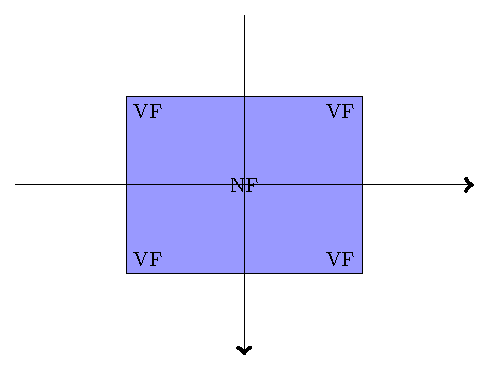
\includegraphics[width=0.49\textwidth]{./slike-latex/DFTpremaknjena}
  \caption{Originalna DFT.}
  \label{fig:DFToriginal}
\end{figure}
%
%%
\section{Barvni modeli}
Poznamo različne barvne modele:
%
\begin{itemize}
\item RGB barvni model;
\item CMY barvni model;
\item HSV barvni model;
\item HSL barvni model;
\item YUV barvni model.
\end{itemize}
%
\subsection{RGB in CMY barvna modela}
RGB barvni prostor predstavimo z enotsko kocko. Oglišča kocke so enaka:

\begin{figure}[htbp]
  \centering
  \subfigure[]{
  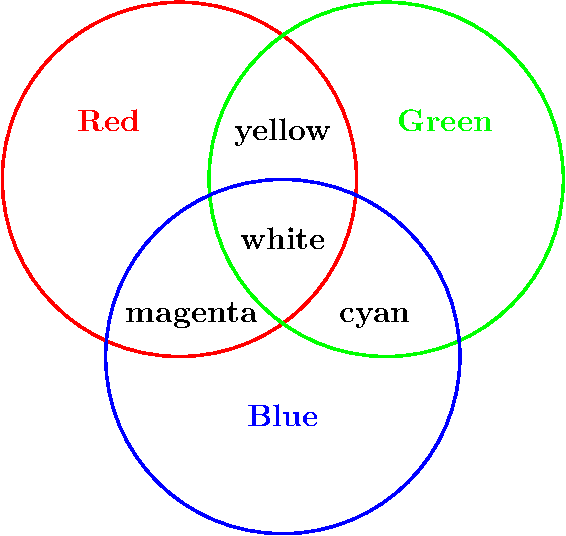
\includegraphics[width=0.31\textwidth]{./slike-latex/RGB}}
  \subfigure[]{
  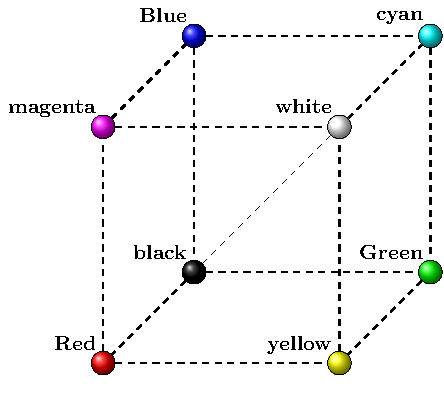
\includegraphics[width=0.31\textwidth]{./slike-latex/kockaRGB}}
  \subfigure[]{
  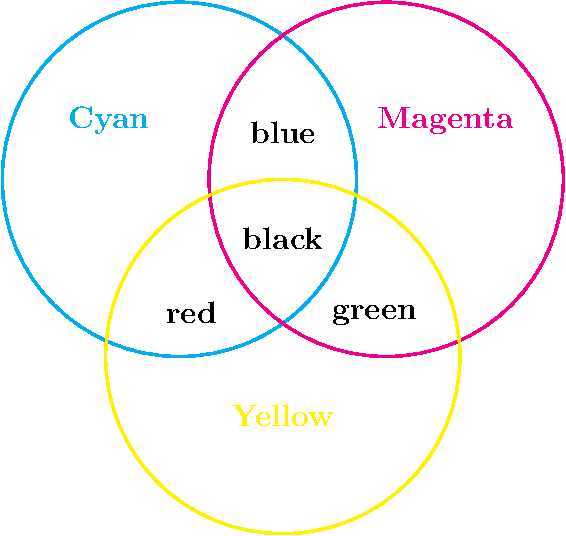
\includegraphics[width=0.31\textwidth]{./slike-latex/CMY}}
  \caption{RGB kocka.}
  \label{fig:rgbcube}
\end{figure}

%
\subsection{HSV in HSL barvna modela}
%
To je pa polarna predstavitev RGB barvnega modela.
%
\subsection{Kubelka--Monk barvni model}
%%
% Odstranjevanje šuma s slike.
\section{Odstranjevanje šuma na sliki}
%
Odstranjevanje (digitalnega) šuma predstavlja pomembno področje pri obdelavi slik, saj ta običajno povzroča motnje in nepravilnosti pri delovanju algoritmov, ki jih uporabljamo za obdelavo slik. Pri tem naj opozorimo, da s pojmom šum mnogi poimenujejo tudi fine strukture in teksture, ki so prisotne na sliki. Slednje namreč tudi predstavljajo težave, vendar pa se moramo njim izogniti pri samem algoritmu za obdelavo slik.

V tem razdelku bomo predstavili merilo uspešnosti za odpravljanje digitalnega šuma na sliki, ki je predstavljen v članku \cite{Buades:NLA}. Nadalje bomo primerjali različne metode, ki so predstavljene v tem članku, in nato metodo nelokalnega odstranjevanja šuma dopolnili z njeno pohitritvijo, opisano v članku \cite{Wang:fastNMD}. V zadnjem delu bomo nato predstavili še implementacije posameznih metod in primerjali eksperimentalno dobljene podatke o učinkovitosti posameznih metod.
%
\subsection{Metoda šuma}
Naj bo $I$ vhodna slika, na kateri je prisoten šum. Zaradi poenostavitve sintakse bomo slikovne točke, namesto z $(x, y)$, označili z $i = (x_i, y_i)$. Vrednosti slikovnih točk na sliki $I$ bomo označili z $v(i)$. Slednjo vrednost lahko zapišemo kot vsoto $v(i) = u(i) + n(i)$, pri čemer $u(i)$ predstavlja vrednost slikovne točke na sliki brez prisotnega šuma in $n(i)$ predstavlja vrednost prisotnega šuma. Z $v$ bomo označili množico vrednosti $v = \set{v(i) \mid i \in I}$, ki jo poimenujemo \emph{realna slika}. \emph{Originalna slika} je množica vrednosti $u = \set{u(i) \mid i \in I}$. Množica $n = \set{n(i) \mid i \in I}$ pa je pristoni \emph{šum} na sliki. Za modeliranje prisotnosti digitalnega šuma na sliki je najboljša izbira \emph{Gaussov beli šum}, tj.\ Gaussove vrednosti s srednjo vrednostjo 0 in standardnim odklonom $\sigma^2$.
%
\begin{definicija}
\emph{Operator šuma} $D_h$ je tak operator, za katerega lahko naredimo dekompozicijo realne slike $v$:
$$v = D_h v + n(D_h, v),$$
kjer je parameter $h$ odvisen od standardnega odklona šuma.
\end{definicija}
%
Od operatorja šuma pričakujemo, da bo množica (slika) $D_h v$ gladkejša od originalne slike. Za dobljeni šum $n(D_h v)$ pa želimo, da čimbolje aproksimira beli šum. Nočemo pa, da bi poleg digitalnega šuma na sliki operator šuma odstranil tudi morebitno prisotno teksturo in pokvaril videz drobnih detajlov na sliki. Ker večina metod deluje na principu povprečenja sosednjih vrednosti slikovnih točk, pa zgornje zahteve povečini pri metodah ne držijo v celoti. Za merilo uspešnosti posameznih metod oz.\ operatorja šuma bomo uvedli t.~i.\ \emph{metodo šuma}.
%
\begin{definicija}
Naj bo $u$ originalna slika in $D_h$ operator šuma, ki je odvisen od parametra $h$. \emph{Metoda šuma} je definirana kot razlika
$$u - D_h u.$$
\end{definicija}
%
Metoda šuma torej predstavlja razliko med originalno sliko $u$ (na kateri ni nujno prisoten šum) in $D_h u$ (originalna slika, na kateri smo uporabili operator šuma). V primeru, ko bi originalna slika vsebovala neko teksturo, vzorce ali določeno strukturo, se te v metodi šuma ne smejo pojaviti, saj bi to kazalo na to, da smo pokvarili videz originalne slike. Metoda šuma mora izgledati kot aproksimacija šuma, celo v primerih, ko je na originalni sliki šum prisoten v zelo majhnih količinah.
%%
\subsection{Lokalni algoritmi za odstranjevanje šuma na sliki}
Predstavili bomo tri metode za odstranjevanje šuma, ki pri računanju operatorja šuma izkoriščajo le lokalne podatke.
% 
% TODO kaj naredim, ker imam x pa y, rečem pa da imam slikovne točke i
\subsubsection{Gaussovo filtriranje}
Gaussovo filtriranje sodi v skupino izotropnega linearnega filtriranja slik, kjer naredimo konvolucijo slike z linearnim simetričnim filtrom. Gaussov filter definiramo s funkcijo
$$G_h(x) \coloneqq \frac{1}{4 \pi h^2} e^{- \frac{\abs{x}^2}{4 h^2}} \;.$$
V tem primeru ima $G_h$ standardni odklon $h$ in velja naslednji izrek.
%
\begin{izrek}
Metoda šuma za Gaussovo filtriranje je za dovolj majhen $h$ enaka
$$u - G_h \ast u = - h^2 \Delta u + o(h^2)\;.$$
\end{izrek}
%
Zgornji izrek dokažemo s pomočjo toplotne enačbe, saj izkoristimo dejstvo, da je fundamentalna rešitev toplotne enačbe porazdeljena po Gaussu (dokaz lahko bralec poišče v \cite{Lind:Gauss-dokaz}).

Izrek nam pove, da bo v harmoničnih delih slike metoda šuma enaka 0, medtem ko bo v bližini linij, robov in delov teksture imela visoke vrednosti. Na zveznih območjih slike bo metoda šuma torej optimalna, saj bo v celoti odstranila prisotni šum in pri tem ohranila videz slike. Deli slike v okolici linij, robov in prisotne teksture na sliki bodo po odstranitvi šuma postali zamegljeni in s tem pokvarili videz slike.
%%
\subsubsection{Anizotropno filtriranje}
Ideje za to vrsto filtriranja so bile predstavljene v \cite{Perona-Malik}. Pri anizotropnem filtriranju (kratica AF) poskušamo dejstvo, da pri Gaussovem filtriranju dobimo zamegljene dele slike, popraviti s tem, da v slikovni točki $i$ naredimo konvolucijo s filtrom $G_h$ le v smeri, ki je ortogonalna na $G(i)$. Pri tem je $G = \sqrt{(\partial_x u)^2 + (\partial_y u)^2}$, $\partial_x u$ in $\partial_y u$ sta gradientni sliki v $x$ in $y$ smeri. Konvolucijo naredimo torej le v ``smeri linije, ki poteka skozi slikovno točko~$i$.''

Operator šuma za AF je za $x$, $G(x) \neq 0$, definiran s funkcijo
%
$$AF_h u(x) = \int G_h(t)\cdot u\left( x + t \frac{G(x)^\perp}{\abs{G(x)}}\right) dt\;.$$
%
Ob predpostavki, da je originalna slika $u$ dvakrat zvezno odvedljiva v $x$, lahko s pomočjo Taylorjeve vrste drugega reda pokažemo veljavnost naslednjega izreka (dokaz bomo tukaj izpustili).
%
\begin{izrek}
Metoda šuma za anizotropni filter $AF$ je na območjih, kjer velja $Du(x) \neq 0$, enaka
$$u(x) - AF_h u(x) = - \frac{1}{2} h^2 \abs{G}\cdot \kappa (u)(x) + o(h^2)\;.$$
\end{izrek}
%
V metodi šuma se pojavi ukrivljenost krivulje $\kappa (u)(x)$, saj je uspešnost te metode odvisna od ukrivljenosti krivulje, ki poteka skozi točko. V bližini slikovnih točk, kjer je linija, ki poteka skozi, lokalno ravna, je metoda šuma enaka 0. Posledično se ravne linije in robovi pri tej vrsti filtriranja šuma zelo lepo ohranijo. V okolici slikovnih točk, kjer imajo linije veliko ukrivljenost in so vrednosti gradienta velike, pa metoda šuma doseže velike vrednosti. Posledično na zveznih delih slike in v okolici linij, ki imajo veliko ukrivljenost, dobimo zamegljeno sliko.
%%
\subsubsection{Sosedsko filtriranje}
\emph{Sosedsko filtriranje} je skupno ime za skupino filtriranj, pri katerih novo vrednost slikovne točke $i$ določimo na podlagi povprečja vrednosti tistih slikovnih točk iz njene soseske, ki imajo podobno vrednost. 

Leta 1985 je Yaroslavsky v \cite{Yaro:Digital} predstavil filter te vrste. Operator šuma je za $x \in \Omega$ definiral s funkcijo
%
$$YNF_{h, \rho} u(x) \coloneqq \frac{1}{C(x)} \int_{B_{\rho}(x)} u(y) e^{- \frac{\abs{u(y) - u(x)}^2}{h^2}} dy\;,$$
%
kjer je normalizacijska konstanta definirana kot $C(x) = \int_{B_{\rho}(x)} e^{-\frac{\abs{u(y) - u(x)}^2}{h^2}} dy$.
Za sosesko slikovne točke $x$ je izbral fiksno okolico $B_{\rho}(x)$, katere velikost je odvisna od parametra $\rho$. S filtrirnim parametrom $h$ pa nadzira katere vrednosti slikovnih točk bomo vzeli v povprečje. Ker pri računanju povprečja uporabimo le slikovne točke s podobno vrednostjo, se na ta način izognemu zamegljenju linij in robov.

Deset let kasneje je bil predstavljen bolj prepoznavni filter t.~i.\ SUSAN \cite{Susan:Filter}, pri katerem ne fiksiramo območja po katerem integriramo, temveč integrand pomnožimo z izrazom $e^{-\frac{\abs{y - x}^2}{\rho^2}}$. V tem izrazu, podobno kot pri YNF, s parametrom $\rho$ določimo soseko slikovnih točk, ki jih bomo upoštevali pri računanju povprečja. Operator šuma je definiran s funkcijo
%
$$SNF_{h, \rho} u(x) \coloneqq \frac{1}{C(x)} \int_{\Omega} u(y) e^{-\frac{\abs{y - x}^2}{\rho^2}} e^{- \frac{\abs{u(y) - u(x)}^2}{h^2}} dy\;,$$
%
kjer je normalizacijska konstanta definirana kot $C(x) = \int_{\Omega} e^{- \frac{\abs{y - x}^2}{\rho^2}} e^{- \frac{\abs{u(y) - u(x)}^2}{h^2}}$.

V praksi se operatorja šuma $YNF_{h, \rho}$ in $SNF_{h, \rho}$ obnašata podobno. Uporabljeni pristop za izbiro slikovnih točk, ki jih bomo upoštevali pri povprečju, v okolici linij in robov poskrbi, da pri računanju ne bomo hkrati vzeli v povprečje vrednosti, ki nastopijo na robu in v njegovi bližini. Na ta način se izognemu pojavu zamegljenosti robov po filtriranju. Vendar pa sosedski filter odpove v primeru, ko je v slikovnih točkah, ki jih primerjamo med seboj, prisoten šum. Tedaj namreč dobimo lažno območje slikovnih točk s podobno vrednostjo. Slednje vodi do umetnega pojava nepravilnosti na filtrirani sliki. Problem nastane zato, ker v integrandu primerjamo le vrednosti dveh slikovnih točk, nič pa ne upoštevamo geometrijske sestave njunih okolic. Na ta način ne zaznamo, da je v teh dveh slikovnih točkah prisoten šum, ki daje lažno prepričanje, da sta vrednosti podobni. Natančno opredeljen izrek, ki podpira trditve v tem odstavku, lahko bralec skupaj z dokazom najde v \cite[strani 10--13]{Buades:PDE}.
%%
\subsection{Nelokalni algoritem za odstranjevanje šuma na sliki}
Naj bo dana realna slika $v = \set{v(i) \mid i\in I}$. Za razliko od prejšnih metod, kjer smo vrednost za slikovno točko $i$ naračunali le na podlagi vrednosti, ki se nahajajo v njeni bližini, bomo sedaj pri računanju uporabili vrednosti vseh slikovnih točk. S tem bomo sicer zelo povečali računsko zahtevnost algoritma, vendar bomo slednjo nato v praksi zmanjšali s premišljeno uporabo nekaterih podatkovnih struktur in omejitvijo območja, ki ga bomo uporabili pri računanju vrednosti v slikovni točki $i$.
%
\subsubsection{Predstavitev postopka}
Najprej bomo definirali vrednost $NL(v)(i)$, ki jo izračunamo kot uteženo povprečje vseh slikovnih točk:
%
$$NL(v)(i) \coloneqq \sum_{j\in I} w(i, j) v(j)\;,$$
%
kjer je $\set{w(i, j)}_j$ množica uteži, ki zadošča pogojema $0 \leq w(i, j) \leq 1$ in $\sum_j w(i, j) = 1$.

Namesto, da bi primerjali le vrednosti slikovnih točk $i$ in $j$, bomo utež $w(i, j)$ definirali kot merilo podobnosti okolic slikovnih točk $i$ in $j$. Okolico slikovne točke $k$ označimo z $\NN_k$. Utež $w(i, j)$ bo odvisna od podobnosti vrednosti $v(\NN_i)$ in $v(\NN_j)$. Izračunali jo bomo z evklidsko razdaljo $\norm{v(\NN_i) - v(\NN_j)}_{2, a}^2$, kjer je $a > 0$ standardni odklon Gaussovega jedra. Uporabo evklidske razdalje za izračun podobnosti utemeljimo z izračunom matematičnega upanja razdalje $\norm{v(\NN_i) - v(\NN_j)}_{2, a}^2$, ki da rezultat
%
$$E[\norm{v(\NN_i) - v(\NN_j)}_{2, a}^2] = \norm{u(\NN_i) - u(\NN_j)}_{2, a}^2 + 2 \sigma^2.$$
%
Pri računanju podobnosti dveh območij s prisotnim šumom, bomo torej dobili enako stopnjo podobnosti, kot bi jo dobili v primeru, ko šum ni prisoten. S tem smo se izognili problemu, ki smo ga imeli pri sosedskem filtriranju.

Utež $w(i, j)$ izračunamo s formulo
%
$$w(i, j) = \frac{1}{Z(i)} e^{-\frac{\norm{v(\NN_i) - v(\NN_j)}_{2, a}^2}{h^2}},$$
%
kjer je normalizacijska konstanta $Z(i)$ enaka
%
$$Z(i) = \sum_j  e^{-\frac{\norm{v(\NN_i) - v(\NN_j)}_{2, a}^2}{h^2}}.$$
%
Utež $w(i, j)$ bo torej poskrbela, da bomo pri izračunu nove vrednosti za slikovno točko $i$, povprečili le vrednosti tistih slikovnih točk, ki imajo podobno geometrijsko strukturo v okolici.
%
\begin{primer}
\end{primer}
%
%TODO h nastavimo na 10 krat sigma
\subsubsection{Pravilnost postopka}
Če upoštevamo stacionarnost, potem algoritem NL-povprečenja konvergira k vrednosti pogojnega matematičnega upanja za piksel $i$. V tem primeru stacionarnost pomeni, da se z večanjem velikosti slike ohranijo podobna območja z detajli na sliki.

Naj bo $V$ naključno polje in $v$ njegova realizacija. Z $Z$ označimo zaporedje $Z_i = \set{X_i, Y_i}$, kjer je $Y_i = V(i)$ realna vrednost in je $X_i = V(\NN_i\backslash\set{i})$ vektor iz $\R ^p$. NL-povprečenje vzamemo kot pogoj pri pogojnemu matematičnemu upanju, izračun je tak
$$r(i) = E[Y_i \mid X_i = v(\NN_i\backslash\set{i})].$$

\begin{izrek}
Naj bo $Z = \set{V(i), V(\NN\backslash \set{i})}$ za $i = 1, 2 \ldots$ popolnoma stacionaren in mešan proces. Z $NL_n$ označimo algoritem NL-povprečenja, ki ga uporabimo na zaporedju $Z_n = \set{V(i), V(\NN_i \backslash \set{i})}_{i=1}^n$. Potem velja
$$\abs{N_n(j) - r(j)} \to 0$$
skoraj za vsak $j \in \set{1, \ldots, n}$.
\end{izrek}

Zgornji izrek nam pove, da algoritem NL-povprečenja popravi sliko s šumov in ne poskuša ločiti narazen šuma in originalne slike.

V tem primeru predpostavimo, da imamo aditiven bel šum. Naslednji rezultati nam povedo, da je pogojno matematično upanje funkcija $V(\NN_i\backslash \set{i})$, ki minimizira povprečno kvadratno napako za pravo sliko (originalno).

\begin{izrek}
Naj bodo $V, U$ in $N$ naključna polja, za katera velja, da je $V = U + N$, kjer je $N$ neodvisno od signala prisoten bel šum. Tedaj veljata naslednji trditvi:
\begin{enumerate}
\item Za vsak $i \in I$ in $x \in \R^p$ velja $E[V(i) \mid X_i = x] = E[U(i) \mid X_i = x]$.
\item matematično upanje $E[U(i) \mid V(\NN_i \backslash \set{i})]$ je funkcija v odvisnosti od $V(\NN_i \backslash \set{i})$, ki minimizira kvadrat napake
$$\min_g E[U(i) - g(V(\NN_i \backslash \set{i}))]^2.$$
\end{enumerate}
\end{izrek}
%
\subsubsection{Časovna zahtevnost}
Kljub temu, da nelokalni algoritem za odstranjevanje šuma, da zelo dobre rezultate in je robusten, pa je njegova uporaba zaradi visoke časovne zahtevnosti dokaj omejena.

Recimo, da je velikost slike $n^2$ in velikost okolice $\NN_k$ enaka $M^2$ ($M$ je konstanta). Časovna zahtevnost za izračun uteži $w(i, j)$ je enaka $M^2$. Izračun vrednosti $NL(v)(i)$ zahteva izračun $n^2$ uteži, kar pomeni, da je časovna zahtevnost izračuna ene vrednosti $NL(v)(i)$ enaka $\O(M^2\cdot n^2)$. Skupna časovna zahtevnost je torej $\O(M^2 \cdot n^4)$, saj moramo izračunati vrednost $NL(v)(i)$ za vsako izmed $n^2$ slikovnih točk.

Prva izboljšava, ki jo naredimo v praksi za zmanjšanje časovne zahtevnosti, je omejitev območja pri računanju vrednosti $NL(v)(i)$. Namesto, da vsoto naredimo po vseh slikovnih točkah, jo naredimo le na omejeni okolici slikovne točke $i$. V članku izbrana velikost je $21 \times 21$. Skupaj z izbiro $M = 7$ dobimo izboljšano časovno zahtevnost $\O(49\cdot 441\cdot n^2)$. Pridobili smo kvadratno časovno zahtevnost, kar pa še vedno ni dobro za širšo uporabo nelokalnega filtra v praksi. Poleg tega omejitev območja prinese slabšo kakovost filtrirane slike.
%
\subsubsection{Pohitritev algoritma}
Wang je skupaj s sodelavci v članku \cite{Wang:fastNMD} predstavil algoritem za nelokalno odstranjevanje šuma, ki v praksi porabi občutno manj časa za izračun kot originalni algoritem, pri čemer pa ohrani kakovost filtriranja. Kot smo videli, največ časa porabimo za izračun evklidske razdalje med dvema okolicama. Za to razdaljo bomo uvedli novo oznako $S(i, j)$:
%
\begin{align} \label{eq:zrcalna-slika}
  S(i, j) & = \norm{\NN_i - \NN_j}^2 \\
          & = \sum_{l=0}^{M-1} \sum_{m=0}^{M-1} [v(\NN_i)(l, m) - v(\NN_j)(l, m)]^2 \;.
\end{align}
%
Če sliko $I$ postavimo v koordinatni sistem in jo zrcalimo preko koordinatnega izhodišča (glej sliko \ref{fig:zrcalna-slika}), lahko $\NN_j(l, m)$ zapišemo kot $\NN_j(l - x_j', m - y_j')$, kjer je $x_j' = \frac{3M}{2} + x_j$ in $y_j' = \frac{3M}{2} + y_j$. Enačba \eqref{eq:zrcalna-slika} se s tem prepiše v obliko:
%
\begin{align*}
S(i, j) & = \sum_{l=0}^{M-1} \sum_{m=0}^{M-1} [v(\NN_i)(l, m) - v(\NN_j)(l - x_j', m - y_j')]^2 \\
         & = N_i^2 + N_j^2 - N_i \ast N_j \;,
\end{align*}
%
kjer so
%
\begin{align*}
N_i^2 & = \sum_{l=0}^{M-1} \sum_{m=0}^{M-1} (v(\NN_i)(l, m))^2, \\
N_j^2 & = \sum_{l=0}^{M-1} \sum_{m=0}^{M-1} (v(\NN_j)(l - x_j', m - y_j'))^2, \\
N_i \ast N_j & = 2 \cdot \sum_{l=0}^{M-1} \sum_{m=0}^{M-1} (v(\NN_i)(l, m) \cdot v(\NN_j)(l - x_j', m - y_j'))\;.
\end{align*}
%
Vrednosti $N_i^2$ in $N_j^2$ lahko s pomočjo podatkovne strukture \emph{vsote kvadratov} (\emph{angl.\ Summed Square Image}), ki je predstavljena v \ref{sec:vsota-kvadratov},  izračunamo brez uporabe množenj. 
%
\subsubsection{Vsota kvadratov}\label{sec:vsota-kvadratov}
Za slikovno točko $(x_0, y_0)$ naj bo
%
$$SSI[y_0, x_0] \coloneqq \sum_{x \leq x_0, y \leq y_0} v^2(y, x).$$

%
\begin{algorithm}
  \caption{Izračun $n \times m$ matrike vsote kvadratov.}
  \label{alg:SSI}
\begin{algorithmic}[1]
  \State $SSI$ $\leftarrow$ Prazna $n \times m$ matrika.
  \State $SSI[0,0]$ $\leftarrow$ $v^2(0,0)$
  \For {$x_0 \in \set{1, \ldots, m-1}$}
    \State $SSI[0, x_0]$ $\leftarrow$ $SSI[0, x_0 - 1] + v^2(0, x_0)$
  \EndFor
  \For {$y_0 \in \set{1, \ldots, n-1}$}
    \State $SSI[y_0, 0]$ $\leftarrow$ $SSI[y_0 - 1, 0] + v^2(y_0, 0)$
  \EndFor
  \For {$x_0 \in \set{1, \ldots, m-1}$}
    \For {$y_0 \in \set{1, \ldots, n-1}$}
      \State $SSI[y_0, x_0]$ $\leftarrow$ $SSI[x_0 - 1, y_0] + SSI[x_0, y_0 - 1] - SSI[x_0 - 1, y_0 - 1] + v^2(y_0, x_0)$
    \EndFor
  \EndFor
\end{algorithmic}
\end{algorithm}
%

Zgornji algoritem ima časovno zahtevnost $O(nm)$, pri čemer je $n \times m$ velikost slike. Vsako slikovno točko po zgornjem algoritmu namreč obiščemo natanko enkrat.

Če nas sedaj zanima kolikšna je vsota kvadratov vrednosti slikovnih točk na pravokotnem  imamo dano strukturo $SSI$, lahko vrednost poljubnega dela slike ali slikovne točke izračunamo v konstantnem času. Naj bo $D$ območje za katerega želimo izračunati vsoto kvadratov vrednosti. Vrednost $S_D$ določimo na naslednji način:
%
\begin{align*}
S_D & = S_{A \cup B \cup C \cup D} + S_A - S_{A \cup C} - S_{A \cup B} \\
       & = SSI(x_1, y_1) + SSI(x_0, y_0) - SSI(x_0, y_1) - SSI(x_1, y_0).
\end{align*}
%

%
\begin{figure}[htbp]
  \centering
  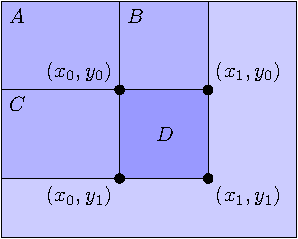
\includegraphics[width=0.3\textwidth]{./slike-latex/ssi}
\end{figure}
%
\subsection{Implementacija in primeri}
\chapter{Generiranje šuma in teksture papirja}
\chapter{Likovno upodabljanje slik}\label{chp:LikovnoUpodabljanjeSlik}
%
Likovno upodabljanje slik (v nadaljevanju LUS) je področje v računalniški grafiki, ki se ukvarja z vprašanjem kako realistični medij slike pretvoriti v artistično likovno delo. V nasprotju z realističnim upodabljanjem, kjer je poudarek na podrobnostih, pri LUS poskušamo upodobiti imanentne informacije. LUS ima zelo široko uporabo pri upodabljanju slik, risb, tehničnih ilustracij, risanih animacij itd. V nasprotju s fotorealističnimi slikami imajo tako dobljena likovna dela namreč to prednost, da lahko likovni umetnik (ali tehnični risar) da poudarek na določen detajl slike, omeji količino podrobnosti, prilagodi paleto barv ali npr.\ doda sliki svojo osebno noto.

LUS se je razvilo iz računalniškega področja prepoznavanja (geometrijskih) oblik na sliki in digitalne obdelave slik. Z razvojem filtrov za obdelavo slik, ki so sprva služili bolj kot npr.~orodje pri tehnični obdelavi medicinskih slik, se je sčasoma njihova uporaba razširila tudi v umetniške vode. Prišlo je do razvoja računalniškega poustvarjanja določenih li\-kov\-ni\-h stilov, kjer so izkoristili lastnosti in delovanje filtrov. 

V prvem razdelku si bomo najprej pogledali primer uporabe filtrov za dosego nekega likovnega efekta na dani fotografiji. Ugotovili bomo, da uporaba filtrov, ki delujejo lokalno, ne pripelje do kompleksnih artističnih efektov. V preostalih razdelkih bomo zato spoznali različne načine za likovno upodabljanje slik, kjer se bomo poslužili modelov čopiča, svinčnika in voščenke ter med drugim uporabljali tudi optimizacijski pristop za slikanje in ustvarjanje mozaikov. V vsakem razdelku bomo navedli nekaj osnovnih člankov in njihovih povzetkov, na podlagi katerih si lahko bralec ustvari predstavo o bogatem dogajanju na področju LUS.
%%
%%
%%
\section{Artistični filter}\label{sec:ArtisticniFilter}
%
Obstaja tudi vrsta komercialnih programov, ki ustvarjajo slike s pomočjo artističnih filtrov, npr.\ Adobe Photoshop.
%%
%%
%%
\section{Tehnične ilustracije}
%
\emph{Tehnična ilustracija} je

\begin{figure}[htb]
  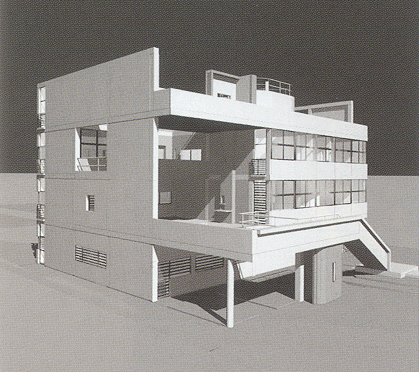
\includegraphics[width=0.49\textwidth]{./slike/real.png}
  \ \ 
  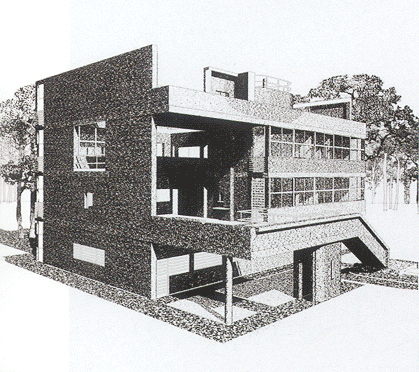
\includegraphics[width=0.49\textwidth]{./slike/npr.png}
  \caption{Razlika med realističnim upodabljanjem in likovnim upodabljanjem.}
\end{figure}
 
Leta 1991 sta Seligmann in Feiner v \cite{Seligmann:Automated} opisala metodo za avtomatično konstruiranje 3D %BAUER Ali je 3D v matematičnem načinu 
ilustracij. Ustvarjanje ilustracij poteka znotraj sistema stilističnih pravil in tehničnih zahtev, ki določajo končni videz ilustracije in jih lahko izbere uporabnik programa. Njun sistem Njihov osnovni cilj je high-level of compositing the best model for comunicatting a particular intent. Yessios je opisal prototip sistema za upodabljanje materialov v arhitekturnih načrtih, kot so kamni, les, rože in tla. Namesto mehaničnega videza želijo ilustracijo prikazati z nežnejšimi potezami. % TODO nežnejšimi ;)
Miyata \cite{Miyata:Stone} je opisal algoritem za upodabljanje vzorcev kamnitih sten. Appel je z soavtorji v \cite{Appel:Haloed} predstavil metodo, s katero narišemo črto, ki ima videz, da gre zadaj za drugo. Kamada in Kawai \cite{Kamada:Hidden} sta posplošila nuno delo in ppredstavila različne parametre črte, kot so črtkanost, pikčastost, \ldots, s pomočjo katerih lahko skrite črte vizualno boljše predstavimo. Dooley in Cohen sta kasneje v \cite{Dooley:Lines, Dooley:Surfaces}  predstavila še več parametrov linij, kot je npr.\ debelina črte in podala diskusijo o načinu uporabnikove interakcije, da bi izboljašlai likovni vtis ilustracij, pri čemer bi obravnavali obliko objekta (linije, ki ga določajo) in njegovo senčenje.

Saito in Takahashi sta v \cite{Saito:3Dshapes} predstavila koncept $G$-bufferja %TODO prevod za G-buffer
za ustvarjanje razumljivih upodobitev 3D scen. Njihova metoda v bistvu po tem, ko ustvarijo množico $G$-bufferjev, uporablja tehnike iz procesiranja slik. V \cite{Wikenbach:ComputerGenerated} sta Winkenbach in Salesin opisala tradicionalne pristope za upodabljanje slik na pen-and-ink način in pokazala, da lahko mnoge izmed njih implementiramo kot del avtomatskega likovnega upodabljanja slik. Predstavila sta stroke texture, % TODO prevedi stroke texture
s pomočjo katerega lahko tako teksturo kot tudi senčenje dosežemo z risanjem linij. Stroke texture dovoljuje tudi likovno upodabljanje slik, ki je odvisno od izbrane resolucije. Opisane tehnike sta demonstrirala s pomočjo kompleksnega arhitekturnega modela, ki vključuje tudi Lloyd's Wright's Robie House. Svoje delo sta v \cite{Winkenbach:ParametricSurfaces} nadgradila, kjer sta uvedla nove algoritme in tehnike za likovno upodabljanje parametrično podanih površin, ki imajo nepravilno obliko. Predstavila sta idejo hatchinga, % TODO hatching - prevod
kjer kontroliramo gostoto risanja linij, da bi dosegli želejeni ton senčenja, obliko in teksturo. Pokazala sta tudi kako lahko ravninski zemljevid, %TODO graf ?
ki je glavna podatkovna struktura pri njunem upodabljanju ilustracij, konstruiramo iz parametrično podanih površin in ga uporabimo za rezanje linij in ustvarjanje linij, ki omejuje objekte. Za ukrivljene objekte sta predstavila tudi senčenje, ki posnema linijo ukrivljenega objekta, ki ga upodabljamo.

Lansdown in Schofield sta v \cite{Lansdown:Expressive} sta predstavila sistem Piranesi, ki uporablja tehnike likovnega upodabljanja za ustvarjanje ilustracij iz podanega 3D modela. Piranedsi uporablja standarne grafične plinovode, % TODO daj link; pipeline
s pomočjo katerih ustvari 2D reliefno sliko. Uporabnik lahko nato posameznim območjim na sliki določi teksturo ali pa je ta določena avtomatsko.

Salisbury je skupaj s sodelavci v \cite{Salisbury:OrientableTextures} predstavil interaktivni sistem za risanje ilustracij na podlagi črnobele vhodne slike, kjer linije na ilustraciji posnemajo obliko objektov na vhodni sliki. Uporabnik, preko novih tehnik za dodajanje vektorskega polja, določi orientacijo za vsako posamezno območje. Računalnik nariše linije, ki temeljijo na uporabnikovih primerih liniji in poskusi doseči iste tone na ilustracji kot so na vhodni sliki, s pomočjo novega algoritma, ki primerja zamegljeno verzijo trenutne ilustracije z vhodno sliko. S poravnanim vektorskim poljem z orientacijami površin objektov na sliki lahko uporabnik ustvari teksturo, ki ima videz, da je pritisnjena na površino, namesto da z njo le potemnimo neketere dele. To ima kot posledico bolj privlačne ilustracije, kot smo jih lahko poprej upodobili iz 2D slik.

Goodwin \cite{Goodwin:IsophoteDistance} s sodelavcama je predstavil pristop za določanje debeline črt v računalniško generiranih ilustracijah gladkih površin. Predpostavka, da se poudarjene črte rišejo na tistih območjih slike kjer je temnejše senčenje, jih je vodila do preproste formule za debelino linij, ki omejujejo objekte in tistih linij, ki sugestirajo detajle na objektih. Formula je odvisna od globine, ukrivljenosti in smeri svetlobe. Za upodabljanje linij uporabijo lokalno obliko in relacijo globine.

\section{Risbe}
Risbe so med osnovnimi likovnimii komunikacijami, ki človeku pomagajo v možganih reproducirati vhodno sliko risbe. Risanje s svinčnikom lahko razdelimo v dve skupini glede na vhodne podatke. te lahko namreč dobimo kot 2D informacijo ali pa kot 3D model. Glavna likovna stila, ki ju s svinčnikom poskušamo upodobiti sta skica ()%TODO povej kaj je skica
in hatching (z risanjem na istem mestu v enakih ali različnih smereh poskušamo doseči določeni ton slike). % TODO prevode
Sousa in Buchanan \cite{Sousa:Model} sta predstavili modele za grafit, papir za risanje, radirke. S temi modeli predstavi  teksturo, ton in %TODO popravi
Modeli so narejeni na podlagi interakcije med grafitom svinčnika in papirja ter na podlagi lastnosti radiranja in smoofanja % TODO kaj je to smufanje ?
S pomočjo parametrov, kot je %TODO iz članka povzetek \cite{Sousa:Polygonal} in \cite{Sousa:Blenders} iz članka ven unga lepega

Lee s sodelavci so v \cite{Lee:RealTime} iz podane 3D površine objekta izločili linije, ki objekt omejujejo in jih predelali za simulacijo ročno narisanih linij. Senčenje simulirajo s pomočjo teksture svinčnika in pa usmerjenih linij. Temelji na svetlobi in materijalu danega 3D modela. Pri upodabljanju slik s svinčnikom so algoritmi najpogosteje taki, da dobijo za vhodni podatek 3D model in nato poskušajo dobiti informacijo o linijah za risbo iz modela \cite{DeCarlo:Photographs, Judd:Ridges, Lee:Abstracted, Grabli:Programmable}. Rusinkiewicz je v \cite{Rusinkiewicz:Review} naredil pregled likovnega upodabljanja s svinčnikom na podlagi danega 3D modela.

V \cite{Lake:Stylized} je bil predstavljen model senčenja. Različne hatching stile sta definirala Hertzmann in Zorin v \cite{Hertzmann:Illustrating}. Praun pa je skupaj sodelavci \cite{Praun:ReaTime} razvil algoritem za hatching, ki se izvaja v realnem času. V \cite{Chen:Example} je predstavljen algoritem za risanje potretov s svinčnikom s stilom, ki posnema določeno tradicijo ali pa stil risarjev.

Mao s sodelavci v \cite{Mao:Automatic} so predstavili postopek za lokalno strukturo orientacije na podlagi vhodne slike in vključili linearno integracijsko konvolucijo (LIC) z namenom simulacije efekta senčenja. Yamamoto pa je s sodelavci v \cite{Yamamoto:Filter} je razdelil vhodno sliko na plasti z različnimi toni v različnih obsegih. Li in Huang \cite{Li:Feature} sta uporabila geometrijske parametre, from ... % TODO lepi članek poglavje 2
%
% TODO kod bodo mozaiki omenjeni
\section{Painterly rendering}
Cohen \cite{Cohen:Aaron, Morbey:Aaron} se je problema risanja oz.\ slikanja lotil z vidika umetne inteligence. Ustvaril je sistem Aaron, ki na podlagi množice randomiziranih pravil ustvari originalno kompozicijo v določenem artističnem stilu. Aaron ima na voljo tudi robotsko slikanje.
  
Haeberli je v \cite{Haeberli:PaintNumbers} predstavil interaktivni sistem za slikanje, ki ustvari impresionistično sliko iz fotografije. Poteze čopiča je upodobil v vrstnem redu. Vsaka poteza je imela parametre (položaj, barva, velikost in oblika), ki so bili večinoma določeni interaktivno, tj.\ s pomočjo uporabnika. Shiraishi in Yamaguchi \cite{Shiraishi:LocalSource} določata orientacijo in obliko potez čopiča na podlagi lokalnih značilnosti vhodne slike. Curtis in ostali avtorji so v \cite{Curtis:Watercolor} predstavili semi-avtomatski algoritem za upodabljanje watercolor slik. %TODO prevod za watercolor
Njihov algoritem ne bo ustvaril vidnih potez čopiča, zato s tem izgubijo artistični vtis slikanja s čopičem. Litwinowicz \cite{Litwinowicz:VideoImpressionist} je opisal avtomatičen sistem za postavitev potez čopiča na podlagi vektorskega polja izračunanega iz gradienta vhodne slike in uporabil rezanje potez na robovih slike. Izhodna slika algoritma je naslikana v impresionističnem stilu, za katerega so značilne kratke poteze. %TODO kam vtaknit to, da je impresionistično
Sistem je razširil na likovno upodabljanje posnetkov. Za upodabljanje posnetkov je uporabil kratke poteze in premikal narisane poteze na platnu s pomočjo izračunanega optičnega toka, ustvarjenega na podlagi posnetka. Pristop, ki ga je Litwinowicz uporabil za postavljanje potez na platno (tj.\ postavitev potez na mrežo) je najbolj pogost način, ki ga uporabljajo za upodabljanje slik s čopičem. Razlike med algoritmi so v obliki in orientaciji potez. Treavett in Chen \cite{Treavett:Statistical} sta predstavila način za likovno upodabljanje s statistično analizo vhodne slike, na podlagi katere določita položaj, orientacijo in velikost upodobljenih potez. Litwinowicz in Treavett s Chenom so sliko pobarvali enoplastno. Pri enoplastnem slikanju je potrebno natančno predviditi položaje in obliko potez, kar pa je težaven problem. Pomankljivost takih algoritmov je torej v tem, da ne moremo morebitnih detajlov in napakic, ki nastanejo pri slikanju ne moremo naknadno popraviti še z eno plastjo potez čopiča. Hertzmann je v \cite{Hertzmann:BrushStrokes} predlagal način upodabljanja slik z večplastnim slikanjem, kjer postavlja na platno poteze čopiča različnih debelin in oblik, ki jih določi s pomočjo Bezierovih krivulj. Začetno točko poteze ne postavi na mrežo slike, temveč v okolici mrežnih točk poišče točko z največjo napako. Kontrolne točke Bezierovih krivulj pa poišče na podlagi izračunanega gradienta vhodne slike. Tak način upodabljanja slikanja je tudi najbolj podobno dejanskemu načinu slikanja. Slikar namreč najprej naredi grobo sliko, ki jo nato z manjšimi čopiči popravi na delih, kjer je potrebno več poudarka in detajlov. S pomočjo te metode lahko ustvarimo sliko, ki ima artistični vtis, vendar pa je potratna in detajlov na sliki vedno ne nariše lepo. To metodo je Hertzmann skupaj s Perlinom razširil na upodabljanje posnetkov \cite{Hertzmann:Video}.

Ročno narisane poteze s čopičem nimajo konstantne barve vzdolž poteze, temveč imajo vgrajeno strukturo. Običajna metoda za upodobljanje potez čopiča je s pomočjo antialiazirane črte, ki ima konststno barvo. Litwinowicz je v \cite{Litwinowicz:VideoImpressionist} predstavil idejo dodajanja teksture in svetlobe pri upodabljanju potez. Hertzmann je v \cite{Hertzmann:Texture} predstavil posebno tehniko za dodajanje efekta svetljenja za likovno upodobljene slike s pomočjo višinskega polja slike in bump-mappinga. %TODO to morš lepo napisat
V \cite{Huang:Natural} so Huang in sodelavci predstavili podoben način kot je bump-mapping, vendar je bistveno enostavnejši za implementacijo. Predstavili so model anizotropičnega čopiča. Upodobaljanje potez poteka tako, da pripravljeno masko čopiča (na podlagi ...)%TODO napiši še kaj

Hays in Essa sta v \cite{Hays:Animation} predstavila uniform %TODO uniform kot kaj
likovno upodabljanje za slike in posnetke. Za razliko od večine prejšnjih algoritmov, so poteze pri tej metodi postavljene na večjem platnu. Orientacije za poteze so izračunane z RBF interpolacijo. Pri upodabljanju posnetkov, se parametri potez med postopkom spreminjajo, orientacija potez pa je določena z vektorskim poljem na podlagi gradienta posameznih sličic, različne frekvence robov na sliki pa pripomorejo h upodobitvi detajlov na sliki.

%TODO manjka še tazadni del, pa pejd po novem članku

Uporaba informacije o 3D geometrijski strukturi slike, ki jo želimo likovno upodobiti, nam dovoljuje veliko več fleksibilnosti pri ustvarjanju posnetkov. Meier iz Walt Disney Feature Animation je %TODO povej da je Disney
v \cite{Meier:Animation} predstavila avtomatičen sistem, ki postavlja poteze čopiča na podlagi opisa posameznih delov slike. %TODO preberi kaj naredi
V filmih \textit{Tarzan} \cite{Daniels:Tarzan} in \textit{What Dreams May Come} %TODO daj imbd linke
so bile uporabljene razširitve tega algoritma.  Tak sistem naravno zagotavlja časovno koherenco in ekonomičnost likovnega upodabljanja posnetka. Vendar pa podatki o geometrijski strukturi niso vedno dosegljivi. Klein \cite{Klein:Virtual} je objekte upodobil s pomočjo filtrirane strukture. % TODO poglej si
Uporaba 3D strukture tipično proizvede drugačen srtistični učinek, saj so poteze čopiča vezane na geometrijsko struktuo objektov. Turk in Banks sta v \cite{Turk:Guided} za ilustriranje vektorskega polja z uporabila relaksacijo. Njuno delo in uporabo relaksacije, ki jo je uporabil Haeberli v \cite{Haeberli:PaintNumbers}, je Hertzmann razširil v članku \cite{Hertzmann:Relaxation}.

Lee je v \cite{Lee:Motion} predstavil novo metodo za za določanje oprientacije potez čopiča v likovnem upodabljanju posnetkov. Informacijo o premikih, ki jo dobimo iz zaporedja sličič posnetka uporabimo za orientiranje potez čopiča v območjih, kjer je bilo zaznano večje gibanje. %TODO v uvodu splošnem že povej, da so pri upodabljanjih videjov problem šum
V območjih z rahlio zaznanim gibanjem pa določimo orientacijo potez čopiča na podlagi gradienta slike. % TODO I guess
Določanje orientacije po tem postopku ima prednost pri izražanju gibanja objektov. 
\include{./poglavja/SlikanjeSCopicem}
\chapter{Risanje z voščenkami}
%
V članku \cite{DRudolf:BiWaxCrayon} predstavljeni postopek likovnega upodabljanja risanja z voščenkami modelira risanje na podlagi fizikalnih modelov, ki so bili eksperimentalno določeni in preizkušeni. Delu voščenke s katerim rišemo po papirju pravimo \emph{profil}. Voščenke so zgrajene iz mehkega in viskoznega materiala ter imajo standardni premer $8~mm$ (standardni večji premer meri $11~mm$). Zaradi velikosti profila pri stiku voščenke z risalnim papirjem ne smemo privzeti, da se profil spreminja homogeno na celotni površini, temveč moramo obravnavati spreminjanje profila na mikroravni. Pri risanju z voščenkami je pomemben začetni profil voščenke, ki vpliva na kasnejše spreminjanje profila, ko se material na profilu zaradi hrapavosti papirja neenakomerno kruši v plasteh.

Najprej bomo v prvem razdelku določili podrobnejše modele za voščenke in risalni papir, ki jih bomo uporabili v algoritmu. V drugem razdelku bomo predstavili ogrodje glavnega algoritma za likovno upodabljanje z voščenkami ter definirali potrebne pojme in (fizikalne) količine, ki jih bomo potrebovali. Pri eksperimentalnih poskusih je bilo opaženo, da pri risanju z voščenko na delu papirja, kjer je že bila nanešena plast voska, star nanos voska v smeri risanja potisnemo v sosednje območje, nekaj pa se ga lahko prime tudi nazaj na profil \ldots Ta opažanja bomo fizikalno opisali in predstavili algoritme za njihovo simulacijo. V naslednjem razdelku bomo s pomočjo KM barvnega modela, predstavljenega v \ref{chap:KMModel}, in eksperimentalno določenih parametrov za barve otroških voščenk predstavili končni algoritem, ki bo vrnil risbo narisano z voščenkami.

V zadnjem razdelku bomo opisali našo implementacijo algoritma in poskusno naredili slike z voščenkami, pri katerih uporabnik kot vhodni podatek ne bo podal skice v izbranih barvah za voščenke kot v članku, temveč bo podal (barvno) sliko, na podlagi katere bo program določil linije, ki jih bo pobarval z naračunanimi barvami voščenk.
%
\section{Model voščenke in papirja}
%
\subsection{Model voščenke}
%
Profil voščenke modeliramo kot dvodimenzionalno višinsko masko $M$, pri čemer vrednost posamezne celice $m_{i, j} \in M$ predstavlja pravokotno oddaljenost $h_{m_{i,j}}$ pripadajoče točke na profilu voščenke od \emph{osnovne ravnine} na kateri leži risalni papir. Maska $M$ mora biti dinamična, saj se pri risanju profil spreminja zaradi luščenja voska. Spreminjanje maske bomo opisali pri obravnavi algoritma.

Uporaba dinamične maske nam omogoča izbiro poljubnega začetnega profila voščenke. Za profile voščenk, pri katerih kot pravokotno projekcijo na osnovno ravnino dobimo krog, pravimo, da so \emph{okrogli profili}. Za slednje pravimo, da imajo \emph{polmer $R$}, kadar je premer voščenke enak $2\cdot R + 1$ (dodatna ena celica je tu iz tehničnih razlogov, saj pri implementaciji lažje operiramo z maskami lihe velikosti). Na sliki~\ref{fig:maske-voscenke} so prikazani nekateri možni profili, ki jih lahko uporabimo pri modeliranju risanja z voščenkami.

%
\begin{figure}[htbp]
  \centering
  \subfigure[]{
  
\includegraphics[width=0.2\textwidth]{./slike/wax}
  \ \ \ \ 
  \includegraphics[width=0.2\textwidth]{./slike/profil}
   }
   \ \ \ \ 
  \subfigure[]{
  
\includegraphics[width=0.2\textwidth]{./slike/waxp}
  \ \ \ \ 
  
\includegraphics[width=0.2\textwidth]{./slike/profilp}
  }
  
  \subfigure[]{
  
\includegraphics[width=0.2\textwidth]{./slike/waxkot}
  \ \ \ \ 
  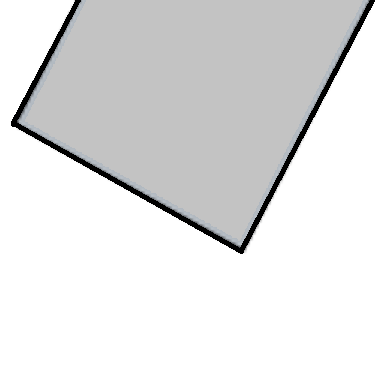
\includegraphics[width=0.2\textwidth]{./slike/profilkot}
  }
  \ \ \ \ 
  \subfigure[]{
  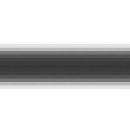
\includegraphics[width=0.2\textwidth]{./slike/waxl}
  \ \ \ \ 
  
\includegraphics[width=0.2\textwidth]{./slike/profill}
  }
  \caption{Prikaz modelov za nekatere možne profile voščenke. Standardni profil voščenke je prikazan zgoraj levo. Intezitete slikovnih točk ustrezajo vrednostim $h_{m_{i,j}}$.}
  \label{fig:maske-voscenke}
\end{figure}
%

Celicam maske $M$ predpišemo tudi statično vrednost $u_{m_{i,j}}$, ki je sorazmerna deležu površine celice $m_{i,j}$, ki leži znotraj območja pravokotne projekcije profila na osnovno ravnino. Vrednost $u_{m_{i,j}}$ poimenujemo \emph{utež celice $m_{i,j}$}, za masko $M$ pa pravimo, da je \emph{utežena}. Z uporabo utežene maske se izognemu pojavu kvadratkastega videza končne slike (kar se pri dejanski izvedbi algoritma izkaže kot težava, še posebej pri uporabi profila voščenke na sliki \ref{fig:maske-profil3}, kadar voščenko nagnemo pod kotom manjšim od $20 \degree$). Na sliki \ref{fig:utezena-maska} je prikazan primer utežene maske okroglega profila voščenke s polmerom 6.

%
\begin{figure}[htbp]
  \centering
  \subfigure[]{
  
\includegraphics[width=0.2\textwidth]{./slike-latex/area.pdf}
  }
  \subfigure[]{
  
\includegraphics[width=0.2\textwidth]{./slike-latex/area-utez}
  }
  \caption{Prikaz modelov za nekatere možne profile voščenke. Standardni profil voščenke je prikazan zgoraj levo. Intezitete slikovnih točk ustrezajo vrednostim $h_{m_{i,j}}$.}
  \label{fig:maske-voscenke}
\end{figure}
%
\subsection{Model papirja}
%
\section{Modeliranje risanja z voščenkami}
%
Pri eksperimantalnih poskusih risanja z voščenkami opazimo, da se vosek s profila prenese na risalni list v neenakomernih plasteh in posledično spremeni obliko profila. Nadalje opazimo, da se vosek, ki je že nanešen na risalnem listu, če gremo ponovno preko njega z voščenko, prenese v sosednja lokalna območja v trenutni smeri risanja. Obravnava na mikroravni pokaže, da se prenese predvsem tisti del vosek, ki se nahaja na vrhih risalnega lista, in sicer v bližnje doline (glej siko \ref{fig:prenos-voska}). Prav tako pa se lahko manjša količina voska prime nazaj na profil.

%
\begin{figure}[htbp]

\includegraphics[width=0.2\textwidth]{./slike-latex/area.pdf}
\end{figure}
%
\subsection{Osnovne količine in algoritem za risanje posameznih linij}
%
Risanje posameznih linij simuliramo z algoritmom \ref{alg:glavniVoscenke}.

%
\begin{algorithm}[hbt]
  \caption{Povzetek glavnega algoritma za risanje z voščenkami.}
  \label{alg:glavniVoscenke}
\begin{algorithmic}[1]
\Require $P_1$, $P_2$, $M$, $C$, $f$, $L$
\Ensure Nova poteza z voščenko.
\Function {NovaLinija} {$P_1$, $P_2$, $M$, $C$, $f$, $L$}
  \For {$P_i \in \vec{P_1P_2}$} % TODO stavek \In
    \State \Call {PrilagodiVoščenko} {$P$, $M$, $f$, $L$}
    \State \Call {Redepozicija} {$P$, $\vec{V}$}
    \State \Call {Smearing} {$P_i$, $\vec{P_1P_2}$, $M$, $L$}
    \State \Call {DodajVosek} {$P_i$, $\vec{P_1P_2}$, $f$, $M$, $C$, $L$}
  \EndFor
\EndFunction
\end{algorithmic}
\end{algorithm}
%

Vhodni podatki algoritma so:
%
  \begin{itemize}
  \item $P_1, P_2$ $\ldots$ začetna in končna točka linije, ki jo bomo narisali,
  \item $M$ $\ldots$ maska profila voščenke,
  \item $C$ $\ldots$ barva voščenke,
  \item $f$ $\ldots$ velikost sile s katero pritiskamo voščenko na risalni list pri risanju,
  \item $L$ $\ldots$ seznamov posameznih nanosov voska (višina nanosa in njegova barva) za vsako slikovno točko na papirju.
  \end{itemize}
%
\subsection{Prilagoditev profila voščenke}
Na količino voska, ki se bo odluščil s profila, vplivajo naslednji dejavniki:
%
  \begin{itemize}
  \item površina profila,
  \item velikost in smer sile s katero pritiskamo voščenko pri risanju,
  \item relativna oddaljenost profila od risalnega lista,
  \item lokalna tekstura risalnega lista na trenutnem območju, kjer je profil voščenke.
  \end{itemize}
%
Pri risanju z voščenko se s profila lušči vosek, kar pomeni, da se veča skupna oddaljenost profila od ravnine risalnega papirja. Ker ohranjamo silo $f$ konstantno vzdolž ene linije, to pomeni, da bi na neki točki lahko izgubili stik med profilom in risalnim listom. Da se temu izognemu, bomo na vsakem koraku na novo prilagodili višino in obliko profila. Ob privzetku, da se dolžina voščenke zmanjšuje linearno, si bomo pri prilagajanju višine profila pomagali s Hookovim zakonom o kompresiji.
%
\subsubsection{Hookov zakon}
Hookov zakon lahko zapišemo v obliki
$$F = Y \frac{\Delta L}{L_0} A,$$
kjer so $Y$ Youngova konstanta modula, $\Delta L$ konstanta za stiskanje, $L_0$ nestisnjena dolžina voščenke in $A$ velikost profila. Ob privzetku, da je dolžina voščenke $L_0$ približno konstantna ($L_0 >> \Delta L$), lahko uvedemo novo konstanto $\lambda$, s katero se Hookov zakon prepiše v obliko:
%
\begin{equation}\label{eq:Hook2}
F = \lambda A \Delta L.
\end{equation}
%
Za konstanto $\lambda$ izberemo vrednost, ki nam bo dala estetsko primerne rezultate.
%
\subsubsection{Prilagoditev višine voščenke}
Kot smo že omenili, je zaradi velikosti površine profila, potrebna obravnava profila na mikroravni. V ta namen bomo po formuli \eqref{eq:Hook2} izračunali za vsako posamezno celico maske $m_{i,j} \in M$ prispevek k celotni sili: $F_{m_{i,j}} = \lambda \delta h$ ($A = 1$ za vsako celico profila). V primeru, ko med celico profila in istoležno točko na risalnem papirju ni stika (celica profila leži nad istoležno točko na risalnem listu), prispevek k sili nastavimo na 0. Skupna sila $F$ je enaka vsoti posameznih prispevkov, $F = \sum_{m_{i,j}} F_{m_{i,j}}$.

Količina $\delta h$ je v tem primeru razlika med višinama celice profila in istoležne točke na risalnem papirju skupaj z že nanešenim voskom. Višina celice profila bo tu odvisna od višine voščenke $h$, posledično je torej $F$ funkcija spremenljivke $h$, $F(h)$. Dobili smo aproksimacijski problem, pri katerem želimo čimbolje aproksimirati velikost sile $f$. Ker je $F$ vsota posameznih prispevkov, funkcija $F(h)$ ni več zvezna, lahko pa jo opišemo kot deloma zvezno funkcijo. Pri aproksimaciji si bomo pomagali z Newtonovo metodo. Natančnost aproksimacije in same simulacije pa nadziramo s konstanto napake $\varepsilon$. Eksperimentalno opazimo, da uporaba večje napake pohitri Newtonovo metodo, še vedno pa nam da likovno zadovoljive rezultate. V algoritmu \ref{alg:adjustCrayonHeight} je podana psevdokoda za določitev nove višine voščenke.

%
\begin{algorithm}[htb]
  \caption{Prilagoditev voščenke.}
  \label{alg:adjustCrayonHeight}
\begin{algorithmic}[1]
\Require $P$, $M$, $f$, $L$
\Ensure Spremenjena maska voščenke.
\Function {PrilagoditevVoščenke} {$P$, $M$, $f$, $L$}
  \State $h_{min}^{vo"s"cenka}$ $\gets$ $\displaystyle \min_{m_{ij} \in M} h_{m_{ij}}$
  \State $h_{min}$ $\gets$ $\displaystyle \min_{m_{ij} \in M} h_{P_{ij}}$ \Comment $P_{ij} = P + (i, j)$
  \State $h_{max}$ $\gets$ $\displaystyle \max_{m_{ij} \in M} h_{P_{ij}}$
  \While {$h_{max} - h_{min} > \Delta$}
    \State $h_{mid}$ $\gets$ $(h_{max} - h_{min})/2$
    \State $\getvalue{f_{mid}}{0}$
    \ForAll {$m_{ij} \in M$}
      \State $\delta h = h_{P_{ij}} + h_{L_{P_{ij}}} - (h_{m_{ij}} - h_{min}^{vo"s"cenka} + h_{mid})$
      \If {$\delta h > 0$}
        \State $\getvalue{f_{mid}}{\lambda \delta h}$
      \EndIf
      \If {$f < f_{mid}$}
        \State $\getvalue{h_{min}}{h_{mid}}$
      \Else
        \State $\getvalue{h_{max}}{h_{mid}}$
      \EndIf
    \EndFor
    \State $\getvalue{h_{mid}}{(h_{min} + h_{max})/2}$
    \ForAll {$h_{m_{ij}}$}
      \State $\getvalue{h_{m_{ij}}}{h_{m_{ij}} - h_{min}^{vo"s"cenka} + h_{mid}}$
    \EndFor
  \EndWhile
\EndFunction
\end{algorithmic}
\end{algorithm}
%

\subsection{Trenje}
Pri risanju z voščenko se bo zaradi mehkobe materiala iz katerega je zgrajena voščenka in trenja, ki nastane med voščenko in papirjem, vosek razporedil naokoli. %TODO a se reče mehkobe ali zakaj ...?
Trenje med voščenko in papirjem bomo opisali na makro in mikro ravni. Na makro ravni nas zanima normalna sila voščenke na površino papirja. Če voščenka preide mimo konveksnega % TODO konveksno za fizike
delčka v teksturi papirja, se bo od voščenke odstranil del voska, ki bo ostal za tem konveksnim delčkom papirja. Na mikro ravni uporabimo koeficient trenja, da aproksimiramo hrapavost papirja na manjši skali. Želimo, da je količina prestrukturiranega voska sorazmerna s silo trenja, ki je definirana kot
$$
\vec{F_F} = \mu \vec{F_N} = \mu \vec{N} \frac{\vec{N} \cdot \vec{F_C}}{\norm{\vec{N}} \norm{\vec{F_C}}}, %TODO wtf je s temi normami ???
$$
kjer je $\vec{F_C}$ sila voščenke na površino papirja, $\vec{F_F}$ je sila trenja, $\vec{F_N}$ je normala sile trenja na površino papirja, $\vec{N}$ je normala na površino papirja in $\mu$ je koeficient trenja papirja pri stiku z voščenko. % TODO ali se reče, da ima papir trenje, ali je trenje med papirjem in pa voščenko

Na podlagi teksture papirja interpoliramo sosednje vrednosti višin celic papirja, da dobimo ravnino po kateri se voščenka premika, in izračunamo silo trenja. Sila trenja je odvisna od naračunane ravnine, dane konstante sile trenja voščenke na papir in smeri risanja z voščenko.

Vrednost $\mu$ je odvisna od tega ali rišemo na čist papir ali pa je ta že porisan. Še več, območje papirja na katerem je debelina nanešenega voska voščenke večja, bo imelo drugačne lastnosti in trenje kot območja papirja s tanjšim slojem nanešenega voska voščenke. %TODO nanešenega ni v sskj ?
Če bi želeli biti rigorozni pri simulaciji trenja med voščenke in papirja, bi morali upoštevati zgornje. Vendar pa zaenkrat nimamo še rezultatov, ki bi povedali vrednost koeficienta za trenje papirja, ki bi dal rezultate kot bi jih želeli. Na področju teg bla bla \ref{24, 25} % TODO povej da mi bomo to kar malo tko naredli pa poglej še v članek nazaj; pa spiši neki
Pri naši simulaciji bomo določili posebej koeficient trenja za voščenko $\mu_{vo"s"cenka}$ in papir $\mu_{papir}$. Koeficient trenja bomo izračunali sproti kot linearno kombinacijo $\mu_{vo"s"cenka}$ in $\mu_{papir}$ na podlagi trenutnega faktorja.

V algoritmu \ref{alg:addNewWax} je podana psevdokoda za risanje z voščenko z upoštevanjem trenja.

%
\begin{algorithm}[htb]
  \caption{Risanje z voščenko in računanje trenja med voščenko in papirjem.}
  \label{alg:addNewWax}
\begin{algorithmic}[1]
\Require $P$, $\vec{V}$, $M$, $C$, $f$, $L$
\Ensure Dodan vosek. %TODO neki si zmisli, da bo tuki pisalo nekaj drugega kot izhodni podatki, ker to izhodni podatki v resnici niso
\Function {DodajVosek} {$P$, $\vec{V}$, $M$, $C$, $f$, $L$} % TODO neumno ime
  \State $\getvalue{\vec{V}}{\vec{V}/\max (x_{\vec{V}}, y_{\vec{V}})}$
  \ForAll {$m_{ij} \in M$}
      \State $\getvalue{P_{ij}}{P + (i, j)}$
      \State $\getvalue{\hat{P}_{ij}}{P_{ij} + \vec{V}}$
      \State $\getvalue{\vec{S}_{ij}}{(x_{\vec{V}}, y_{\vec{V}}, -h_{P_{ij}})}$
      \State $\getvalue{\vec{F}_{ij}}{(x_{\vec{V}}, y_{\vec{V}}, -f)}$
      \State $\getvalue{\vec{F}_{ij}}{1/(1 + h_{\hat{P}_{ij}}^{vo"s"cenka})}$
      \State $\getvalue{\mu_{ij}}{\alpha \mu_{papir} + (1 - \alpha) \mu_{vo"s"cenka}}$
      \State $\getvalue{\delta h_{\hat{P}_{ij}}^{vo"s"cenka})}{\mu (h_{\hat{P}_{ij}} - h_{m_{ij}}) \sin (\vec{S}_{ij}, \vec{F}_{ij})}$
      \State $\getvalue{h_{m_{ij}}}{h_{m_{ij}} + \delta h_{\hat{P}_{ij}}^{vo"s"cenka})}$ %TODO tile left{ right} se weird obnašajo - enormno veliki :(
      \State $\getvalue{L_{P_{ij}}}{L_{P_{ij}} + \set{(\delta h_{\hat{P}_{ij}}^{vo"s"cenka}), C)}}$
  \EndFor
\EndFunction
\end{algorithmic}
\end{algorithm}
%
%%
\section{Smearing}
Smearing je lastnost voščenke, podobno kot je krvavanje pri čopiču. % TODO krvavenje ni okej, neki drugega si zmisli
Pri risanju z voščenko na območjih z že nanešenim voskom voščenke, se vosek porazdeli in potisne bolj noter v luknje. % TDOo popravi to
Za simulacijo smeraringa bomo najprej uvedli smearing masko, ki upošteva trenutno točko in njene sosede. Vrednosti v maski voščenke določajo količino voska, ki se bo prenesel izpod trenutne točke in raznesel naokoli. Pri tem torej upoštevamo točko in njenih osem sosedov. Zaradi mehkobe materiala voščenke, predpostavimo,da je to dovolj upošteavti, medtem ko za nekatere druge materiale to ne bi bilo res (npr.\ pastelne barvice).
 
Pri simulaciji si bomo pomagali s filtrom $S$ velikosti $3 \times 3$. Elemente filtra izračunamo s formulo
$$S_{xy} = \frac{1}{\norm{(\vec{x, y})}} (\alpha \Delta z + \beta (\widehat{x, y}) \cdot \hat{V}).$$
Vrednost celice $S_{xy}$ nastavimo na 0, preprečimo morebitni prenos voska nazaj na voščenko. % TODO razmisli

V algoritmu \ref{alg:smearing} je podana psevdokoda za postopek smearinga.

%
\begin{algorithm}[htb]
  \caption{Smearing.}
  \label{alg:smearing}
\begin{algorithmic}[1]
\Require $P$, $\vec{V}$, $M$, $L$
\Ensure Posmearan papir.
\Function {Smearing} {$P$, $\vec{V}$, $M$, $L$} % TODO prevod
  \State $\getvalue{\vec{V}}{\vec{V}/\max (x_{\vec{V}}, y_{\vec{V}})}$
  \ForAll {$m_{ij} \in M$}
      \State $\getvalue{P_{ij}}{P + (i, j)}$
      \State $\getvalue{\hat{P}_{ij}}{P_{ij} + \vec{V}}$
      \State $\getvalue{\vec{S}_{ij}}{(x_{\vec{V}}, y_{\vec{V}}, -h_{P_{ij}})}$
      \State $\getvalue{\vec{F}_{ij}}{(x_{\vec{V}}, y_{\vec{V}}, -f)}$
      \State $\getvalue{\vec{F}_{ij}}{1/(1 + h_{\hat{P}_{ij}}^{vo"s"cenka})}$
      \State $\getvalue{\mu_{ij}}{\alpha \mu_{papir} + (1 - \alpha) \mu_{vo"s"cenka}}$
      \State $\getvalue{\delta h_{\hat{P}_{ij}}^{vo"s"cenka})}{\mu (h_{\hat{P}_{ij}} - h_{m_{ij}}) \sin (\vec{S}_{ij}, \vec{F}_{ij})}$
      \State $\getvalue{h_{m_{ij}}}{h_{m_{ij}} + \delta h_{\hat{P}_{ij}}^{vo"s"cenka})}$ %TODO tile left{ right} se weird obnašajo - enormno veliki :(
      \State $\getvalue{L_{P_{ij}}}{L_{P_{ij}} + \set{(\delta h_{\hat{P}_{ij}}^{vo"s"cenka}), C)}}$
  \EndFor
\EndFunction
\end{algorithmic}
\end{algorithm}
%
%%
\section{Redepozicija}
Ena izmed lastnosti voščenk je tudi ta, da se vosek, ko prečkamo območje, na katerem smo predhosno že nanesli plast voska, vosek nanese nazaj na voščenko. Pri premikanju voščenke po papirju se vosek, ki je že nanešen odkruši s papirja in lahko gre nazaj na voščenko ter se nato z voščenko prenese na drugo območje na papirju. Podoben problem je pri risanju s čopičem \ref{18, Baxter}. %TODO opis tega baxterja, neki je not v članku, mal bla bla

Zaradi viskoznosti materiala voščenke, se pigmenti v voščenki ne mešajo tako kot pri barvi, temveč se plasti voščenke odluščijo s papirja in pritisnjeo nazaj na voščenko. Ta vosek bo bil razporejen naokoli linearno in ne eksponentno. Barva s čopiča se prične mešati z barvo na platnu takoj ob stiku čopiča s platnom. Medtem, ko se pri voščenki nič voska ne bo razporedilo zgolj samo pri stiku.Z voščenko moramo podrgniti vosek iz papirja.

V algoritmu \ref{alg:reclaimWax} je povzeta psevdokoda za redepozicijo voska.

%
\begin{algorithm}[htb]
\caption{Redepozicija voska.}
\label{alg:reclaimWax}
\begin{algorithmic}[1]
\Require $P$, $\vec{V}$, $M$, $L$, $f$
\Ensure Razporejen vosek.
\Function {Redepozicija} {$P$, $\vec{V}$, $M$, $L$, $f$}
  \ForAll {$m_{ij} \in M$}
    \State $\getvalue {S} {3 \times 3 \text{ smearing mask}}$
      \ForAll {$s_{qr} \in S$}
        \State {$s_{qr}$} {$\max\set{0, \vec{V} \cdot \hat{(q, r)}}$}
      \EndFor
      \State $\getvalue {S} {\gamma f S / (\sum s_{qr})}$
      \State $\getvalue {\delta h_{vo"s"cenka}} {\max \set{0, h_{m_{i+q, j+r}} - h_{m_{ij}}}}$
      \State $\getvalue {L_{P_{ij}}'} {\set{l_a, \ldots, l_n} : \sum h_{l_i} \leq \delta h_{vo"s"cenka}}$
      \State $\getvalue {L_{P_{ij}}} {L_{P_{ij}} - L_{P_{ij}}'}$
      \ForAll {$s_{qr} \in S$}
        \ForAll {$l_k \in \delta L_{P_{ij}}'$}
          \State $\getvalue {m_{i+q, j+r}} {m_{i+q, j+r} + s_{qr} l_k}$
        \EndFor
      \EndFor
  \EndFor
\EndFunction
\end{algorithmic}
\end{algorithm}
% 
%%
\section{Upodabljanje z voščenkami}
Vosek je najlažje obravnavati kot prosojen pigment, za kar sta enostavna modela RGB in CMY pomankliva, da bi ju lahko uporabili. Namesto tega bomo uporabili Kubelka-Monk barvni model \ref{21}. KM model aproksimira spektralno prosojnost, sipanje in motnje. Vrednosti teh lastnosti lahko določimo s pomočjo dveh barv \ref{9}. Vsaka izmed teh barv je opaženi rezultat nanešene plasti na enobarvno ozadje (uporabimo belo in črno ozadje). Iz teh dveh barv KM model nato interpolira ti dve vrednosti, da dobi vrednosti za poljubne debeline nanešenega voska na ozadje katerekoli barve. KM model naredi to tako, da predvidi količino sipanja svetlobe glede na material pigmenta, in koliko je ta material prosojen. KM model aproksimira tudi spremembe, ki nastanjeo zaradi tankih motenj.

V našem modelu, ki ga bomo uporabili za risanje z voščenkami, bomo zanemarili motnje, saj v eksperimntalnih poskusih ni zaznati bistvenega vpliva. Posledično je vsaka voščenka predstavljena z enim naborom RGB barv ter parametrom prosojnost in sipanje.

Kot smo že omenili prej zelo tanke plasti voščenke združimo skupaj. Optične lastnosti končne plasti nastavimo na uteženo povprečje združenih plasti. Vsak prispevek plasti h končni plasti je torej sorazmeren z njegovo višino. To je groba peonostavitev KM modela, vendar še vedno da sprejemljive rezultate in bistveno zmanjša čas, ki je potreben za smearing.

Za upodobitev slike z voščenkami moramo vsaki točki na papirju $P_{ij}$ pripisati barvo $C_{P_{ij}}$. Za izračun barve, ki jo dobimo za plast $l_k \in L_{P_{ij}}$, uporabimo barvo plasti $C_{l_k}$, njeno prosojnost $t_{l_k}$ in sipanje $r_{l_k}$.

V algoritmu \ref{alg:render} je podana psevdokoda za upodabljanje slik z voščenkami.

%
\begin{algorithm}[htb]
\caption{Algoritem za upodabljanje slik z voščenkami.}
\label{alg:render}
\begin{algorithmic}[1]
\Require $T$
\Ensure Slika narisana z voščenkami.
\Function {Upodabljanje} {$T$}
  \ForAll {$P_{ij}$ teksture papirja $T$}
    \State $\getvalue {C_{ij}} {C_{P_{ij}}}$
    \ForAll {plasti voska $l_k$ v točki $P_{ij}$}
      \State $\getvalue {C_{ij}^{prosojnost}} {(t_{l_k} C_{l_k})^{h_{l_k}} C_{ij}}$
      \State $\getvalue {C_{ij}^{sipanje}} {1 - (1 - C_{l_k})^{r_{l_k} h_{l_k}}}$
      \State $\getvalue {C_{ij}} {C_{ij}^{prosojnost} + C_{ij}^{sipanje}}$
    \EndFor
  \EndFor
\EndFunction
\end{algorithmic}
\end{algorithm}
%
Eksperimentalno smo določili osnovne barve vočenk in njihove parametre. Podani so v tabeli \ref{tbl:voscenke}.

% TODO v novem članku so drugačne vrednosti !!!
\begin{table}[htb]
\begin{tabular}{ll|lll|ll}
\hline
Voščenka & Barva & R & G & B & t & s \\
\hline
& rdeča & 0.95 & 0.45 & 0.45 & 0.605 & 0.0425 \\
& oranžna & 0.999 & 0.55 & 0.3 & 0.77 & 0.03 \\
& rumena & 0.95 & 0.9 & 0.2 & 0.869 & 0.0425 \\
& zelena & 0.35 & 0.8 & 0.35 & 0.55 & 0.06 \\
& modra & 0.3 & 0.5 & 0.9 & 0.77 & 0.045 \\
& vijolična & 0.65 & 0.45 & 0.75 & 0.715 & 0.05 \\
& rjava & 0.8 & 0.6 & 0.55 & 0.495 & 0.075 \\
& črna & 0.26 & 0.25 & 0.245 & 0.935 & 0.05 \\
& siva & 0.42 & 0.4 & 0.39 & 0.594 & 0.275 \\
& bela & 0.8 & 0.8 & 0.78 & 0.88 & 0.175 \\
& periwinkle & 0.7 & 0.7 & 0.9 & 0.605 & 0.125 \\
& morsko zelena & 0.6 & 0.9 & 0.65 & 0.55 & 0.1 \\
& orhideja & 0.85 & 0.4 & 0.84 & 0.88 & 0.075 \\
\hline
\end{tabular}
\caption{Tabela z vrednostmi za barve, ki jih uporabljajo otroci (povzeto po članku \ref{voscenke}).}
\label{tbl:voscenke}
\end{table}
%
\chapter{Risanje s svičnikom}
V zadnjem poglavju bomo predstavili algoritem za risanje s svinčnikom. Osnova naše implementacije algoritma bo temeljila na članku \cite{}, ki ga bomo prilagodili in dopolnili z nekaterimi dodatnimi koraki iz članka \cite{}.

Kot smo videli že v razdelku \ref{}, lahko pristopimo k risanju s svinčnikom na več načinov. V članku \cite{} predstavljeni postopek risanja sodi v kategorijo risarskih postopkov, kjer senčenje izvedemo tako, da ustvarimo zvezno območje sivine, ki vsebuje teksturo, z linijskimi črtami pa poudarimo linije, ki dajo objektom na sliki obliko. Predstavljeni postopek risanja s svinčnikom v tem članku bomo razdelili v tri faze:
%
\begin{enumerate}
  \item zaznava linij na sliki in izračun linijske slike $\tilde{S}$;
  \item izračun sivinske slike $T$;
  \item kompozicija linijske in sivinske slike v skupno risbo $R$.
\end{enumerate}
%
Posamezne faze bomo predstavili v prvih treh razdelkih, v zadnjem razdelku pa bomo opisali našo implementacijo tega algoritma in njegovo analizo skupaj z dodatnimi primeri.
%
\section{Linijska slika}
Pri risanju s svinčnikom risarji uporabljajo kratke linijske črte. Dolge linijske črte na risbi narišejo kot zaporedje krajših, ki se na koncih nekoliko križajo. Podoben pristop bomo izbrali v našem algoritmu za izračun linijske slike. Končni rezultat, ki ga bomo dobili, bo neosenčena skica vhodne slike.

Za izračun linijske slike bomo morali na vhodni sliki zaznati linije, ki jih želimo narisati, določiti njihov položaj, dolžino, odtenek sivine in debelino. Zaradi prisotnosti teksture in šuma na vhodni sliki, običajni filtri za zaznavo robov na sliki, npr.\  Sobelov filter, ne bodo zadostili likovnim kriterijem. Zato bomo pripravili lastne filtre, ki bodo dali zadovoljiv rezultat tudi v primeru prisotnosti teksture in šuma. V nadaljevanju bomo opisali posamezne korake v algoritmu za risanje linij in jih opremili s primeri.
%
\subsection{Classification}
Vhodno (barvno) sliko moramo najprej pretvoriti v sivinsko sliko $I$. Uporabimo lahko standardno sivinsko pretvorbo ali pa naredimo svetlostno pretvorbo. % Oboje je definirano nekje v razdelku Barvni modeli.
Eksperimentalno se izkaže, da uporaba svetlostne pretvorbe ponuja boljše izhodišče za zaznavo robov na sliki, zato bomo v našem algoritmu izbrali to pretvorbo. Na dobljeni sliki $I$ bomo nato uporabili še filter za izostritev robov, ki bo linije na sliki naredil bolj izrazite.

Podobno kot v razdelku \ref{sec:filtri}, ko smo izpeljevali filter za zaznavo robov, bomo tudi sedaj s pomočjo gradientnih slik v $x$ in $y$ smereh ($\partial_x I$ in $\partial_y I$) izračunali gradientno sliko
%
$$G \coloneqq \sqrt{(\partial_x I)^2 + (\partial_y I)^2} \;.$$
%
Kot smo videli pri filtrih za zaznavo robov, znajo ti zaznati robove v treh smereh (vodoravno, navpično, diagonalno), kar pa z likovnega stališča ni zadostno. Pri risanju namreč linijske črte rišemo v poljubnih smereh. Zato bomo definirali množico pomožnih filtrov $\L_n = \set{\LL_i}_i^n$, ki bodo znali zaznati robove v $n$ smereh (posledično bomo znali narisati linijske črte v teh $n$ smereh). Posamezen filter predstavlja linijsko črto v $i$-ti smeri z dolžino, ki je sorazmerna z velikostjo vhodne slike. V našem algoritmu bomo uporabili 4 oz.\ 8 različnih smeri, imeli bomo torej $\L_4 = \set{\LL_1, \LL_2, \LL_3, \LL_4}$ oz.\ $\LL_8 = \set{\LL_1, \LL_2, \ldots, \LL_8}$. Velikost filtrirnih matrik bomo nastavili na $\frac{1}{30}$ velikosti slike.

Zgornje filtrirne matrike bomo sedaj uporabili za izračun množice \emph{odzivnih slik} $\set{G_i}_i^n$, ki ima elemente $G_i$ definirane s formulo
%
$$G_i \coloneqq \LL_i \star G \;.$$
%
Odzivna slika $G_i$ je torej matrika velikosti vhodne slike, ki ima shranjene podatke o količini. Za vsak piksel torej dobimo na ta način podatke o 8 oz.\ 16 smereh. Izmed teh vrednosti bomo sedaj izbrali tisto vrednost, ki je največja:
%
$$
C_i(p) =
\begin{cases}
  G(p) & \mbox{če } \argmax_i\set{G_i(p)} = i, \\ 
  0      & \mbox{sicer}.
\end{cases}
$$
%
Z argmax smo si zagotovili, da bomo res imeli eno samo smer (i guess). Z vsako smer na ta način določimo magnitudo slike v tej smeri. Med $G$ in množico $\set{C_i}_i$ obstaja zveza $\sum_{i} C_i = G$. Ker smo za posamezen pregledali njegovo okolico in poračunali gosto množico smeri, smo dobili smeri za piksel, ki so na šum na sliki (pri tem ni mišljen samo šum, npr.\ beli šum, temveč tudi strukture, teksture na originalni sliki, \ldots). 
%%
\subsection{Line shaping}
Sedaj, ko imamo za dane smeri na sliki mape gradientov, bomo za vsak piksel generirali linije oz.\ črtice s pomočjo konvolucije:
$$S' = \sum_i (\L_i \star C_i).$$
Vrednosti v dobljenem $S'$ sedaj invertiramo in jih slikamo v interval $[0, 1]$.
%
% TODO To bomo že vmes, ko povemo kaj kakšna stvar je, to povedali.
Pokažemo primere, ko se sekajo linije. Pokažemo primer za množico $C_i$. Pogledamo razliko, če uporabimo luminance ali navadno. Pogledamo razliko, če izostrimo in če ne izostraimo. Pogledamo primer, ko uporabimo različne velikosti za naše konvolucijske matrike itd.\ 
%
Na ta način smo dobili skico slike oz.\ linije. Risarji pa poleg risanja linij slike, uporabljajo še senčenje. Senčenje lahko izvedemo tako, da uporabimo hatching. V članku je predstavljen nov način dodajanja sence. Namreč uporabimo kar ton slike.
%%
\section{Tone drawing}
%
\subsection{Tone Map Generation}
Spet bomo prvotno sliko najprej s pomočjo filtra pretvorili v črnobelo sliko. Za vsak piksel tako dobimo informacijo o njegovi inteziteti oz.\ stopnji sivine. Vrednosti pikslov preslikamo na interval $[0,1]$, da se bomo izognili problemom pri računanju distribucije oz.\ verjetnosti. Predstavljen je model senčenja s pomočjo tonske distribucije risbe. Za razliko od visoko variabilnih tonov na originalni sliki, risba ponavadi zadošča nekemu modelu.
%
\begin{primer}
Primer fotografije in pa risbe. Ter pripadajoča histograma.
\end{primer}
%
To se zgodi zato, ker risba nastane kot posledica stika med papirjem in svinčnikom (grafitom), ki večinoma sestoji iz dveh glavnih tonov. Za zelo svetla območja na originalni sliki, risar tako ne nariše ničesar, Za linije in poudarjena območja risar poudari z grafitom ta obomočja. Za ostala območja pa uporabi srednje močne tone sivine, da ustvari teksturo in bogatost risbe.
%!
\subsection{Model-based Tone Transfer}
Predstavili bomo parametrični model, ki predstavlja končno tonsko distribucijo, zapisano kot
$$p(v) = \frac{1}{Z} \sum_{i=1}^{3} \omega_i p_i(v),$$
kjer je $v$ vrednost sivine in je $p(v)$ verjetnost, da je piksel na sliki pobarvan s tonom $v$. $Z$ je normalizacijska vrednost, ki poskrbi, da je vrednost integrala $\int_0^1 p(v) dv = 1$. Sivinsko lestvico razdelimo na tri dele glede na vrednosti sivine. Verjetnosti $p_i$ pripadajo posameznim delom. Vrednosti $\omega_i$ pa so določena tako, da potem, ko razdelimo tonsko distribucijo v tri dele, preštejmo število pikslov, ki padejo v posamezni del tonske lestvice.
%
\begin{primer}
Na sliki so prikazani je za dano risbo prikazana distribucija. Vsi trije layerji. Ter distribucije za posamezne layerje.
\end{primer}
%
Kot smo videli v zgornjem primeru je glavna razlika med naravnimi slikami in pa risbami ta, da slednja sestoji iz bolj svetlih območij, ki je barva papirja.

Da bi modelirali distribucijo $p_1$, ki pripada svetlejšemu delu tonske lestvice, si bomo pomagali z Laplaceovo porazdelitvijo. Slednja bo imela vrh pri vrednosti 255 (vrednost določimo s pomočjo eksperimenta), kajti piksli se skoncetrirajo okoli te vrednosti in v tej vrednosti vrednost porazdelitve $p$ ostro naraste. Nekaj variacije nastane zaradi uporabe radirke. Definiramo
$$
p_1(v) =
\begin{cases}
  \frac{1}{\sigma_b} e^{-\frac{1-v}{\sigma_b}} & \mbox{če } v \leq 1, \\
  0                                                                          & \mbox{sicer}.
\end{cases}
$$
Pri tem je vrednost $\sigma_b$ parameter, ki določa faktor (scale) distribucije.

Za razliko od svetlejšega dela tonske lestvice, srednjetonska lestvica nima (nujno) vrha pri nobeni vrednosti. Zato bomo to porazdelitev zapisali s pomočjo normalne porazdelitve:
$$
p_2(v) =
\begin{cases}
  \frac{1}{u_b - u_a} & \mbox{če} u_a \leq v \leq u_b, \\
  0                               & \mbox{sicer}.
\end{cases}
$$
Pri tem sta $u_a$ in $u_b$ parametra, ki vplivata na širino porazdelitve.

Temnejši del tonske lestvice pa bomo spet modelirali s pomočjo Laplaceove porazdelitve:
$$
p_3(v) = \frac{1}{\sqrt{2\pi \sigma_d}} e^{-\frac{(v - \mu_d)^2}{2\sigma_d^2}}.
$$
Pri tem je $\mu_d$ srednja vrednost in $\sigma_d$ je razpršenost. Variacija pri temnejšem delu tonske lestvice je običajno širša kot pa tista pri svetlejšem delu lestvice.
%
\subsection{Parameter learning}
Parametri, ki nastopajo v formulah za porazdelitve $p_i$, kontrolirajo obliko histogramov za posamezne dele tonske lestvice.

Najprej vhodno sliko pretvorimo v črnobelo, da dobimo $I$. Nato sliko $I$ rahlo zameglimo s pomočjo Gaussovega filtra. V nadaljevanju  moramo za slikovne točke na $I$ določiti v katerega od treh delov sodi posamezen piksel, glede na njegovo vrednost. Za temni in svetli del imamo vnaprej določene tresholde, preostali piksli pa padejo v srednji del sivinske lestvice. Število pikslov, ki padejo v posamezne dele tonske lestvice, določajo uteži $\omega$. Za vsak del tonske lestvice določimo srednjo vrednost $m$ in pa standardno deviacijo $s$, vrednosti parametrov določimo z uporabo Maximum Likelihood Estimation (MLE) ter dobimo parametre zapisane v obliki zaprtih formul:
%
\begin{align*}
\sigma_b & = \frac{1}{N} \sum_{i = 1}^N \abs{x_i - 1}; \\
u_a & = m_m - \sqrt{3}s_m,\ u_b = m_m + \sqrt{3}s_m; \\
\mu_d &= m_d,\ \sigma_d = s_d.
\end{align*}
%
Pri tem je $N$ število vseh pikslov, $x_i$ pa so vrednosti posameznih pikslov.
%
\subsection{Pencil Texture Rendering}
Generiranje ustrezne strukture s svinčnikom je zahteven problem. Pri rendiranju teksture bomo uporabili naračanunano tonsko sliko in uporabili teksturo, ki se je naučimo iz dejanskih risb. zato bomo potrebovali zbirko tonskih slik. Za vsako risbo bomo sicer potrebovali le eno samo. Pri risanju človek doseže senčenje tako, da riše s svinčnikom na istem mestu. Na ta način sliko potemni. Ta proces lahko simuliramo tako, da uporabimo eksponentno obliko $H(x)^{\beta{x}} \approx J(x)$ oz.\ v logaritemski domeni to pride $\beta(x) \ln H(x) \approx \ln J(x)$. Interpretacija tega je, da teksturo $H$ na istem mestu narišemo $\beta$-krat, da dosežemo lokalno vrednost tona v $J$. Veliki $\beta$ tako pomeni, da bomo sliko bolj potemnili, medtem ko majhen $\beta$ pomeni, da bomo sliko ohranili bolj svetlo. Zahtevamo tudi, da je $\beta$ lokalno gladka. $\beta$ je rešitev enačbe
% TODO argmin mora biti tako, da je narazen, pa da je beta spodi pod min
$$\beta^* = \argmin_\beta \norm{\beta \ln H - \ln J}_2^2 + \lambda \norm{\Delta \beta}_2^2,$$
kjer je $\lambda$ utež z vrednostjo $0.2$ v našem poksusu (njihovem). Zgornjo enačbo lahko pretvorimo v linearno obliko, ki jo lahko rešimo s pomočjo konjugiranih gradientov (conjugate gradient).

Končno teksturo $T$ izračunamo s pomočjo eksponentne funkcije kot $T = H^{\beta^*}$.

Končno risbo dobimo tako, da pomnožimo to teksturo z linijami iz prejšnjega poglavja: $R = S \cdot T$. Pri tem gre za množenje po komponentah.
%%
\section{Color Pencil Drawing}
Pretvorimo v YUV barvni prostor in uporabimo $R$ namesto kanala $Y$. Potem pa zopet pretvorimo nazaj v RGB barvni prostor.

%--------------------------------------------------------------------
%--------------------------------------------------------------------
% BIBLIOGRAFIJA
\backmatter

% \phantom{\cite{*}}

\cleardoublepage
\phantomsection

\nocite{*} % Če želiš, da navede vse vnose v bibliografski datoteki (tudi tista, ki v besedilu niso direktno citirana)

\bibliographystyle{bookSLO}
\addcontentsline{toc}{chapter}{\numberline{}Literatura}
\markboth{}{Literatura}

{
\raggedright
\renewcommand{\markboth}[2]{}
\bibliography{literatura}
}

% Če so dodatki, se odkomentira spodnje tri vrstice

% \renewcommand{\appendixtocname}{Dodatki}
% \renewcommand{\appendixpagename}{Dodatki}

% \include{dodatki}

\end{document}